\documentclass[english]{notes}

\usepackage{./mama}
\usepackage{blkarray}
\usepackage{wrapfig}
\usepackage{graphicx}

\newcommand{\Lie}[1]{\mathcal{L}_{#1}}
\newcommand{\ipr}[1]{\iota_{#1}}

\newcommand{\fields}{\mathfrak{X}}
\newcommand{\hamfields}{\fields^{\mathrm{H}}}
\newcommand{\sympfields}{\fields^{\mathrm{S}}}

\newcommand{\Symp}{\mathrm{Symp}}
\newcommand{\Diff}{\mathrm{Diff}}

\newcommand{\Cas}{\mathrm{Cas}}

\newcommand{\SO}{\mathrm{SO}}
\newcommand{\so}{\mathfrak{so}}

\newcommand{\GL}{\mathrm{GL}}
\newcommand{\gl}{\mathfrak{gl}}

\newcommand{\lalg}{\mathfrak g}
\newcommand{\Ad}{\operatorname{Ad}}
\newcommand{\ad}{\operatorname{ad}}

\newcommand{\rk}{\operatorname{rk}}
\newcommand{\cork}{\operatorname{cork}}
\newcommand{\trace}{\operatorname{Tr}}

\newcommand{\pr}{\mathrm{pr}}

\newcommand{\hilbert}{\mathcal{H}}
\newcommand{\lin}{\mathcal{L}}
\newcommand{\obs}{\mathcal{O}}
\newcommand{\braket}[2]{\langle {#1} \,|\, {#2} \rangle}
\newcommand{\expect}[2]{\langle {#1} \rangle_{#2}}
\newcommand{\planck}{{\boldsymbol\hslash}}

\newenvironment{issue}{\color{red}}{\color{black}}
\newcommand{\what}{\textbf{\issue{??}}}

\addbibresource{./bibliography.bib}

\title{Notes on Hamiltonian Mechanics}
\author{Luigi Angelini, Matteo Capucci,\\Francesco Monzani, Davide Dal Martello}

\begin{document}
	\maketitle

	\tableofcontents

	\documentclass[main.tex]{subfiles}
\begin{document}

\chapter{Preliminary notions}
For this chapter we loosely refer to~\cite{abate2011geometria} and~\cite{nakahara2002}. All manifolds in these notes are assumed to be Hausdorff and second-countable.

\section{Smooth manifolds}
A smooth manifold is a topological space which locally looks like an Euclidean space $\R^n$. To fix notation for the rest of the notes, we work out the precise definition behind this intuition.

\begin{definition}
	A \textbf{chart} on a topological space $M$ is a pair $(U, \phi)$ where $U$ is an open subset of $M$ and $\phi$ is an homeomorphism\footnote{An \textbf{homeomorphism} is an isomorphism of topological spaces, hence a continuous map whose inverse is again continuous.} from $U$ to an open set $V \subseteq \R^n$, for suitable $n$.
\end{definition}

A chart then brings the coordinates of $\R^n$ onto $M$:

\begin{figure}[H]
	\centering
	\begin{tikzpicture}
		\node (image) at (0,0) {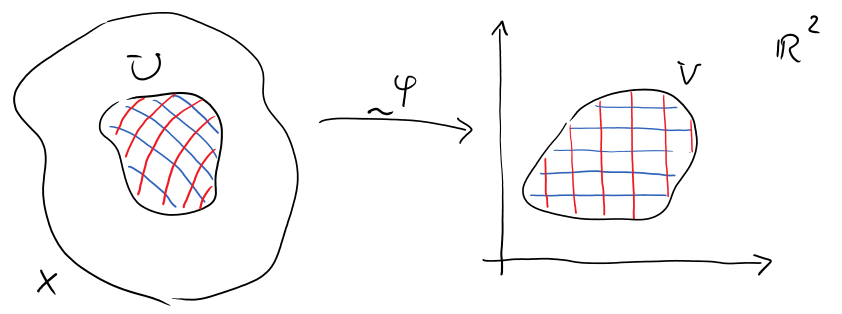
\includegraphics[width=.65\textwidth]{figures/chart.png}};
	\end{tikzpicture}
\end{figure}

Indeed, more often we'll not address directly the map $\phi$ but its components $\phi = (x^1, \ldots, x^n)$. We'll usually say something like: let $(x^1, \ldots, x^n)$ be coordinates around\footnote{Usually this will imply, additionally, that $\phi(p) = 0$, so that we are taken $\im \phi$ to be a neighbourhood of the origin.} $p \in M$. This means we do not give much importance to $U$ either, as long as we know it contains our point of interest.

Finally, notice that when two charts $(U_1, \phi_1)$ and $(U_2, \phi_2)$ overlap, then they are automatically ``compatible'' on their intersection, since $\phi_2 \circ \phi_1^{-1} : \phi_1(U_1 \cap U_2) \isoto \phi_2(U_1 \cap U_2)$ defines an homeomorphism on them. These maps are called \textbf{transition maps} and sew together the different local descriptions of the space $M$.

\begin{definition}
	A \textbf{smooth manifold} is a topological space $M$ together with a \textbf{smooth atlas}, i.e. a collection $\mathcal A = \{(U_i, \phi_i)\}_{i \in I}$ of charts such that all the transition maps are $\Cinfty$-diffeomorphisms\footnote{Hence homeomorphisms which are differentiable infinitely many times.}.
\end{definition}

\begin{remark}
	We stress the last word of the definition: as any two overlapping charts are ``topologically comaptible'', the smoothness of the manifold is ensued by the differentiability of the transition maps.
\end{remark}

We conclude this brief introduction by noting that we rarely give an explicti atlas along with our manifolds. The reason is twofold:
\begin{enumerate}
	\item for most spaces (e.g. spheres, tori, projective spaces), geometers worked out their construction in terms of an atlas once, and then it is understood we are using that;
	\item we always assume the atlas to be \textbf{maximal}, that is, to contain every possible compatible chart (with a given starting set): as such a collection is clearly very large, it is impossible to give one explicitly.
\end{enumerate}

\section{Vector bundles}
On a smooth manifold we are interested in studying so-called differential objects: vectors and forms, as well as smooth functions supported on the manifold.

\begin{definition}
	A \textbf{map of smooth manifolds} $F:M \to N$ is a map from the manifold $M$ to the manifold $N$ which is locally represented by a differentiable function, i.e. for every $p \in M$, there exist a chart $(U, \phi)$ around $p$ and a chart $(V, \psi)$ around $F(p)$ such that $\psi \circ F \circ \phi^{-1}$ is a differentiable function in the usual sense.
\end{definition}

The space of differentiable maps from $M$ to $\R$ is denoted by $\Cinfty(M)$. It clearly is an $\R$-algebra, i.e. a ring whose addition makes it into an $\R$-module.

\begin{definition}
	A \textbf{vector bundle} on a smooth manifold $M$ is a map $\pi : E \to M$ from a smooth manifold $E$ called the \textbf{total space} to the manifold $M$ called the \textbf{base space} such that
	\begin{enumerate}
		\item $\pi^{-1}(p)$ is a vector space for any $p$,
		\item for each $p$, there is an open neighbourhood $U$ of $p$ and a diffeomorphism $\chi :\pi^{-1}(U) \isoto U \times \pi^{-1}(p)$ which is fiberwise an isomorphism of vector spaces and makes the following commute:
		\begin{diagram}
			\pi^{-1}(U) \arrow{d}{\pi} \arrow{r}{\chi} \& U \times \pi^{-1}(p) \arrow{dl}{\pr_1}\\
			U
		\end{diagram}
	\end{enumerate}
\end{definition}

Intuitively, a vector bundle is a smooth assignment of vector spaces to each point of a manifold. A consequence of this is that every fiber $\pi^{-1}(p)$ has the same dimension $r$, called the \textbf{rank} of the bundle.

\begin{definition}
	A \textbf{section} of a vector bundle $\pi : E \to M$ is any map $s : M \supseteq U \to E$ which is a left inverse of $\pi$ on $U$, i.e. \begin{eqalign}
		\pi \circ s = \id_U.
	\end{eqalign}
	If $U=M$, the section is said to be \textbf{global}.
\end{definition}

A section of a vector bundle can be more easily depicted as a smooth assignment of vectors of $E$, where the vector at $p \in M$ is taken from the fiber there.

The most important vector bundle in differential geometry is the \textbf{tangent bundle} $TM$. Its construction is somewhat technical so we refer to \cite{abate2011geometria}, but intuitively it is the vector bundle whose fiber at $p \in M$ is the space of tangent vectors at $p$, suitably defined. Global sections of $TM$ are called \textbf{vector fields} and the totality of them is denoted by $\fields(M)$.

Along with $TM$, we get the \textbf{cotangent bundle} $T^*M$, whose fibers are dual to those of $TM$. Global sections of $T^*M$ are called \textbf{differential $1$-forms} and the totality of them is denoted by $\Omega^1(M)$.

Finally, through fiberwise tensoring we get a \textbf{tensor bundle} $T^p_q M$ for each $p, q \in \N$. Global sections of $T^h_k$ are called \textbf{$h$-covariant, $k$-contravariant tensors}, or simply \textbf{tensors of type $(h, k)$}. Clearly $T^1 M = TM$ and $T_1 M = T^* M$. When after tensoring, we look at the skew-symmetric part of the tensors, we get an algebra called the \textbf{external algebra} of $M$. The product is denoted by $\wedge$, and is defined as
\begin{eqalign}
	\xi_1 \wedge \ldots \wedge \xi_q = \sum_{\sigma \in S_q} (-1)^{\sign \sigma} \xi_{\sigma(1)} \tens \ldots \tens \xi_{\sigma(q)}, \quad \forall \xi_1, \ldots, \xi_q \in T^*M.
\end{eqalign}
Skew-symmetric $k$-contravariant tensors are more commonly referred to as \textbf{differential $k$-forms}, and their collection is denoted by $\Omega^q(M)$. Skew-symmetric $h$-covariant tensors are more commonly referred to as \textbf{$h$-vectors} (or, more generally, \textbf{multivectors}) and their collection is denoted by $\fields^q(M)$.

\subsection{Pullback and pushforward}
Any smooth map $F: M \to N$ induces morphisms between the respective tangent and cotangent bundles. In this section, let $p$ will designate a point of $M$ and $q$ a point of $N$.

\begin{construction}
\label{const:diff_at_P}
	For \textbf{vectors}, at each point $p$ of $M$ there's a well-defined map of fibers
	\begin{eqalign}
		(F_*)_p = dF_p : T_p M \to T_{F(p)}N
	\end{eqalign}
	called the \textbf{differential of $F$ at $p$}, whose intrinsic definition depends on the specific way the tangent bundle is defined. Anyway, once coordinates $(x^1, \ldots, x^m)$ are fixed around $p$ and coordinates $(y^1, \ldots, y^n)$ are fixed around $q$, its expression becomes\footnote{The subscript in $(F_*)_p$ is usually omitted when unnecessary, writing only $F_*$.}
	\begin{eqalign}
		F_* \left( X^h\vert_p \partial_h\vert_p \right) = X^h\vert_p\,\pder{F^k}{x^h}\vert_{F(p)}\, \partial_k\vert_{F(p)}
	\end{eqalign}
	where $\partial F^k /\partial x^h \vert_{F(p)}$ is the Jacobian of $F$ at $F(p)$ computed with respect to the chosen coordinates\footnote{This means that we should actually refer to the Jacobian of the local representation $\tilde F$ at the point $(x^1(p),\ldots,x^m(p))$.}.
\end{construction}

\begin{construction}
\label{const:dual_diff_at_P}
	The dual of $F_*$, in the sense of linear algebra, is a corresponding fiberwise morphism between the cotangent bundles, but in the opposite direction. Recall that $T^*_qN$ is the space of $\R$-valued functionals on $T_q N$. When $q = F(p)$, it's then natural to precompose any such functional with the differential of $F$ at $p$ to get a functional on $T_p M$. Diagrammatically, it is very intuitive:
	\begin{diagram}
		T_p M \arrow[dashed, swap]{dr}{F^* \xi} \arrow{r}{F_*} \& T_{F(p)}N \arrow{d}{\xi}\\[3ex]
		\& \R
	\end{diagram}
	Hence
	\begin{eqalign}
		F^* : T^*_{F(p)} N &\longto T^*_p M\\
		\xi &\longmapsto \xi \circ F_*
	\end{eqalign}
	Notice that $F^*\xi_q$ for $\xi_q \in T^*_qN$ is well defined provided that $F^{-1}(q)$ is defined uniquely, hence in the definition of $F^*$ we require that  \textbf{$F$ is a diffeomorphism}.  
	Then we can easily see that $F^*$ is the dual of $F_*$:
	\begin{eqalign}
	\end{eqalign} 
	where $X_p \in T_pM$ and $\xi_q \in T^*_qN$ with $q= F(p)$.
\end{construction}

We usually use vectors and covectors in the form of vector fields and differential forms. Thus we'd like to define a way to move sections along $F$.

\begin{construction}
\label{const:pushforward}
	For vector fields, this operation is called \textbf{pushforward}
	\begin{eqalign}
		F_* : \fields(M) &\longto \fields(N)\\
		X &\longmapsto F_*X
	\end{eqalign}
	such that
	\begin{eqalign}
		F_*X : N &\longto TN\\
		q &\longmapsto (F_*X)_q := dF_{F^{-1}(q)}(X_{F^{-1}(q)})
	\end{eqalign}
	Notice that this map is well defined if and only if $F$ is a diffeomorphism.
\end{construction}

\begin{construction}
\label{const:pullback}
	Conversely, the analogous map for differential forms, called the \textbf{pullback} is now well defined everytime:
	\begin{eqalign}
		F^* : \Omega^1(N) &\longto \Omega^1(M)\\
		\omega &\longmapsto F^*\omega
	\end{eqalign}
	such that
	\begin{eqalign}
		F^*\omega : M &\longto T^*M\\
		p &\longmapsto F^*_p\omega := \omega_{F(p)} \circ dF_p
	\end{eqalign}
\end{construction}

\begin{construction}
\label{const:pb_and_pf_of_tensors}
	We can extend both kinds of maps to \emph{homogeneous} tensors by having them act componentwise: for example, the last becomes
	\begin{eqalign}
		F^* : \Omega^k(N) &\longto \Omega^k(M)\\
		\omega_1 \wedge \ldots \wedge \omega_k &\longmapsto F^* \omega_1 \wedge \ldots \wedge F^*\omega_k.
	\end{eqalign}
	Notice the same restrictions as before apply. We stress it doesn't make sense to speak about pullback/pushforward of \emph{mixed} tensors since mixed tensors also have mixed variancy of the induced maps (you'd have to pullback one part of the tensor and pushforward another); unless $M=N$.
\end{construction}

\subsection{Distributions}
\begin{definition}
	A $k$-dimensional distribution $D$ on a smooth manifold $M$ is a subset of $TM$ such that $D_p = D \cap T_pM$ is a key dimensional subspace of $T_pM$ for each $p\in M$.
\end{definition}

The most common way to define a distribution on a manifold its through a set of generators.

\begin{definition}
	The distribution generated by the vector fields $X_1, \ldots, X_k \in \fields(M)$ is given pointwise by
	\begin{eqalign}
		D_p = \langle X_1\vert_p, \ldots, X_k\vert_p \rangle.
	\end{eqalign}
\end{definition}

\begin{definition}
	We say a $k$-dimensional distribution $D$ is \textbf{smooth} if, for any point $p \in M$, there exists an open neighbourhood $U$ of $p$ such that $D$ restricted to $U$ can be generated by $k$ vector fields of $\fields(M)$. Such a set of vector fields is called a \textbf{local frame} for $D$ on $U$.
\end{definition}

Evidently, a smooth distribution is again a vector bundle on $M$. Hence we can consider ``$D$-valued vector fields'', which are just section of $D$, i.e. vector fields with values in $D_p$ at each point $p \in M$. The totality of them is denoted by $\fields_D(M)$. 

\begin{definition}
	A distribution is called \textbf{involutive} if $\fields_D(M)$ is a Lie subalgebra of $\fields(M)$, i.e. if the Lie bracket of two sections of $D$ is again a section of $D$.
\end{definition}

The most useful kind of distributions are those giving or coming from \textbf{foliations}, i.e. partitions of $M$ into smooth submanifolds\footnote{In a \textbf{regular} folations, leaves have all the same dimension, otherwise the foliation is called \textbf{singular}.} called \textbf{leaves}. Then any foliation clearly induce a distribution given by the tangent spaces of the leaves. It's then natural to ask when the converse is true.

\begin{definition}
	An \textbf{integral submanifold} of a smooth distribution $D$ is a submanifold $S \subseteq M$ such that $TS = D$ on $S$.
\end{definition}

\begin{definition}
	A smooth distribution $D$ is said to be \textbf{integrable} if every point of $M$ is contained in an integral submanifold of $D$.
\end{definition}

\begin{definition}
	Let $D$ be a $k$-dimensional smooth distribution on an $n$-dimensional manifold $M$. A chart $(U,\phi)$ is \textbf{flat} for $D$ if
	\begin{enumerate}
		\item $\phi(U) = V \times W$ where $V$ is open in $\R^k$ and $W$ is open in $\R^{n-k}$,
		\item $(\partial_1, \ldots, \partial_k)$ is a local frame for $D$ on $U$.
	\end{enumerate}
	A distribution is called \textbf{completely integrable} if $M$ admits an atlas of flat charts for $D$.
\end{definition}

To say a chart on $U$ is flat for $D$ then means its integral submanifolds cut $U$ in directions parallel to the coordinates on $U$, i.e. every set of the form $\{x \in U \suchthat x^{k+1} = c^1, \ldots, x^n=c^{n-k}\}$ for a point $(c_1, \ldots, c_{n-k}) \in V$ (defined as above) is an integral submanifold of $D$ on $U$. The first bullet point in the definition says that the coordinates on $U$ can be naturally partitioned in ``parallel'' directions (contained and generating the integral submanifolds) and ``transverse'' directions (``orthogonal'' to the integral submanifolds).

The concepts of involutive, integrable and completely integrable smooth distribution are related by the following theorems:

\begin{proposition}
\label{prop:comp_int_is_int}
	Any smooth, completely integrable distribution is integrable.
\end{proposition}

\begin{proposition}
\label{prop:int_is_inv}
	Any smooth integrable distribution is involutive.
\end{proposition}

\begin{theorem}[{Frobenius, \cite[Teorema 3.7.11]{abate2011geometria}}]
\label{th:frobenius}
	Any smooth involutive distribution is completely integrable.
\end{theorem}

While the first two are relatively straightforward to prove, the third one is more involuted and technical.

\begin{diagram}
	\text{completely integrable} \arrow[Rightarrow]{r}{Prop.~\ref{prop:int_is_inv}} \& \text{integrable} \arrow[Rightarrow]{r}{Prop.~\ref{prop:comp_int_is_int}} \& \text{involutive} \arrow[Rightarrow, bend left]{ll}{Th.~\ref{th:frobenius}}
\end{diagram}

In the end, integrable, completely integrable and involutive mean the same thing.

\section{Exterior derivative}
\begin{definition}
	The \textbf{exterior derivative} is the unique family of \emph{graded $\R$-antiderivations} $d : \Omega^{p}(M) \to \Omega^{p+1}$ extending the differential defined by Construction~\ref{const:global_diff_and_dual}, i.e. satisfying the following axioms:
	\begin{enumerate}
		\item It is $\R$-linear,
		\item For any smooth function $f \in \C^\infty(M) = \Omega^0(M)$, $d$ is the global differential of $f$,
		\item It is a boundary map:
		\begin{eqalign}
			d^2 = 0,
		\end{eqalign}
		\item It is a graded antiderivation:
		\begin{eqalign}
			d(\omega \wedge \eta) = d\omega \wedge \eta +(-1)^{|\omega|} \omega \wedge d\eta.
		\end{eqalign}
	\end{enumerate}
\end{definition}

Existence and uniqueness can be easily proved by building up from the first axiom using the other two. In particular, if $\omega = \omega_{i_1, \ldots, i_p} dx^{i_1} \wedge \ldots \wedge dx^{i_p}$, then
\begin{eqalign}
	d\omega = \pder{\omega_{i_1, \ldots, i_p}}{x^{i_0}} dx^{i_0} \wedge dx^{i_1} \wedge \ldots \wedge dx^{i_p}
\end{eqalign}
where indices ranges over the dimension of the ambient manifold, and summation is implied.

\begin{definition}
	A form $\omega$ is said to be \textbf{closed} if $d\omega = 0$. It's said to be \textbf{exact} if $\omega = d\alpha$ for some form $\alpha$.
\end{definition}

Clearly, since $d^2 = 0$, \textbf{any exact form is closed}. The converse is not always true and this is the starting point of de Rham cohomology theory, which we'll see soon.

\begin{lemma}
\label{lemma:der_of_ext_power}
	For any $p \in \N$ and $\alpha \in \Omega^p(M)$, for every $k$,
	\begin{eqalign}
		d(d\alpha)^{\wedge k} = d(\underbrace{d\alpha \wedge \ldots \wedge d\alpha}_{\text{$k$ times}}) = 0
	\end{eqalign}
	that is, exterior powers of exact forms are closed.
\end{lemma}
\begin{proof}
	We proceed by induction on $k$. Indeed, for $k=1$ the statement is true by definition of $d$. Assume it is true for $k-1$, then
	\begin{eqalign}
		d\left((d\alpha\right)^{\wedge k}) &= d \left(d\alpha \wedge (d\alpha)^{\wedge k-1}\right)\\
		&= \cancel{d^2 \alpha} \wedge (d\alpha)^{k-1} + (-1)^{|d\alpha|} d\alpha \wedge \cancel{d\left(d\alpha^{\wedge k-1}\right)} = 0
	\end{eqalign}
\end{proof}
\begin{corollary}
\label{cor:ext_power_is_exact}
	Exterior powers of exact forms are again exact.
\end{corollary}
\begin{proof}
	\begin{eqalign}
		(d\alpha)^{\wedge k} = d\alpha \wedge (d\alpha)^{\wedge k-1}  + (-1)^{|\alpha|} \alpha \wedge d(\underbrace{(d\alpha)^{\wedge k-1}}_{=0}) = d\left(\alpha \wedge (d\alpha)^{\wedge k-1}\right).
	\end{eqalign}
\end{proof}

So as we noted above, any exact form is closed, meaning the $d$s form the coboundary maps for a cochain complex of differential forms:
\begin{diagram}
	\ldots \arrow{r}{d} \& \Omega^p(M) \arrow{r}{d} \& \Omega^{p+1}(M) \arrow{r}{d} \& \ldots
\end{diagram}
This is called the \textbf{de Rham complex} of $M$, and we can naturally associate a cohomology theory to it by taking homologies: let $\ker d_p = Z^p(M)$ be the susbpace of closed $p$-forms ($p$-\textbf{cocycles}) and $\im d_{p-1} = B^p(M)$ the subspace of exact $p$-forms ($p$-\textbf{coboundaries}). Then the \textbf{$p$-th de Rham cohomology} is defined as
\begin{eqalign}
	H^p_{dR}(M) = Z^p(M) / B^p(M).
\end{eqalign}
So de Rham cohomology encodes the failure of closed $p$ forms to be exact. Surprisingly, although its definition is intrinsecally dependent on the smooth structure of $M$, \textbf{de Rham cohomology is a topological invariant}, meaning
\begin{eqalign}
	M \underset{\cat{Top}}\iso N \implies H^\bullet_{dR}(M) \underset{\cat{Vec}} H^\bullet_{dR}(N)
\end{eqalign}

This is proven by proving the equivalence of the cohomology to the (purely topological) singular homology.

\subsection{Singular Homology}
We will now describe an homology theory which is entirely topological. Indeed, in this construction there's no need to assume $M$ to be a smooth manifold, any topological space will suffice.

\begin{definition}
	A \textbf{singular $r$-simplex} is any set of the form
	\begin{eqalign}
		\Delta^r = [P_0, \ldots, P_r]
	\end{eqalign}
	where $P_0, \ldots, P_r \in \R^r$ are affinely independent points and $[-]$ denotes the convex closure of its argument.
\end{definition}

Basically simplices are a lower and higher dimensional generalization of triangles: $\Delta^0$ is a point, $\Delta^1$ a segment, $\Delta^2$ a triangle, $\Delta^3$ a tetrahedron, and so on:

\begin{figure}[H]
	\centering
	\begin{tikzpicture}
		\node (image) at (0,0) {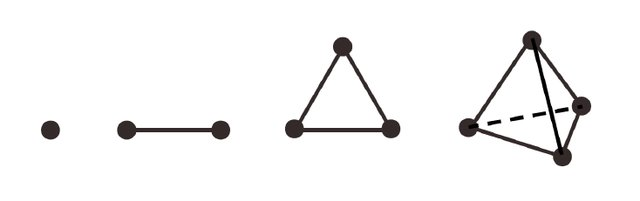
\includegraphics[width=.65\textwidth]{figures/simplices.jpg}};
	\end{tikzpicture}
\end{figure}

\begin{definition}
	A \textbf{singular $r$-simplex in a topological space $M$} is a continuous map $\sigma^r : U \to M$ where $U$ is an open neighbourhood of a $\Delta^r \subseteq \R^r$.
\end{definition}

By abuse of terminology, often we'll call $r$-simplex in $M$ the image of $\sigma^r$.

\begin{construction}
	Using the family of singular $r$-simplices in a topological space $M$ as generators, we can build a free $R$-module $C_r(M; R)$ for all commutative rings $R$ (usually $R$ is $\Z$, $\Q$, $\R$ or $\C$.). An element of such module is called an \textbf{$r$-chain} and it is a formal sum of $r$-simplices in $M$ with coefficients taken from $R$.
\end{construction}

\begin{definition}
	The \textbf{boundary} of an $r$-simplex $\sigma^r$ of $M$ is the $(r-1)$-chain $\partial \sigma^r$ defined as
	\begin{eqalign}
		\partial \sigma^r := \sum_{k=0}^r (-1)^k [P_0, \ldots, \hat{P_k}, \ldots, P_r]
	\end{eqalign}
	where $\hat{-}$ means we are skipping the term underneath.
\end{definition}

The terms, without sign, appearing in the summation defining $\partial \sigma^r$ are called \textbf{faces} of the simplex. Thus the boundary of a simplex is the alternating sum of its faces.

By $R$-linear extension, the boundary construction induces a (family of) map(s) $\partial : C_r(M; R) \to C_{r-1}(M; R)$, called the \textbf{boundary map(s)}.

\begin{lemma}
	The boundary maps are boundary maps in the sense of homological algebra, i.e.
	\begin{eqalign}
		\partial_{r-1} \partial_r = 0
	\end{eqalign}
\end{lemma}
\begin{proof}
	For conciseness sake, define
	\begin{eqalign}
		[\hat{h}, \hat{k}] = [p_0, \ldots, \hat{p_h}, \ldots, \hat{p_k}, \ldots, p_r].
	\end{eqalign}
	Notice to show the claim it suffices to prove it for a single, arbitrary $r$-simplex, as they generate $C_r(M; R)$. Then it is just a matter of computation. We just need to be careful substituting the second $\partial$ as indices for it have to be properly shifted:
	\begin{eqalign}
		\partial (\partial [p_0, \ldots, p_r]) &= \sum_{k=0}^r (-1)^k \partial [\hat{k}]\\
		&=\sum_{k=0}^r (-1)^k \left( \sum_{h=0}^{k-1} (-1)^h [\hat{h}, \hat{k}] + \sum_{h=k+1}^r (-1)^{h-1} [\hat{k}, \hat{h}] \right)\\
		&= \sum_{0 \leq h < k \leq r} (-1)^{k+h} [\hat{h}, \hat{k}] - \sum_{0 \leq k < h \leq r} (-1)^{k+h} [\hat{h}, \hat{k}] = 0,
	\end{eqalign}
	The very last equality is proven by swapping the indices of one summation (both will do) -- as its apparent this operation doesn't add nor remove any term; and simply noticing we then get two equal things subtracted, hence zero.
\end{proof}

Chains $\sigma^r \in C_r$ such that $\partial \sigma^r = 0$ are called \textbf{cycles} ($\sigma^r \in Z^r(M; R) = \ker \partial_r$ in symbols), while when $\partial \delta = \sigma$ for some $\delta \in C_{r+1}$ we speak of \textbf{boundaries} (in symbols $\sigma^r \in B^r(M; R) = \im \partial_{r+1}$).

\begin{definition}
	The \textbf{$r$-th singular homology of $M$ with coefficients in $R$} is
	\begin{eqalign}
		H_r(M; R) := \ker \partial_r / \im \partial_{r+1} = Z^r(M; R) / B^r(M; R)
	\end{eqalign}
\end{definition}

\subsection{de Rham's Theorem}
\label{subsec:de_rham}
Unlike de Rham cohomology, singular homology is a topological construction. On the other hand, on a smooth manifold $M$ we could have defined a ``smooth version'' by asking the maps $\sigma^r : U \to M$ to be not just continuous but smooth. Eventually, the two constructions turn out to be equivalent so we don't distinguish them in the following notation, but it's important to point out this is where the bridge between topological and \emph{differential} structure is crossed.

The aim of this section is then to prove smooth singular homology can be computed as well using de Rham cohomology, thus an easier and more tame machinery. To link the two, we'll use the natural pairing of differential forms and smooth simplicial chains given by integration:
\begin{eqalign}
	(-,-) : C^r(M; \R) \times \Omega^r(M) &\longto \R\\
	(\sum_{i=1}^n \alpha_n \sigma^r_n, \omega) &\longmapsto \int_C \omega := \sum_{i=1}^n \alpha_n \int_{\sigma^r_n} \omega
\end{eqalign}
Notice we fixed $R=\R$ for the coefficients of the homology as to get reals out of the integral.

A classical result links homological properties of differential forms to those of smooth simplicial chains:

\begin{theorem}[Stokes]
\label{th:stokes}
	Let $\omega \in \Omega^r(M)$ and $C$ be a smooth $(r+1)$-chain. Then
	\begin{eqalign}
		\int_{\partial C} \omega = \int_C d\omega
	\end{eqalign}
\end{theorem}

\begin{lemma}
	The integral pairing passes to homology and cohomology, i.e. the pairing
	\begin{eqalign}
		[-, -] : H_r(M; \R) \times H^r_{dR}(M) \longto \R
	\end{eqalign}
	defined by
	\begin{eqalign}
		[\overline C, \overline \omega] = (C, \omega)
	\end{eqalign}
	is a well-defined bilinear form.
\end{lemma}
\begin{proof}
	Choose $C' \in C^{r+1}(M; \R)$ and $\omega' \in \Omega^{r-1}$, then
	\begin{eqalign}
		C + \partial C' \in \overline C, \quad \omega + d\omega' \in \overline \omega
	\end{eqalign}
	so that to show well-definedness we simply need to show the result does not depend on $C'$ and $\omega'$. Indeed, applying the extended definition of the integral, Stokes' Theorem and recalling $\partial C=0$ and $d\omega = 0$ by definition of (co)homology, we get:
	\begin{eqalign}
		[\overline C, \overline\omega] &= (C + \partial C', \omega + d\omega')\\
			&= \int_C \omega + \int_{\partial C'} \omega + \int_C d\omega' + \int_{\partial C'} d\omega'\\
			&= \int_C \omega + \int_{C'} d\omega + \int_{\partial C} \omega' + \int_{\partial^2 C'} \omega' = (C, \omega).
	\end{eqalign}
	Bilinearity is then evident.
\end{proof}

\begin{theorem}[de Rham]
\label{th:de_rham}
	The bilinear form $[-,-]$ defined above is non-degenerate, hence it induces an isomorphism
	\begin{eqalign}
		H_r(M; \R) \isoin{\Vec} H_{dR}^r(M)
	\end{eqalign}
\end{theorem}

\begin{theorem}[Poincarè's duality]
	Let $M$ be a \emph{compact} orientable manifold of dimension $m$. The map
	\begin{eqalign}
		\langle -, - \rangle : H_{dR}^r(M) \times H_{dR}^{m-r}(M) &\longto \R\\
		( \overline \omega, \overline \eta) &\longmapsto \int_M \omega \wedge \eta
	\end{eqalign}
	is a well-defined, non-degenerate bilinear form, implying $H_{dR}^r(M) \isoin\Vec H_{dR}^{m-r}(M)$.
\end{theorem}
\begin{proof}[Proof sketch]
	For a compact orientable manifold we can produce a triangulation of $M$, that is, an $m$-chain homeomorphic to $M$ itself. By compactness of $M$, the chain must be a cycle since $\partial M = 0$. However it can't be the boundary of anyhting bigger since it is of maximal dimension. Then by de Rham's again,
	\begin{eqalign}
		\int_{\Delta_m} \omega \wedge \eta \neq 0
	\end{eqalign}
	proving the theorem.
\end{proof}

\begin{definition}
	The \textbf{Euler characteristic} of $M$ is the alternating sum of the dimensions of the homology groups of $M$:
	\begin{eqalign}
		\chi_M = \sum_{n=0}^{\dim M} (-1)^n \dim H_n(M)
	\end{eqalign}
\end{definition}

\begin{corollary}
	Any odd-dimensional compact orientable smooth manifold has $\chi_M = 0$.
\end{corollary}
\begin{proof}
	By de Rham's Theorem and Poincarè's duality.
\end{proof}

\paragraph{Induced maps.} \label{par:ind_maps_on_de_rham} Singular homology and de Rham cohomology are actually a family of functors, in the sense that maps between manifolds induce also maps between their cohomology groups in a way that is well-behaved with respect to composition. Indeed, if $f:X \to Y$ is a smooth map, it also brings singular simplices on $X$ to singular simplices on $Y$:
\begin{diagram}
	\& \Delta^n \arrow{dl}{\sigma} \arrow[dashed]{dr}{f \circ \sigma}\\
	X \arrow{rr}{f} \& \& Y
\end{diagram}
thereby producing a morphism $f^* : H_n(X; R) \to H_n(Y; R)$. The same thing happens for cohomology groups, although with a different variancy, by using the pullback of forms (Construction~\ref{const:pullback}), so we get a morphism $f^\sharp : H_{dR}^n(Y) \to H_{dR}^n(X)$.

When $f_0, f_1 : M_1 \to M_2$ are smooth maps, to say they're \textbf{smoothly homotopic} means there is a ``smooth map interpolating between the two'', i.e. a smooth map
\begin{eqalign}
	h: M_1 \times [0,1] \to M_2,\ (p,t) \mapsto h_t(p)
\end{eqalign}
such that
\begin{eqalign}
	h_0 = f_0, \quad h_1 = f_1.
\end{eqalign}
Then it can be shown that \textbf{the whenever $f_0$ and $f_1$ are homotopic, they induce the same homeomorphisms $f_0^\sharp$ and $f_1^\sharp$ on the de Rham cohomology groups}.

\section{Interior product}
\begin{definition}[Interior product]
	Let $X \in \fields(M)$. The \textbf{interior product} with $X$ of a $(p+1)$-differential form $\omega$ is the unique $p$-differential form defined by
	\begin{eqalign}
		\ipr{X} \omega (X_1, \ldots, X_p) = \omega(X, X_1, \ldots, X_p), \quad \forall X_1, \ldots, X_p \in \fields(M).
	\end{eqalign}
\end{definition}

\begin{property}
	Let $X \in \fields(M)$, $\omega \in \Omega^p(M)$ and $\eta \in \Omega^q(M)$. Then the following hold:
	\begin{enumerate}
		\item $\ipr{X}$ is a boundary map:
		\begin{eqalign}
			\ipr{X}^2 = 0.
		\end{eqalign}
		\item $\ipr{X}$ is an \textbf{graded antiderivation}:
		\begin{eqalign}
		\label{eq:int_prod_graded_antid}
			\ipr{X}(\omega \wedge \eta) = (\ipr{X} \omega) \wedge \eta + (-1)^p \omega \wedge (\ipr{X} \eta).
		\end{eqalign}
		\item $\ipr{X}$ commutes with the Lie derivative along $X$:
		\begin{eqalign}
			\Lie{X} \ipr{X} = \ipr{X} \Lie{X}.
		\end{eqalign}
		\item Cartan's magic formula:
		\begin{eqalign}
		\label{eq:cartan_magic_formula}
			\Lie{X} \omega = d(\ipr{X} \omega) + \ipr{X} (d \omega).
		\end{eqalign}
	\end{enumerate}
\end{property}

\subsection{Integration}
\begin{definition}
	A \textbf{volume form} on the $n$-dimensional manifold $M$ is given by an $n$-differential form
\end{definition}

\end{document}
	\documentclass[main.tex]{subfiles}
\begin{document}

\chapter{Symplectic geometry}
\section{Symplectic vector spaces}
\begin{definition}
	A \textbf{symplectic form} is a non-degenerate, skew-symmetric bilinear form. A vector space $V$ equipped with a symplectic form on $V$ is called a \textbf{symplectic vector field}.
\end{definition}

Notice the analogy to an inner-product space, where skew-symmetry of the form is replaced by simple symmetry. Indeed, some results generalize as they depend only on the non-degeneracy of the bilinear form, for instance partial application of the form $\Omega$ fixes a canonical isomorphism of $V$ and its dual:
\begin{eqalign}
\label{eq:iso_induc_sym_form}
	\tilde\Omega : V &\longto V^*\\
	v &\longmapsto \Omega(v, -);
\end{eqalign}
On the other hand, the theory of inner product spaces and that of symplectic spaces start to diverge very early on:

\begin{theorem}
\label{th:decomp_th}
	Let $V$ be a finite-dimensional $\R$-vector space. Let $\Omega$ be a skew-symmetric, bilinear map on $V$. Then there exists a basis
	\begin{eqalign}
		B= \{ u_1, \ldots, u_k, e_1, \ldots, e_n, f_1, \ldots, f_n \}
	\end{eqalign}
	of $V$ such that
	\begin{enumerate}
		\item $\Omega(u_i, v) = 0$ for any $v \in V$ and $i \leq k$,
		\item $\Omega(e_i, e_j) = \Omega(f_i, f_j) = 0$ for any $i, j \leq n$,
		\item $\Omega(e_i, f_j) = \delta^i_j$ for any $i, j \leq n$,
	\end{enumerate}
\end{theorem}
\begin{proof}
	Let
	\begin{eqalign}
		U = \{ u \in V \suchthat \Omega(u,v) = 0\ \forall v \in V\}.
	\end{eqalign}
	This is a non-empty set since $0 \in U$ and it is the kernel of $\tilde\Omega$ defined in eq.~\eqref{eq:iso_induc_sym_form}, hence it is a linear subspace of $V$. Therefore if we let $u_1, \ldots, u_k$ be a basis for $U$ (letting $k = \dim U$), the first item is proved.

	We'll now build by induction a decomposition
	\begin{eqalign}
	\label{eq:symp_decomp}
		V = U \dir \langle e_1, f_1 \rangle \dir \ldots \langle e_n, f_n \rangle.
	\end{eqalign}
	Let $W$ be a complement of $U$ (i.e. a subspace of $V$ such that $U \dir W = V$). Unless $k=\dim V$ (in which case the theorem is vacuously proved), $W \neq 0$. Then we can select a non-zero vector $e_1$ from $W$, for which there has to be at least another $f_1 \in W$ such that $\Omega(e_1, f_1) \neq 0$. Otherwise $\Omega(e_1, w) = 0$ for every $w \in W$ implying $\Omega(e_1, v) = 0$ for any $v \in V$, since when $v \in U$ we already know $\Omega(e_1, v) = -\Omega(v, e_1) = 0$ by definition of $U$. But $U \cap V = 0$ and $e_1 \neq 0$ exclude this possibility.

	Thus we choose $e_1, f_1 \in W$ such that, up to rescaling, $\Omega(e_1, f_1) = 1$. Notice, moreover, that the two vectors are linearly independent, else $\Omega$ would be zero on them by skew-symmetry. Thus we can add $e_1$ and $f_1$ to our basis, let $W_1 = \langle e_1, f_1 \rangle$, and if $W_1 = W$ we are done. Conversely, define
	\begin{eqalign}
		W_1^\Omega = \{w \in W \suchthat \Omega(w, w_1) = 0\ \forall w_1 \in W_1\}
	\end{eqalign}
	which is a sort of ``$\Omega$-orthogonal space'' of $W_1$ inside $W$. As before, we can select a non-zero $e_2$ from $W_1^\Omega$ for which there must exist a $f_2 \in W_1^\Omega$ such that $\Omega(e_2, f_2) = 1$ up to rescaling, or $e_2$ would fall in $U$ since $U \dir W_1 \dir W_1^\Omega = V$. We understand then our process can go on as long as $W_n \neq W$, giving us a basis which satisfies (2) because each $e_i$ (resp. $f_i$) lives in the ``$\Omega$-orthogonal space'' of the other $e_i$ (resp. $f_i$), and (3) for the same reason plus the fact we make a suitable rescaling at each step.
\end{proof}
\begin{corollary}
\label{cor:can_form}
	The form $\Omega$, with respect to the basis $B$, is represented as the following block matrix
	\begin{eqalign}
		\begin{pmatrix}
			0 & 0 & 0\\
			0 & 0 & I_n\\
			0 & -I_n & 0
		\end{pmatrix}.
	\end{eqalign}
\end{corollary}

\begin{remark}
	While the decomposition of $V$ we found in the previous proof is highly non-canonical (we made a lot of arbitrary choices!), the dimensions of the decomposition depend solely on $\Omega$. In particular, notice that $\Omega$ is non-degenerate iff $k=0$, hence we see immediately that, in light of Theorem~\ref{th:decomp_th}, \textbf{a symplectic vector space is always even-dimensional}.
\end{remark}

Corollary~\ref{cor:can_form} prescribes we can always find a ``nice'' basis for $V$ in which $\Omega$ can be represented by a \textbf{symplectic matrix}:
\begin{eqalign}
	\begin{pmatrix}
		0 & I_n\\
		-I_n & 0
	\end{pmatrix}
\end{eqalign}
Even if, as noted before, the choice of such a basis is far from unique, we'll refer to it as a \emph{canonical} basis.

\begin{definition}
	A subspace $W$ of a symplectic vector space $(V, \Omega)$ is said to be \textbf{symplectic} as well if $(W, \Omega\vert_W)$ is a symplectic vector space. If instead $\Omega\vert_W = 0$, the subspace is called \textbf{isotropic} and its $\Omega$-orthogonal is then called \textbf{coisotropic}. When a subspace is both isotropic and coisotropic, it's named \textbf{Lagrangian}. In particular, in the finite-dimensional case a Lagrangian subspace of a vector space $V$ is an isotropic subspace whose dimension is half that of $V$.
\end{definition}

Theorem~\ref{th:decomp_th} says that any finite dimensional $\R$-vector space endowed with a skew-symmetric bilinear map $\Omega$ can be decomposed into an isotropic subspace and a symplectic subspace. In particular the decomposition~\eqref{eq:symp_decomp} is a decomposition of $V$ into an isotropic subspace $U$ and $n$ minimal symplectic subspaces of the form $\langle e_i, f_i \rangle$. 

\begin{definition}
	A \textbf{symplectomorphism} is a linear map $\phi : (V, \Omega) \to (V', \Omega')$ between symplectic vector spaces $(V, \Omega)$ and $(V', \Omega')$ such that
	\begin{eqalign}
		\Omega'(\phi(u), \phi(v)) = \Omega(u,v), \quad \forall u,v \in V,
	\end{eqalign}
	or, alternatively, if $\phi^* \Omega' = \Omega$. Two symplectic vector spaces with a symplectomorphism between them are said \textbf{symplectomorphic} and denoted by $(V, \Omega) \underset{\cat{Symp}}\iso (V', \Omega')$.
\end{definition}

Hence, in the case of symplectic vector spaces, Theorem~\ref{th:decomp_th} says that
\begin{eqalign}
	(V, \Omega) \underset{\cat{Symp}}\iso (\R^{2n},\Omega_0)
\end{eqalign}
where $\Omega_0$ is the symplectic matrix when seen from the canonical basis of $\R^{2n}$.

\section{Symplectic manifolds}
Endowing the tangent bundle of a manifold with a symplectic structure, we get the differential analogue of a symplectic vector space:

\begin{definition}
	A \textbf{symplectic form} $\omega$ on a smooth manifold $M$ is a non-degenerate\footnotemark, closed, differentiable $2$-form on $M$. A \textbf{symplectic manifold} is a manifold $M$ equipped with a symplectic form on $M$.
	\footnotetext{In this context, non-degenerate means pointwise non-degenerate.}
\end{definition}

Therefore at each point $p \in M$ the tangent space $T_pM$ is a symplectic vector space with symplectic form $\omega_p$.

\begin{example}
\label{ex:eu_sp_sphere}
	\leavevmode
	\begin{enumerate}
		\item Any Euclidean space $\R^{2n}$ can be equipped with the following form
		\begin{eqalign}
			\omega_0 = \sum_{i=1}^n dx^i \wedge dy^i
		\end{eqalign}
		where we call $y^i$ the coordinate $x^{n+i}$. With this definition $\omega_0$ is, pointwise, the form $\Omega_0$ discussed previously. Moreover, it is closed as
		\begin{eqalign}
			d\omega_0 &= \sum_{i=1}^n d(dx^i \wedge dy^i)\\
			&= \sum_{i=1}^n d^2x^i \wedge y^i - dx^i \wedge d^2y^i = 0
		\end{eqalign}
		\item The $2$-sphere is a symplectic manifold. Indeed, consider its immersion in $\R^3$ defined as $S^2 = \{ x \in \R^3 \suchthat \|x\| = 1\}$. Then
		\begin{eqalign}
			T_xS^2 = \{ v \in \R^3 \suchthat \langle v, x \rangle = 0 \}
		\end{eqalign}
		can be made into a symplectic vector space by means of
		\begin{eqalign}
			\omega_x (u,v) := \langle x, u \times v \rangle, \quad \forall u,v \in T_xS^2.
		\end{eqalign}
		which trivially defines a differential form $\omega \in \Omega^2(S^2)$. Finally, since $\dim S^2 = 2$ and $d\omega$ is a 3-form, the form $\omega$ is necessarily closed.
	\end{enumerate}
\end{example}

Since $\dim T_pM = \dim M$, $M$ inherits the condition on the dimension of $T_pM$: $M$ must be even-dimensional. However this time, even-dimensionality is not a sufficient condition for a manifold to be symplectic. A further necessary condition is given by the following theorem.

\begin{theorem}
\label{th:symp_vol_form}
	Let $(M, \omega)$ be a symplectic manifold, with $\dim M = 2n$. Then the $n$-th exterior power of $\omega$ is a volume form, i.e. $(\omega^{\wedge n})_p \neq 0$ for any $p \in M$.
\end{theorem}
\begin{proof}
	The rank of $\omega^{\wedge n}$ is $2n$, so the claim makes sense. Choose $p \in M$ now, and fix a local frame $E_1, \ldots, E_n, F_1, \ldots, F_n$ around $p$ in such a way that  it is in $p$ a canonical basis as per Theorem~\ref{th:decomp_th}. Then:
	\begin{eqalign}
		\omega^{\wedge n}_p (E_1\vert_p, \ldots, E_n\vert_p, F_1\vert_p, \ldots, F_n\vert_p) &= \omega_p(E_1\vert_p, F_1\vert_p) \cdot \ldots \cdot \omega_p(E_n\vert_p, F_n\vert_p) = 1
	\end{eqalign}
	thus the form is everywhere positive.
\end{proof}
\begin{corollary}
	If $M$ is symplectic, it is orientable.
\end{corollary}

The obvious remark is then that non-orientable manifolds can't be symplectic even in the even-dimensional case; e.g. the projective plane does not admit a symplectic structure.

Other obstructions are given by topology. For example

\begin{theorem}
	The $2$-sphere is the only sphere admitting a symplectic structure.
\end{theorem}
\begin{proof}
	In Example~\ref{ex:eu_sp_sphere} we exhibited a symplectic structure for $S^2$, so only we need to prove any $S^{2n}$ with $n \geq 2$ does not admit one. Let $\omega \in \Omega^2(S^{2n})$ be a closed form. Recall $H^2_{dR}(S^{2n}) = 0$, as the only non-vanishing homologies (hence cohomologies by de Rham's Theorem) are the bottom and the top ones (i.e.  $H^i_{dR}(S^d) \neq 0$ iff $i \in \{0, d\}$, $H^0_{dR}(S^{d}) = H^{d}_{dR}(S^{d}) = \R$) and we assumed $n > 1$. By definition of cohomology, this means all closed $2$-forms are automatically exact, implying there exists an $\eta \in \Omega^1(S^{2n})$ such that $d\eta = \omega$. Hence, using Corollary~\ref{cor:ext_power_is_exact} and Stokes' Theorem:
	\begin{eqalign}
		\int_{S^{2n}} \omega^{\wedge n} = \int_{S^{2n}} (d\eta)^{\wedge n} = \int_{S^{2n}} d(\eta \wedge (d\eta)^{\wedge (n-1)}) = \int_{\partial S^{2n}} \eta \wedge (d\eta)^{\wedge (n-1)} = 0
	\end{eqalign}
	since $n$-spheres have no boundaries. Then, by Theorem~\ref{th:symp_vol_form}, it must be $\omega = 0$ thus not symplectic.
\end{proof}

\begin{remark}
	Notice \textbf{the proof can be generalized to any compact manifold with vanishing second cohomology}. Moreover, it shows a symplectic form cannot be exact on a compact manifold.
\end{remark}

\begin{definition}
	A submanifold $N$ of a symplectic manifold $(M, \omega)$ is a \textbf{symplectic submanifold} if $(N, \omega\vert_N)$ is symplectic.
\end{definition}
\begin{definition}
	A diffeomorphism $\phi : M \to N$, where $(M, \omega)$ and $(N, \eta)$ are symplectic manifolds, is called a \textbf{symplectomorphism} if
	\begin{eqalign}
		\phi^* \eta = \omega
	\end{eqalign}
\end{definition}

\begin{remark}
\label{rmk:inverse_ipr}
	As with symplectic vector spaces, a symplectic form induces a natural isomorphism of $\fields(M)$ with $\Omega^1(M)$, which is the extension of the pointwise isomorphism $\tilde\omega_p : T_pM \to T^*_pM$, defined as before by partial application:
	\begin{eqalign}
		\omega : \fields(M) &\longto \Omega^1(M)\\
				X &\longmapsto \ipr{X}\omega
	\end{eqalign}
	The inverse map is
	\begin{eqalign}
		\omega^{-1} : \Omega^1(M) &\longto \fields(M)
	\end{eqalign}
	and it is defined as to satisfy
	\begin{eqalign}
		\omega^{-1}(\ipr{X}\omega) = X.
	\end{eqalign}
\end{remark}

\subsection[The canonical symplectic structure on the cotangent bundle]{The canonical symplectic structure\\on the cotangent bundle}
The chief example of symplectic manifolds are cotangent bundles of smooth manifolds. In fact, there's a natural/canonical way to equip $M= T^*X$ with a symplectic structure. Notice that $\dim T^*X = 2\dim X$ so that, in principle, we can expect to assign a symplectic structure to arbitrary cotangent bundles. Clearly, as we've seen, dimensionality isn't the only obstruction so we need to exhibit a symplectic form.

The construction of the symplectic structure exploits a particular, naturally defined, $1$-form on $T^*X$. The symplectic form will then be it's exterior derivative.

\begin{construction}
	Let $\pi : T^*X \to X$ be the bundle projection. Notice that a differential $1$-form on $T^*X$ is a function $T^*X \to T^*T^*X$ (with the additional condition of being compatible with the fibers, more on this later) which is exactly the type of function $d\pi^*$ is. If we unpack its definition from Construction~\ref{const:global_diff_and_dual}, we get
	\begin{eqalign}
		\pi^* : T^*X &\longto T^*T^*X\\
		(x, \xi) &\longmapsto (\pi^{-1}(x),\, \xi \circ d\pi_{\pi^{-1}(x)})
	\end{eqalign}
	So the definition fails. We already knew this: we remarked that $F^*$ is well-defined if and only if $F$ is a diffeomorphism, which is certainly not the case for $\pi$. On the other hand, we can try to fix this pathology by finding another way to choose a ``canonical'' element from $\pi^{-1}(x)$ in the mapping expression of $\pi^*(x, \xi)$. Indeed, since $\pi$ is surjective, that's the only obstruction! And we clearly see that those $\pi^{-1}(x)$ can be unambiguously resolved by simply using the argument of the sought function. So we define the mapping
	\begin{eqalign}
		\alpha : T^*X &\longto T^*T^*X\\
		(x, \xi) &\longmapsto ((x, \xi), \xi \circ d\pi_{(x, \xi)})
	\end{eqalign}
	or, using the fiberwise duals (Construction~\ref{const:dual_diff_at_P}):
	\begin{eqalign}
		\alpha(x, \xi) = \pi^*_{(x, \xi)} \xi.
	\end{eqalign}
	This is clearly well-defined as the domain of $\pi^*_{(x,\xi)}$ is precisely $T^*_{(x,\xi)} T^*X$. The $1$-form we just defined is called \textbf{Liouville form} or \textbf{tautological one-form}.
\end{construction}

The name \emph{tautological} comes from the following property: for every $\mu \in \Omega^1(X)$,
\begin{eqalign}
	\mu^* \alpha = \mu
\end{eqalign}
where $\mu^*$ is the pullback of $\mu$ when seen as smooth map $X \to T^*X$.

Let's compute what this form looks like, fixing coordinates on the involved spaces. Notice, first, that coordinates on $X$ suffice to fix relevant coordinates on both $T^*X$ and $T^*T^*X$, by using the induced reference frames as bases for the fibers:

\begin{center}
	\begin{tabular}{c|l|l}
		\textbf{Space} & \textbf{Local frame} & \textbf{Coordinates}\\[1ex]
		\hline
		$X$ & \textcolor{gray}{(does not apply)} & $(x^1, \ldots, x^n)$\\[1ex]
		$T^*X$ & $(dx^1, \ldots, dx^n)$ & $(x^1, \ldots, x^n, \xi^1, \ldots, \xi^n)$\\[1ex]
		$T^*T^*X$ & $(dx^1, \ldots, dx^n, d\xi^1, \ldots, d\xi^n)$ & $(x^1, \ldots, x^n, \xi^1, \ldots, \xi^n, \chi^1, \ldots, \chi^{2n})$\\
	\end{tabular}
\end{center}

Basically, for $T^*X$ and $T^*T^*X$, the second half of the coordinates are just the components with respect to the local frame on their left\footnote{This is doable for any locally trivial vector bundle: any point $y \in E$ of a vector bundle $\pi: E \to M$ can be thought as a pair $(\pi(y), v)$ so that we use the coordinates of $M$ for the first component, and components with respect to the local frame induced by the coordinates of $M$ on $E_{\pi(y)}$ for the second.}.

When we focus on a single fiber \textbf{half of the coordinates become superfluous since are fixed by the choice of fiber}. Therefore a covector $\xi \in T^*_x X$ will be written as
\begin{eqalign}
	\xi = \xi_j(x) dx^j\vert_x,
\end{eqalign}
while $\chi \in T^*_{(x,\xi)} T^*X$ (a double covector?) as
\begin{eqalign}
	\chi = \chi_j(x,\xi) dx^j\vert_{(x,\xi)} + \chi_{j+n}(x,\xi) d\xi^j\vert_{(x,\xi)}.
\end{eqalign}

In this setting, $\pi : T^*X \to X$ is the following map
\begin{eqalign}
	\pi(x, \xi) = \pi(x^1, \ldots, x^n, \xi^1, \ldots, \xi^n) = (x^1, \ldots, x^n), \quad \forall (x,\xi) \in T^*X
\end{eqalign}
whose differential, expressed as its Jacobian matrix, is then
\begin{eqalign}
	d\pi_{(x, \xi)} = \begin{pmatrix}
		\partial_i \pi^j
	\end{pmatrix}\rvert_{(x, \xi)} = \begin{pmatrix}
		\bigpder{\pi^j}{x^i} & \bigpder{\pi^j}{\xi^i}
	\end{pmatrix}\rvert_{(x, \xi)} = \begin{pmatrix}
		I_n & 0
	\end{pmatrix}.
\end{eqalign}
Then
\begin{eqalign}
	\alpha(x, \xi) &= d\pi^*_{(x, \xi)}\xi = \xi \circ d\pi_{(x, \xi)} = \xi_j \cancelto{\delta^j_k}{\pder{\pi^j}{x^k}} dx^k\vert_{(x,\xi)} + \xi_j \cancelto{0}{\pder{\pi^j}{\xi^k}} d\xi^k\vert_{(x,\xi)} = \xi_k dx^k\vert_{(x,\xi)}
\end{eqalign}

The ``canonicity'' of $\alpha$ is also witnessed by the following fact:

\begin{theorem}
\label{th:canonicity_of_taut}
	Let $F : X_1 \isoto X_2$ be a diffeomorphism and $\alpha, \beta$ the Liouville forms respectively on $X_1$ and $X_2$. Call $\mathcal{F}=(F^{-1})^*$ the dual morphism induced by $F^{-1}$. Then $\mathcal F^* \beta = \alpha$.
	\begin{diagram}
	\label{diag:liouville}
		T^*X_1 \arrow{d}{\pi_1} \arrow{r}{\mathcal F} \& T^*X_2 \arrow{d}{\pi_2}\\
		X_1 \arrow{r}{F} \& X_2
	\end{diagram}
\end{theorem}
\begin{proof}
	For each $(x, \xi) \in T^*X_1$,
	\begin{eqalign}
		\mathcal{F}(x, \xi) = (F(x), (F^{-1})^*_{F(x)}\xi),
	\end{eqalign}
	so that
	\begin{eqalign}
		(\mathcal F^* \beta)_{(x, \xi)} &= \beta_{\mathcal F(x,\xi)} \circ d\mathcal F_{(x, \xi)}\\
		&= ((\pi_2)^*_{\mathcal F(x,\xi)} (F^{-1})^*_{F(x)}\xi) \circ d\mathcal F_{(x, \xi)}\\
		&= \xi \circ d(F^{-1})_{F(x)} \circ d(\pi_2)_{\mathcal F(x,\xi)} \circ d\mathcal F_{(x, \xi)}\\
		&= \xi \circ d(F^{-1} \circ \pi_2 \circ \mathcal F)_{(x, \xi)} \comment{by chain rule}\\
		&= \xi \circ d(\pi_1)_{(x,\xi)} \comment{by Diagram~\ref{diag:liouville}}\\
		&= (\pi_1)^*_{(x, \xi)} \xi = \alpha_{(x,\xi)};
	\end{eqalign}
	which amounts to the thesis.
\end{proof}

\begin{definition}
	The \textbf{canonical symplectic form} on $T^*X$ is
	\begin{eqalign}
		\omega = -d\alpha
	\end{eqalign}
\end{definition}

Notice the minus sign, that's unavoidable and rigs pretty much all symplectic geometry.

With the same coordinates we used before, $\omega$ is
\begin{eqalign}
	\omega &= -d\alpha\\
	&= - d(\xi_j dx^j)\\
	&= - \cancelto{0}{\frac{\partial \xi_j}{\partial x^i}} dx^i \wedge dx^j - \cancelto{\delta^i_j}{\frac{\partial \xi_j}{\partial \xi_i}} d\xi_i \wedge dx^j\\
	&= dx^i \wedge d\xi_i
\end{eqalign}

\section{Symplectomorphisms and Lagrangian submanifolds}
Theorem~\ref{th:canonicity_of_taut} says the pullback $(f^{-1})^* : T^*X_1 \to T^*X_2$ is a symplectomorphism. In particular, when $X=X_1=X_2$, there's a natural morphism of groups,
\begin{diagram}
	\Diff(X) \arrow[hookrightarrow]{r} \& \Symp(T^*X, \omega),
\end{diagram}
whose domain is the group of diffeomorphisms of $X$ and whose codomain is the group of symplectomorphisms of $(T^*X, \omega)$. Recall that $X$ lives inside $T^*X$ as its zero section, thus the morphism is actually an inclusion, justifying its depiction by an hooked arrow. However, this map is not onto, since not all symplectomorphism arise in this way: for instance, translation along fibers of $T^*X$ is not in the image.

This leaves us with the problem of finding these additional symplectomorphisms. If diffeomorphisms of the base space are too few to induce all of them, conversely diffeomorphisms of the total space are too many and we need to weed out all the ones which aren't preserving the symplectic structure.

Luckily, a new geometric concept comes to help:

\begin{definition}
	A submanifold $Y$ of a symplectic manifold $(M, \omega)$ is called \textbf{Lagrangian} when
	\begin{enumerate}
		\item $\dim Y = \frac12 \dim M$ and
		\item $Y$ is \textbf{isotropic}, i.e. if $\iota: Y \into M$ is the embedding of $Y$, then $\iota^* \omega = 0$
	\end{enumerate}
\end{definition}

These submanifolds are closely related to symplectomorphisms. A first hint comes from the following result.

\begin{exercise}
\label{ex:lagrangian_submanifolds_of_cotangent_bundles}
	Let $M = T^*X$ for a smooth manifold $X$, along with its canonical symplectic structure. Prove the graph of $\alpha \in \Omega^1(X)$ defines a Lagrangian submanifold of $M$ if and only if $\alpha$ is closed, that is $d\alpha =0$.
\end{exercise}
\begin{proof}
	Indeed, let $\Gamma$ be the graph of $\alpha$. Then $\Gamma$ is trivally an embedded submanifold of $M$ of dimension $\frac12 \dim M$. Fix now coordinates as in the construction of Liouville's form. If we consider the inclusion $\iota : X \simeq \Gamma_\alpha X \into M$ whose differential respect to $X$ and $M$ local coordinates is 
	\begin{eqalign}
		d\iota = \begin{pmatrix}
			\delta^i_j \\
			\partial_j \alpha^i
		\end{pmatrix}
	\end{eqalign}
	from which
	\begin{eqalign}
		\iota^* \omega &= (dx^i \wedge d\xi_i) \circ d\iota = dx^i \wedge (\partial_j \alpha_i) dx^j = - (\partial_j \alpha_i) dx^j \wedge dx^i = - d (\alpha_i dx^i) = - d\alpha
	\end{eqalign}
	then the claim follows immediately.
\end{proof}

Consider now two symplectic manifolds $(M_1,\omega_1)$ and $(M_2, \omega_2)$, with the same dimension $\dim M_1 = \dim M_2$. We can endow $M_1 \times M_2$ with two different symplectic structures
\begin{eqalign}
	\omega_\pm = \pr_1^*\omega_1 \pm \pr_2^*\omega_2
\end{eqalign}
where $\pr_.$ denote a projection map onto $M_.$.

\begin{theorem}
\label{th:char_of_symplectomorphism}
	A diffeomorphism $\phi : M_1 \to M_2$ is a symplectomorphism if and only if its graph submanifold
	\begin{diagram}
		\Gamma_\phi = \{(p, \phi(p)) \suchthat p \in M_1\} \arrow[hookrightarrow]{r}{\iota} \& M_1 \times M_2
	\end{diagram}
	is Lagrangian with respect to $\omega_-$.
\end{theorem}
\begin{proof}
	As $\dim M_1 = \dim M_2$ (because they're diffeomorphic through $\phi$),
	\begin{eqalign}
		\dim \Gamma_\phi = \dim M_1 = \frac12 \dim (M_1 \times M_2).
	\end{eqalign}
	Moreover, we have
	\begin{eqalign}
		\iota^*\omega_- = \iota^*\pr_1^* \omega_1 - \iota^*\pr_2^* \omega_2 = (\pr_1 \circ \iota)^* \omega_1 - (\pr_2 \circ \iota)^* \omega_2
	\end{eqalign}
	Since\footnote{With abuse of notation, we call $\iota$ both the inclusions $\Gamma_\phi \into M_1 \times M_2$ and $M_1 \into M_1 \times M_2$ where in the second case the isomorphism $M_1 \simeq \Gamma_\phi$ is used. } $\iota$ sends $p \mapsto (p,\phi(p))$, composing with the projection on the first component yields $\id_{M_1}$, and composing with the other projection yields $\phi$. Thus
	\begin{eqalign}
		\iota^*\omega_- = \id^*\omega_1 - \phi^*\omega_2
	\end{eqalign}
	Implying
	\begin{eqalign}
		\phi^*\omega_2 = \omega_1 \iff \iota^*\omega_- = 0
	\end{eqalign}
	which is the claim we wanted to prove.
\end{proof}

\begin{remark}
	The theorem \emph{does not} state any Lagrangian submanifold is the graph of a symplectomorphism: it is assumed, a fortiori, that $\phi$ is a diffeomorphism.
\end{remark}

\subsection{Symplectomorphisms $T^*X_1 \to T^*X_2$ and generating functions}
Theorem \ref{th:char_of_symplectomorphism}, combined with Exercise~\ref{ex:lagrangian_submanifolds_of_cotangent_bundles}, gives us a systematic way to produce symplectomorphisms of a cotangent space starting from an exact form $df$.

\begin{construction}
	In the case $M_1 = T^*X_1$ and $M_2 = T^*X_2$, along with their canonical symplectic structure, then
	\begin{eqalign}
		T^*X_1 \times T^*X_2 = T^*(X_1 \times X_2)
	\end{eqalign}
	and the space is symplectic with symplectic form
	\begin{eqalign}
		\omega_- = - d(\pr_1^*\alpha_1 - \pr_2^*\alpha_2).
	\end{eqalign}
	On the other hand, the canonical symplectic form on $T^*(X_1 \times X_2)$ is
	\begin{eqalign}
		\omega_+ = - d(\pr_1^*\alpha_1 + \pr_2^*\alpha_2)
	\end{eqalign}
	By Exercise~\ref{ex:lagrangian_submanifolds_of_cotangent_bundles}, we know how to construct Lagrangian manifolds on $T^*(X_1 \times X_2)$ with respect to its canonical symplectic structure as cotangent bundle. However, Theorem~\ref{th:char_of_symplectomorphism} refers to the other symplectic structure of $T^*(X_1 \times X_2)$, obtained from its product structure. Thus we leverage the following procedure:
	\begin{enumerate}
		\item Produce a Lagrangian submanifold of $T^*(X_1 \times X_2)$ with respect to $\omega_+$: choose any function $f \in \Cinfty(X_1 \times X_2)$ and consider $\Gamma_{df} = \{(x,y,d_x f, d_y f) \suchthat (x,y) \in X_1 \times X_2\}$.
		\item Twist the graph to $\tilde\Gamma_{df} = \{(x,y,d_xf,-d_yf) \suchthat (x,y) \in X_1 \times X_2\}$ (because the only difference between $\omega_+$ and $\omega_-$ is exactly this twist on the second factor) to get a Lagrangian submanifold with respect to $\omega_-$.
		\item For $\tilde\Gamma_{df}$ to be the graph of a diffeomorphism $\phi : T^*X_1 \isoto T^*X_2$, it needs to satisfy a local condition: it must not be ``vertical'' at any point on the $T^*X_1$-$T^*X_2$ plane, that is, the projection $\pr_1 : \tilde\Gamma_{df} \to T^*X_1$ must have no critical points. This means
		\begin{eqalign}
		\label{eq:canonical_transf_from_gen_funcs_invertibility}
			\det \left( \spder{f}{y^j}{x^i} \right) \neq 0
		\end{eqalign}
		If this is satisfied, then $\phi$ sends the first and third component of a point in $\tilde\Gamma_{df}$ to the second and fourth components:
		\begin{eqalign}
			\phi : (x,\xi) \mapsto (y,\eta)
		\end{eqalign}
		where
		\begin{eqalign}
		\label{eq:canonical_transf_from_gen_funcs}
			\begin{cases}
				\xi_i = \bigpder{f}{x^i}(x,y)\\
				\eta_i = -\bigpder{f}{y^i}(x,y)
			\end{cases}
		\end{eqalign}
		in such a way that $\tilde\Gamma_{df} = \{(x,y,\xi (x,y),\eta (x,y)) \suchthat (x,y) \in X_1 \times X_2\} = \Gamma_\phi$. Condition eq.~\eqref{eq:canonical_transf_from_gen_funcs_invertibility} ensures the invertibility of eq.~\eqref{eq:canonical_transf_from_gen_funcs} and then the well-definiteness of $\phi$. 
	\end{enumerate}
\end{construction}

Eventually, in the case $X_1 = X_2 = X$, we just explained geometrically how \textbf{canonical transformations} of a phase-space manifold arise from \textbf{generating functions} $f \in \Cinfty(X \times X)$.

\section{Darboux's Theorem}
We'll now pursue a local description of symplectic manifolds. For this section, refer to \cite[Section 1.4]{cannas2005symplectic} and \cite[Section 1.5]{cannas2005symplectic}.

\subsection{Tubular neighbourhoods}
\begin{definition}
	Given a closed embedding ${\iota : X \into M}$ of a $k$-dimensional submanifold $X$ into its $n$-dimensional ambient manifold $M$, its \textbf{normal bundle} is
	\begin{eqalign}
		NX := TM/TX
	\end{eqalign}
	defined pointwise on $X$.
\end{definition}

Any section $\sigma: X \to NX$ of $NX$ can be interpreted as a deformation of $X$. Then, the zero section $\sigma_0: x \mapsto 0$ is $X$ itself, i.e. $\iota_0 : X \into NX$ with $\iota_0 (X) = \sigma_0 (X)$.

\begin{definition}
	A \textbf{tubular neighbourhood} of $X$ is an open neighbourhood $U$ of $\iota(X)$ in $M$ diffeomorphic to a convex\footnotemark\ neighbourhood $U_0 \subseteq NX$ of the zero section of the normal bundle.
	\footnotetext{In a vector space, a subset is convex if any convex combination of elements of the subset is still in the subset. In a vector bundle a neighbourhood is convex if its intersection with each fiber is convex.}
\end{definition}

The convexity condition means that $U_0 \cap N_xX$ has to be convex as a subset of the vector space $N_x X$.

Hence the situation is the following:
\begin{diagram}
	NX \arrow[relation=\supseteq]{r} \&[-3ex] U_0 \arrow[shift left]{dr}{\pi_0} \arrow{rr}{\phi} \& \& \arrow[dashed, shift left]{dl}{\pi} U \arrow[relation=\subseteq]{r} \&[-3ex] M\\
	\& \& X \arrow[hookrightarrow, shift left]{ur}{\iota} \arrow[hookrightarrow, shift left]{ul}{\iota_0}
\end{diagram}
where $\pi_0$ is the bundle morphism, $\phi$ is the diffeomorphism we ask for in the definition and $\pi$ arises from commutativity of the diagram.

\paragraph{Topological properties of tubular neighbourhoods.} The choice of properties of a tubular neighbourhood is tuned as to make it a very useful tool to probe the de Rham cohomology of $X$. From \ref{par:ind_maps_on_de_rham} we know two spaces have the same cohomology when they are homotopically equivalent. Indeed, notice $\pi \circ \iota = \id_X$ already. On the other hand we clearly don't have $\iota \circ \pi = \id_U$. However, $\iota \circ \pi$ is still homotopic to the identity\footnote{Using the convexity, we can define an interpolating map $f_t : U_0 \to U_0$, $(x,v) \mapsto (x,tv)$, such that $f_0 = \iota_0 \circ \pi_0$ and $f_1 = \id_{U_0}$. Then combining $f_t$ with the diffeomorphism $\phi$ we obtain that $\iota \circ \pi$ is homotopic to $\id_U$.}, thanks to the convexity condition on $U_0$. In fact $U_0$ is just a fattening of $X$ and diffeomorphic to $U$, so that $U$ contracts to $X$ as well. In this way $\id_U \homtop \iota \circ \pi$. Then $(\iota \circ \pi)^* = \pi^* \circ \iota^* = \id_U^* : H^k_{dR}(U) \to H^k_{dR}(U)$ is the identity. Hence, \textbf{$\pi^*$ is an isomorphism of de Rham cohomology groups}, which means
\begin{eqalign}
	H^k_{dR}(U) \iso H^k_{dR}(X).
\end{eqalign}

\subsection{Moser's theorems}
\begin{theorem}[Moser's First Theorem]
\label{th:first_moser_th}
	Let $(M, \omega_t = (1-t)\omega_0+t\omega_1)$ be a symplectic \textbf{compact} manifold for each $t \in [0,1]$, and $\overline{\omega_0} = \overline{\omega_1} \in H^2_{dR}(M)$. Then there exists $\rho: M \times \R \to M$ such that $\rho_t : (M, \omega_t) \isoto (M,\omega_0)$ is a symplectomorphism for all $t \in [0,1]$.
\end{theorem}

In other words this theorem states that we cannot deform the symplectic structure of a compact manifold without changing its cohomology class. The idea is that if you have a ``flowing'' symplectic structure, you can compensate by a ``flowing'' change of coordinates. This is given by a one-parameter group of diffeomorphisms, hence by the flow of a vector field on $M$. In this vein, the theorem is basically equivalent to the following:

\begin{lemma}[Moser's trick]
	Under the assumptions of Moser's First Theorem, there exists $V_t \in \fields(M)$ depending smoothly on $t$ and such that
	\begin{eqalign}
	\label{eq:Moser_trick}
		\Lie{V_t}\omega_t+\der{\omega_t}{t}=0.
	\end{eqalign}
\end{lemma}
\begin{proof}
	Notice that $\der{}{t} \omega_t = \omega_1-\omega_0$, and since $\omega_1$ and $\omega_0$ are cohomologous, their difference is cohomologous to $\overline 0 \in H^2_{dR}(M)$. This means that $\omega_1 -\omega_0 = d\mu$ for some $\mu \in \Omega^1(M)$. Moreover, by Cartan's magic formula\footnotemark
	\begin{eqalign}
		\Lie{V_t}\omega_t = d \ipr{V_t}\omega_t + \cancel{\ipr{V_t}d\omega_t}.
	\end{eqalign}
	since $\omega_t$ is closed. Hence the equation we want to prove has been reduced to
	\begin{eqalign}
		d(\ipr{V_t}\omega_t + \mu) = 0
	\end{eqalign}
	which of course holds in particular if $\ipr{V_t}\omega_t = -\mu$ (\textbf{Moser's equation}). Since form $\omega_t$ is non-degenerate, it induces an isomorphism $\omega_t^\# : TM \to T^*M$, $V \mapsto \iota_V\omega_t$, and the Moser's equation can be rewritten as $\omega_t^\#(V_t) = - \mu$. Then its unique solution is given by
	\begin{eqalign}
		V_t = (\omega_t^\#)^{-1}(-\mu).
	\end{eqalign}
\end{proof}
\footnotetext{We have to be careful about the meaning of the parameter $t$. Given a $t$-dependent vector field $V_t$, we define its $t$-dependent flow $\rho_{t_1,t_2} : M \to M$ by
\begin{eqalign}
	\der{}{\epsilon} \rho_{t, t+\epsilon}(p)\vert_{\epsilon=0} = V_t (p)
\end{eqalign}
We have $\rho_{t_1, t_2} \circ \rho_{t_0, t_1} = \rho_{t_0, t_2}$ and $\rho_{t,t} = \id$. If $\rho_t := \rho_{0,t}$ then $\rho_{t_1, t_2} = \rho_{t_2} \circ \rho_{t_1}^{-1}$ and 
\begin{eqalign}
\label{eq:ODE_flow_non_autonomous}
	V_t(p) = \der{}{\epsilon} \rho_{t+\epsilon} \circ \rho_t^{-1}(p)\vert_{\epsilon=0}.
\end{eqalign} 
It's like an usual flow in which vectors, however, change with time (\emph{non-autonomous flow}), so at time $t$ the curve has tangent vector $V_t$. For comparison, this is the equation in the \emph{autonomous} (i.e. the field doesn't vary with time) case:
\begin{eqalign}
\label{eq:ODE_flow_autonomous}
	V(p) = \der{}{\epsilon} \rho_\epsilon (p) \vert_{\epsilon=0} .
\end{eqalign}
Notice that in our case $\rho_t : M \to M$ satisfies the ODE eq.~\eqref{eq:ODE_flow_non_autonomous}, which is slightly more complicated than the usual eq.~\eqref{eq:ODE_flow_autonomous} because in the first case there is no group flow: $\rho_{t+s} \neq \rho_t \circ \rho_s$. Nevertheless eq.~\eqref{eq:ODE_flow_non_autonomous} is an ODE with local solution (and two local solutions coincide in the intersection of their domains). Compactness of $M$ is used to have existence over $t \in [0, 1]$. In the non-compact case the flow might run off the edge of $M$ before reaching $t=1$. 

We define Lie derivative along the $t$-dependent vector field $V_t$ as
\begin{eqalign}
	\Lie{V_t}\alpha = \der{}{\epsilon}\rho_{t,t+\epsilon}^*\alpha\vert_{\epsilon=0} = (\rho_t^*)^{-1} \der{}{\epsilon}(\rho_{t+\epsilon}^*\alpha)\vert_{\epsilon=0}
\end{eqalign}
i.e.
\begin{eqalign}
\label{eq:t_depend_Lie_derivative}
	\varphi_t^*(\Lie{V_t}\alpha) = \der{}{\epsilon}(\varphi_{t+\epsilon}^*\alpha)\vert_{\epsilon=0} = \der{}{t}\varphi_t^*\alpha
\end{eqalign}
One can prove that Cartan's magic formula holds also in this case.} 

\begin{proof}[Proof of Moser's Theorem (\ref{th:first_moser_th})]
	Let $V_t$ be a vector field satisfying eq.~\eqref{eq:Moser_trick}. Using compactness of $M$ we can obtain the flow $\rho_t$ associated to $V_t$, i.e. the solution of eq.~\eqref{eq:ODE_flow_non_autonomous}. We can write, introducing a $t$-dependence in eq.~\eqref{eq:t_depend_Lie_derivative}, 
	\begin{eqalign}
	\label{eq:der_of_flowing_symp}
		\der{}{t}(\rho_t^*\omega_t) = \rho_t^*\left(\Lie{V_t}\omega_t + \der{\omega_t}{t}\right).
	\end{eqalign}
	and using eq.~\eqref{eq:Moser_trick} we obtain
	\begin{eqalign}
		\der{}{t}(\rho_t^*\omega_t)=0
	\end{eqalign}
	i.e. $\rho_t^*\omega_t = \rho_0^*\omega_0 = \omega_0$. 
\end{proof}

\begin{remark}
	Moser's Theorem can be proved also in the more general case where $\omega_t$ is a continuous curve inside a single cohomology class, that is
	\begin{eqalign}
		\der{}{t} \overline{\omega_t} = \overline 0 \in H^2_{dR}(M).
	\end{eqalign}
	A simple application of this is that if $(M, \omega)$ is symplectic and $\eta \in \Omega^1(M)$, then $(M, \omega + d\eta)$ is symplectic as well and symplectomorphic to the original manifold.
\end{remark}

\begin{theorem}[Moser's Relative Theorem]
	Let $(M, \omega_0)$ and $(M, \omega_1)$ be two symplectic structures on $M$, $\iota : X \into M$ a closed embedding of a compact submanifold such that
	\begin{eqalign}
		\omega_0\vert_p = \omega_1\vert_p, \quad \forall p \in X
	\end{eqalign}
	Then there are neighbourhoods $U_0$ and $U_1$ of $\iota(X)$ and a symplectomorphism $\phi: (U_0, \omega_0) \isoto (U_1, \omega_1)$, which on $X$ restricts to the identity, such that the following diagram commutes:
	\begin{diagram}
		(U_0, \omega_0) \arrow{rr}{\phi} \& \& (U_1, \omega_1)\\
		\& X \arrow[hookrightarrow]{ul}{\iota_0} \arrow[hookrightarrow, swap]{ur}{\iota_1}
	\end{diagram}
\end{theorem}
\begin{proof}
	Choose a tubular neighbourhood $U_0$ of $X$. Again, under the given assumptions on $\omega_0$ and $\omega_1$, $\omega_1\vert_{U_0}-\omega_0\vert_{U_0} = d\mu$ for $\mu \in \Omega^1(U_0)$. Let $\omega_t := \omega_0 + t(\omega_1-\omega_0) = \omega_0 + td\mu$. This is symplectic for generic $t \in [0,1]$, hence shrinking $U_0$ if necessary we can assume $\omega_t$ is symplectic on $U_0$.

	To see the shrunk neighbourhood does not degenerate, notice that
	\begin{eqalign}
		\{(p,t) \in M \times [0,1] \suchthat \det \omega_t(p) = 0\}
	\end{eqalign}
	is closed. Same for $\iota(X) \times [0,1]$. Then as the two do not intersect, they can be separated by an open neighbourhood around $\iota(X) \times [0,1]$, whose projection on the first factor contains a tubular neighbourhood.

	Solve now Moser's equation in this neighbourhood. We get then a flow $\rho_t : U_0 \times [0,1] \to M$ which carries $\omega_t$ to $\omega_0$ for each $t \in [0,1]$. To see we proved the theorem, set $\phi = \rho_1$ and $U_1 = \rho_1(U_0)$. Since $\omega_1 \vert_{\iota(X)} = \omega_0\vert_{\iota(X)}$ we have $\rho_t\vert_X = \id_X \ \forall t$, hence in particular for $\rho_1 = \phi$, concluding the proof.
\end{proof}

\begin{theorem}[Darboux]
	Let $(M, \omega)$ be a symplectic manifold and $p \in M$. Then there exist a chart $(U, (x^1, \ldots, x^n, y^1, \ldots, y^n))$ around $p$ such that, on $U$
	\begin{eqalign}
		\omega = \sum_{i=1}^n dx^i \wedge dy^i.
	\end{eqalign}
\end{theorem}
\begin{proof}
	Fix a symplectic basis for $(T_pM, \omega_p)$ (following the procedure given in Theorem~\ref{th:decomp_th}) so that $\omega_p = \sum_{i=1}^n {dx^i}'\vert_p \wedge {dy^i}'\vert_p$ in those coordinates. By triviality of the tangent bundle, these coordinates are actually valid in a whole open neighbourhood $U'$ of $p$, so that around $p$ we get to define a symplectic form $\omega' = \sum_{i=1}^n {dx^i}' \wedge {dy^i}'$. Then by Moser's Relative Theorem applied to $X=\{p\}$, $\omega$ is equivalent to $\omega'$ on a neighbourhood $U_1 \cap U'$ of $p$, thanks to a diffeomorphism $\phi : U_0 \to U_1$. Hence setting $x^i = {x^i}' \circ \phi$, $y^i = {y^i}' \circ \phi$, we are done.
\end{proof}

\begin{remark}
	The three theorems exposed in this section form a hierarchy of results about symplectomorphisms of $(M, \omega)$ fixing an immersed symplectic compact submanifold $(X, \omega')$. Moser's Theorem addresses the case $X=M$, Darboux's Theorem addresses the case $X=\{\bullet\}$ and Moser's Relative Theorem addresses any other case in-between (be careful about the little differences between the three theorems, though).
\end{remark}

\begin{remark}
	What can we say about the different symplectic structures a manifold admits? Are they all symplectomorphic? A different yet related question is: \textbf{are there some invariants which can discern between non-equivalent symplectic structures?} Gromov proved a result stating that $\Symp(M, \omega)$ (the group of symplectomorphisms of $(M, \omega)$) is either dense or closed in $\Diff(M)$ (\emph{Gromov's alternative}). In the first case, it would have meant that symplectic topology is undistinguishable from differential topology, yet it was later proved that the second case holds, so that there is interest in studying the symplectic structures of a manifold. However, this no easy task. In fact, Darboux's theorem tells us \textbf{symplectic structures have no local invariants}: to distinguish them you have to look at global data, which is harder to work with. For example, we'll immediately see in the next chapter that a very intuitive cohomology theory fails to classify symplectic structures (while its later extension to Poisson structures partially succeed to do this). An algebraic invariant which accomplish this is called \textbf{Floer cohomology}, and requires more machinery than what we'll see here.
\end{remark}

\begin{theorem}[Weinstein]
	Let $(M, \omega)$ be a symplectic manifold, $X$ a compact Lagrangian submanifold, $\omega_0$ the canonical symplectic form on $T^*X$, $\iota_0 : X \into T^*X$ the zero section and $\iota : X \into M$ the closed embedding of $X$ as a submanifold. Then exists $U_0 \supseteq \iota_0(X)$, $U \supseteq \iota(x)$ and a diffeomorphism $\phi : U_0 \isoto U$ such that the folowing diagram commutes:
	\begin{diagram}
		(U_0, \omega_0) \arrow{rr}{\phi} \& \& (U, \omega)\\
		\& X \arrow[hookrightarrow]{ul}{\iota_0} \arrow[hookrightarrow, swap]{ur}{\iota}
	\end{diagram}
\end{theorem}
\begin{proof}
	The form $\omega$ induces a nondegenerate pairing $T_xM/T_xX\times T_xX \to \R$, $(\overline v, u) \mapsto \omega\vert_x(v,u)$ which gives an identification $NX \simeq T^*X$ when $X$ is Lagrangian. Then the claim is proved by applying Moser's Relative Theorem to a tubular neighbourhood of $\iota (X)$ identified with a tubular neighbourhood of $X$ in $NX \simeq T^*X$, indeed $\omega\vert_{\iota(X)} = \omega_0\vert_{\iota_0(x)}=0$.
\end{proof}

\end{document}
	\documentclass[main.tex]{subfiles}
\begin{document}

\chapter{Hamiltonian mechanics}
In this chapter, we'll study how a symplectic structure may be used to produce a dynamics on the manifold. This is accomplished by using so-called Hamiltonian vector fields. The physical interpretation of the whole construction will be given, and we'll conclude by proving a result about the general properties of the dynamical systems we get in this way.

\section{Hamiltonian vector fields}
\begin{definition}
	Given $h \in \Cinfty(M)$ on a symplectic manifold $(M, \omega)$, the \textbf{Hamiltonian vector field associated to $h$} is the vector field $X_h \in \fields(M)$ such that
	\begin{eqalign}
		\ipr{X_h} \omega = dh
	\end{eqalign}
	or equivalently\footnotemark
	\begin{eqalign}
	\label{eq:ass_ham_vec_field}
		X_h = \omega^{-1}(dh).
	\end{eqalign}
\end{definition}
\footnotetext{Again, with $\omega^{-1}$ we mean the inverse of the isomorphism $\omega^\# : TM \isoto T^*M, X \mapsto \ipr{X}\omega$.}

\begin{definition}
	A vector field $X \in \fields(M)$ is \textbf{Hamiltonian} iff there exists a function $h \in \Cinfty(M)$ such that
	\begin{eqalign}
		\ipr{X} \omega = dh.
	\end{eqalign}
	The subset of Hamiltonian fields is denoted by $\hamfields(M)$.
\end{definition}

\begin{remark}
	Let $\omega^{-1} \in \Gamma(TM \tens TM)$ be the inverse\footnote{The form $\omega^{-1} = (\omega^{-1})^{ij} \partial_i \wedge \partial_j$ is defined by $(\omega^{-1})^{ij} \omega_{jk} = \delta^i_k$ (The Wedge product reflects the skew-symmetry of $\omega^{-1}$).} of $\omega \in \Gamma(T^*M \tens T^*M)$, then
	\begin{eqalign}
	\label{eq:inv_sym_form_Ham_fields}
		\omega(X_f, X_g) = \omega^{-1} (df, dg)
	\end{eqalign}
	where $X_f$ and $X_g$ are the Hamiltonian vector fields associated to $f$ and $g$ respectively.
\end{remark}

Notice \textbf{the Hamiltonian condition is equivalent to require $\ipr{X}\omega$ to be exact}. By analogy then we could conceive the following definition:

\begin{definition}
	A vector field $X \in \fields(M)$ is \textbf{symplectic} iff
	\begin{eqalign}
		d(\ipr{X}\omega) = 0.
	\end{eqalign}
	The subset of symplectic fields is denoted by $\sympfields(M)$.
\end{definition}

\begin{remark}
\label{rmk:symp_cohomology_is_dr_cohomology}
	These two kinds of fields are related in the same way exact and closed form are related:
	\begin{diagram}
	\label{diag:ham_symp_fields_inclusions}
		B^1(M) \arrow{d}{\omega^{-1}} \arrow[relation=\subseteq]{r} \&[-3ex] Z^1(M) \arrow{d}{\omega^{-1}} \arrow[relation=\subseteq]{r} \&[-3ex] \Omega^1(M) \arrow{d}{\omega^{-1}}\\
		\hamfields(M) \arrow[relation=\subseteq]{r} \& \sympfields(M) \arrow[relation=\subseteq]{r} \& \fields(M)
	\end{diagram}
	Moreover, $\omega^{-1}$ carries the $\R$-module structure downstairs: indeed, the linear combination of Hamiltonian (resp. symplectic) fields is still Hamiltonian (resp. symplectic). \textbf{This means the obstructions for a symplectic vector field to be an Hamiltonian one are encoded by the same cohomology data for differential forms}, i.e. the module $H^1_{dR}(M)$. If one wonders wheter this could be extended to a whole cohomology theory, the answer is \emph{yes}, although we'll need to wait the more general context of Poisson manifolds. The ``symplectic cohomology'' we'll get, however, will be canonically isomorphic to de Rham cohomology, as the first cohomology witnesses. As remarked in the previous chapter, this means that this flavor of cohomology is not enough to discern symplectic structures on $M$.
\end{remark}

\begin{remark}
\label{rmk:omega_is_const_on_symp_fields}
	An equivalent condition for a vector field to be symplectic can be obtained through Cartan's formula. In fact,
	\begin{eqalign}
		d\ipr{X}\omega = d\ipr{X}\omega + \cancel{\ipr{X}d\omega} = \Lie{X}\omega,
	\end{eqalign}
	so that a vector field is symplectic if and only if
	\begin{eqalign}
		\Lie{X} \omega = 0.
	\end{eqalign}
\end{remark}

\begin{example}
	Let $M = T^2$ with symplectic form $\omega = d\theta_1 \wedge d\theta_2$. The chosen coordinates represent angle variables around two closed circles around the torus, (for simplicity, we can think of them to be around the ``principal'' directions of the torus). Consider the fields $X_1 = \partial_{\theta_1}$ and $X_2 = -\partial_{\theta_2}$: they are symplectic but not Hamiltonian. Indeed, $\Lie{X_i} \omega = 0$ for both $i=1,2$ but
	\begin{eqalign}
		\ipr{X_1} \omega = d\theta_{2}
		\qquad \text{and} \qquad
		\ipr{X_2} \omega = d\theta_{1}
	\end{eqalign}
	which is \textbf{not} exact since $\theta_i$ can't be defined globally\footnote{Variables $\theta_1$ and $\theta_2$ are multivalued on $T^2 = \R^2/(2\pi\Z)^2$, for instance $(0,\theta_2) = (2\pi, \theta_2)$. We cannot restrict these coordinates to $[0, 2\pi)$ to define a cohomology otherwise they would be discontinuous, for instance $\theta_1$ would have a discontinuity at $(0, \theta_2)$.}: they are only defined locally (at most on the whole torus with two independent\footnote{Non-homotopic, non-contractible loops which wind once.} circles removed). Anyway, $d\theta_i$ does define a differential $1$-form on the whole space (intuitively, since differentiating eliminates the $2\pi$ jump discontinuity which prevents a global definition). Actually this is the whole point of the first cohomology group: $\overline{d\theta_1}, \overline{d\theta_2}$ generate $H^1_{dR}(T^2)$ which is, indeed, $\R \times \R$:
	\begin{eqalign}
		H^1_{dR}(T^2) = \langle \overline{d\theta_1}, \overline{d\theta_2} \rangle \iso \R \times \R .
	\end{eqalign}
\end{example}

\begin{theorem}
\label{th:flow_of_symp_field}
	The $1$-parameter group of diffeomorphisms $\phi_t : M \isoto M$ associated to a symplectic vector field $X$ preserves the symplectic structure:
	\begin{eqalign}
	\label{eq:ham_flow_sympl}
		\phi_t^* \omega = \omega.
	\end{eqalign}
	This means that \textbf{the group is actually a group of symplectomorphisms}.
\end{theorem}
\begin{proof}
	Follows from Equation~\ref{eq:t_depend_Lie_derivative} and Remark~\ref{rmk:omega_is_const_on_symp_fields}. Indeed let $\phi_t : M \to M$ be associated to $X_h = \omega^{-1}(dh)$. Then 
	\begin{eqalign}
		\der{}{t}(\phi_t^*(\omega))=\phi_t^* \Lie{X_h}\omega = \phi_t^* (d\ipr{X_h}\omega + \ipr{X}\cancel{d\omega}) = \phi_t^*(\cancel{d^2 h}) = 0 .
	\end{eqalign}
\end{proof}

\begin{example}
\label{ex:sphere_with_height_ham}
	Let $M=S^2$ with the symplectic structure given by the mixed product introduced in Example~\ref{ex:eu_sp_sphere}. Consider the immersion given by cylindrical coordinates
	\begin{eqalign}
		\iota : S^2 &\longto \R^3\\
		(\theta,h) &\longmapsto (\sqrt{1-h^2} \cos \theta,\, \sqrt{1-h^2}\sin \theta,\, h).
	\end{eqalign}
	Then $T\iota(S^2)$ is described by
	\begin{eqalign}
		\iota_*(\partial_\theta) &= \pder{x}{\theta} \pder{}{x} + \pder{y}{\theta} \pder{}{y} + \pder{z}{\theta} \pder{}{z} = -y \partial_x + x\partial_y\\[2ex]
		\iota_*(\partial_h) &= \pder{x}{h} \pder{}{x} + \pder{y}{h} \pder{}{y} + \pder{z}{h} \pder{}{z} = - \frac{xz}{1-z^2}\partial_x - \frac{yz}{1-z^2}\partial_y + \partial_z
	\end{eqalign}
	where in the second computation we made the substitution $\cos \theta = x/\sqrt{1-z^2}$ and $\sin \theta = y/\sqrt{1-z^2}$. We use these to compute the symplectic form in coordinates. In truth, we already know
	\begin{eqalign}
		\omega(\partial_\theta, \partial_\theta) = \omega(\partial_h, \partial_h) = 0
	\end{eqalign}
	by antisimmetry, so we just go for the mixed one:
	\begin{eqalign}
		\omega(\partial_\theta, \partial_h)(x, y, z) &= \langle (x,y,z), \iota_* (\partial_\theta) \times \iota_*(\partial_h) \rangle\\
		&= \langle (x,y,z), \frac{y^2z}{1-z^2}\partial_z + y \partial_y + \frac{x^2z}{1-z^2}\partial_z + x\partial_x \rangle\\
		&= \langle (x,y,z), x \partial_x + y \partial_y + \frac{\cancelto{1}{(x^2+y^2)} z}{\cancelto{1}{1-z^2}} \partial_z \rangle\\
		&= 1.
	\end{eqalign}
	So that $\omega = d\theta \wedge dh$.

	Now consider $h \in \Cinfty(M)$ given by the ``height function'', so --- by an happy coincidence of notations --- literally the coordinate $h$ on $S^2$. Its Hamiltonian field is defined by $\ipr{X_h}\omega = dh$ so that $X_h = \partial_\theta$, whose $1$-parameter group of diffeomorphisms is $\phi_t(\theta, h) = (\theta + t, h)$ (a rotation of angle $t$), which evidently preserves the form $\omega$.
\end{example}

\begin{theorem}
	Let $h \in \Cinfty(M)$. Then $h$ is constant along the flow of $X_h$.
\end{theorem}
\begin{proof}
	We check $X_h(h)$, the derivative of $h$ along the field $X_h$:
	\begin{eqalign}
		\Lie{X_h}h = X_h(h) = dh(X_h) = \ipr{X_h} dh = \ipr{X_h} \ipr{X_h} \omega = 0.
	\end{eqalign}
\end{proof}
\begin{corollary}
	Integral curves of $X_h$ are contained in the level sets of $h$.
\end{corollary}

Indeed, in Example~\ref{ex:sphere_with_height_ham} we took the height function on the sphere as Hamiltonian an indeed the group we got was rotations at a fixed height, i.e. the flow lines were parallels on the sphere.

\section{Physical meaning of a symplectic structure}
We'd like now to justify our mathematical definitions in terms of the properties we want an Hamiltonian physical model to have.

\begin{construction}
\label{const:symp_struct_for_ham_mechanics}
	The starting point of any such model is the space of possible physical states of a chosen physical system, i.e. the set of its \emph{positions} and its \emph{momenta}. This is assumed to form a smooth manifold $M$, called the \emph{phase space}. \textbf{We model physics as some rule associating, to a given energy function $h \in \Cinfty(M)$, an evolution of the physical state on the phase space}. We can think of such an evolution as the flow of a vector field $X_h$ associated to $h$, although it should only depend on energy \emph{differences} between states, hence on $dh$.

	To produce such a vector field we necessarily need to make a choice of equations: this is where physical experience enters in the model. In the simplest case, we adopt Newton equations:
	\begin{eqalign}
		F = - \der{U}{x} = m \ddot{x}
	\end{eqalign}
	which can be rewritten in terms of
	\begin{eqalign}
		h = \frac{(m \dot x)^2}{2m} + U(x) = \underbrace{K(\dot x)}_{\text{kinetic energy}} + \underbrace{U(x)}_{\text{potential energy}}
	\end{eqalign}
	as
	\begin{eqalign}
		\begin{dcases}
			\dot x = \frac1m \bigpder{h}{\dot x}\\
			\ddot x = - \frac1m \bigpder{h}{x}
		\end{dcases}
	\end{eqalign}
	i.e. in matrix representation
	\begin{eqalign}
		\der{}{t} \begin{pmatrix} x \\ m\dot x \end{pmatrix} = \begin{pmatrix} 0 & 1\\-1 & 0\end{pmatrix}\underbrace{\begin{pmatrix}\partial_x h \\ \partial_{m\dot x} h\end{pmatrix}}_{dh}
	\end{eqalign}
	The dependence of $X_h$ on $dh$ is then \emph{linear}, meaning it can be given at each point $p \in M$ by a linear map $\eta^\# : T^*_pM \to T_pM$, so that $X_h = \eta^\# (dh)$. Geometrically, such a smooth choice of linear maps is encoded by the tensor field $\eta \in \Gamma(TM \tens TM)$ associated to $\eta^\#$. In this sense, \textbf{$\eta$ is the mathematical incarnation of the laws of physics, because it associates evolution to energy}. If we \emph{assume}\footnote{This is not always true! We'll see some instances of this and we'll introduce a formalism to treat those cases as well, the one of \emph{Poisson manifolds}.} all energy gradients produce a non-zero dynamics then $\eta$ is non-degenerate\footnote{Which is equivalent to assume the injectivity of $\eta^\#$. In this case we can define $(\eta^\#)^{-1} =: \omega^\# : TM \to T^*M$ and its associated tensor $\omega \in \Gamma(T^*M \tens T^*M)$.}; hence we can work with its ``inverse'' (pointwise as a map) instead, call it $\omega \in \Gamma(T^*M \tens T^*M)$.

	Now properties of $\omega$, which is our ``wannabe'' symplectic form, will come from two additional modelling assumption. \textbf{The first is conservation of energy}, which is the condition $X_h(h) = 0$. Expressed in terms of $\omega$, it becomes\footnote{We can rewrite $X_h(h) = \langle X_h, dh \rangle = \langle X_h, \omega^\#(\eta^\#(dh)) \rangle = \langle X_h, \omega^\#(X_h) \rangle = \omega(X_h, X_h)$.} $\omega(X_h, X_h) = 0$. Since this has to be satisfied by \emph{all} choices $h \in \Cinfty(M)$, including --- locally --- the coordinate functions $x^i$ (thus on a local frame for $TM$), hence, locally, $\omega(X,X) = 0$ for any vector field $X$, which means $\omega$ is skew-symmetric ($\omega \in \Omega^2(M)$).

	\textbf{The second assumption is that laws of physics are time-independent}, which translates mathematically to:
	\begin{eqalign}
		\phi_t^*\omega = \omega
	\end{eqalign}
	where $\phi_t : M \to M$ is the flow of $X_h$. Notice, again, this must be true for any choice of $h$, so that by the same computation we did to prove Theorem~\ref{th:flow_of_symp_field}, it implies\footnote{The condition $\phi_t^*\omega = \omega$ is equivalent to $0 = \Lie{X_h}\omega = (d\ipr{X_h} + \ipr{X_h}d)\omega = d(\ipr{X_h}\omega)+\ipr{X_h}d\omega = \cancel{d^2h} + \ipr{X_h}d\omega$. Since this has to hold for any choice of $h$ it implies $d\omega=0$.} $d\omega = 0$.
\end{construction}

Now let $M=T^*X$ for some smooth manifold $X$, which we think as to represent the configuration space of a mechanical system, and let $\omega = -d\alpha = dx^j \wedge d\xi_j$ be the canonical symplectic structure on $M$. Fix a function $h \in \Cinfty(T^*X)$. Then its Hamiltonian vector field is obtained by applying the graded Leibniz rule for the interior product\footnotemark:
\begin{eqalign}
	X_h = \pder{h}{\xi_j} \partial_{x^j} - \pder{h}{x^j}\partial_{\xi_j}
\end{eqalign}
\textbf{which corresponds very naturally to the vector field we got from Newton's equations}. Indeed, they're the same up to rescaling by a factor $1/m$. Somehow, this ``trick'' to lower Newton's equations to the first-order, when taken seriously and globally on the configuration space, gives us the symplectic structure of $T^* X$.
\footnotetext{Explicitly:
\begin{eqalign}
	\ipr{X_h}\omega &= (dx^j \wedge d\xi_j) \left(\pder{h}{\xi_i} \partial_{x^i} - \pder{h}{x^i}\partial_{\xi_i}, -\right) = dx^j\left(\pder{h}{\xi_i} \partial_{x^i}\right) d\xi_j - d\xi_j\left(- \pder{h}{x^i}\partial_{\xi_i}\right)dx^j\\
	& = \pder{h}{x^j}dx^j + \pder{h}{\xi_j} d\xi_j = dh.
\end{eqalign}}

\section{Poisson brackets}
We've seen in the previous sections that the dynamics on a symplectic manifold comes, in the first place, from a function $h \in \Cinfty(M)$. Moreover, in the physical interpretation of a symplectic manifold we can also imagine the smooth functions on $M$ to represent observables of the system, i.e. quantities we can measure at any given state $p \in M$. Then we might try to find a way to study not only the dynamics of the system, but also the dynamics of the observables themselves.

To do this, we introduce a formalism which relies solely on the functions $\Cinfty(M)$. It will be so powerful that, as we'll see later in these notes, we will able to dispense with the fields $X_h$ altogether.

\begin{definition}
	The \textbf{Poisson brackets} of two functions $f,g \in \Cinfty(M)$ is defined as
	\begin{eqalign}
		\{ f, g \} = \omega(X_f, X_g).
	\end{eqalign}
\end{definition}

\begin{definition}
	A \textbf{Poisson algebra} $(\mathcal P, \{-,-\})$ is a commutative associative algebra $\mathcal P$ equipped with an additional Lie algebra structure $\{-,-\}$ which satisfy a Leibniz rule relative to the algebra product:
	\begin{eqalign}
		\{f, gh\} = \{f,g\}h + g\{f,h\}, \quad \forall f,g,h \in \mathcal P.
	\end{eqalign}
\end{definition}

\begin{theorem}
	For all $f,g,h \in \Cinfty(M)$, the Poisson brackets satisfy the following properties:
	\begin{enumerate}
		\item \textbf{Bilinearity}:
		\begin{eqalign}
			\{ \alpha f + \beta g, h\} = \alpha \{ f, g \} + \beta \{g,h\}
		\end{eqalign}
		for any $\alpha, \beta \in \R$;
		\item \textbf{Skew-symmetry}:
		\begin{eqalign}
			\{ f,g\} = -\{g,f\};
		\end{eqalign}
		\item \textbf{Leibniz rule}:
		\begin{eqalign}
			\{ f, gh \} = \{f,g\}h + g\{f,h\}
		\end{eqalign}
		for all $f,g,h \in \Cinfty(M)$;
		\item \textbf{Jacobi identity}:
		\begin{eqalign}
			\{f, \{g,h\}\} + \{g, \{h, f\}\} + \{h, \{ f,g\} \} = 0
		\end{eqalign}
		for all $f,g,h \in \Cinfty(M)$.
	\end{enumerate}
\end{theorem}
\begin{proof}
Direct computation.
\end{proof}

\begin{corollary}
	The Poisson brackets puts a Poisson algebra structure on $\Cinfty(M)$, i.e. $(\Cinfty(M), \{ - , -\})$ is a Poisson algebra
\end{corollary}

\begin{theorem}
\label{th:comm_is_ham}
	Let $U, V \in \sympfields(M)$ be symplectic vector fields, then
	\begin{eqalign}
		[U, V] = -X_{\omega(U,V)}
	\end{eqalign}
\end{theorem}
\begin{proof}
	Fix an atlas, we'll verify $\ipr{[U,V]} \omega = -d(\omega(U,V))$ using coordinates computation. We'll use of the following facts (the order reflects where they are used in the computation):
	\begin{enumerate}
		\item The Lie derivative of a tensor is found by successively saturating the involved indices\footnotemark (one for the derivative + all the indices of the tensor) with the vector field we are differentiating along, so in particular for a $1$-form, it is
		\begin{eqalign}
			\Lie{U} \eta = \left[ U^\mu (\partial_\mu \eta_\beta) + (\partial_\beta U^\mu) \eta_\mu \right] dx^\beta;
		\end{eqalign}
		while for a $2$-form, it is
		\begin{eqalign}
			\Lie{U} \omega = \left[ U^\mu (\partial_\mu \omega_{\alpha\beta})  + (\partial_\alpha U^\mu) \omega_{\mu\beta} + (\partial_\beta U^\mu) \omega_{\alpha \mu} \right] dx^\alpha \wedge dx^\beta.
		\end{eqalign}
		\item Cartan's Magic Formula \eqref{eq:cartan_magic_formula}.
		\item The fields $U$ and $V$ are symplectic, hence
		\begin{eqalign}
			d\ipr{U}\omega = d\ipr{V}\omega = 0.
		\end{eqalign}
	\end{enumerate}
	\footnotetext{The Lie derivative of a $k$-form $\omega$ is given by the extension of the Leibniz rule
	\begin{eqalign}
		\Lie{U}(\langle \omega, \partial_{\alpha_1}, \dots, \partial_{\alpha_k} \rangle) = \langle \Lie{U}\omega, \partial_{\alpha_1}, \dots, \partial_{\alpha_k} \rangle + \langle \omega, \Lie{U}\partial_{\alpha_1}, \dots, \partial_{\alpha_k} \rangle + \dots + \langle \omega, \partial_{\alpha_1}, \dots, \Lie{U}\partial_{\alpha_k} \rangle
	\end{eqalign}
	i.e.
	\begin{eqalign}
	\label{eq:Lie_deriv_k_form}
		(\Lie{U}\omega)(\partial_{\alpha_1}, \dots, \partial_{\alpha_k}) & = U^\mu \partial_\mu ( \omega ( \partial_{\alpha_1}, \dots, \partial_{\alpha_k} )) - \omega([U, \partial_{\alpha_1}], \dots \partial_{\alpha_k}) - \dots - \omega(\partial_{\alpha_1}, \dots , [U, \partial_{\alpha_k}]) \\
		& = U^\mu \partial_\mu ( \omega ( \partial_{\alpha_1}, \dots, \partial_{\alpha_k} )) + (\partial_{\alpha_1} U^{\alpha_1})\omega(\partial_{\alpha_1}, \dots \partial_{\alpha_k}) + \dots + (\partial_{\alpha_k} U^{\alpha_k})\omega(\partial_{\alpha_1}, \dots , \partial_{\alpha_k}) 
	\end{eqalign}
	}

	Together with the above facts, two algebraic tricks are used:

	\begin{enumerate}
		\item In the second line, we use the ``inverse'' Leibniz rule:
		\begin{eqalign}
			(\partial_\mu V^\alpha) \omega_{\alpha\beta} = \partial_\mu (V^\alpha \omega_\alpha \beta) - V^\alpha (\partial_\mu \omega_{\alpha\beta})
		\end{eqalign}
		\item In the third line, we add and substract the identical terms marked in blue.
	\end{enumerate}

	The computation goes like this:

	\begin{equation}
		\begin{aligned}
			\ipr{[U,V]} \omega &= \left( U^\mu (\partial_\mu V^\alpha) - V^\mu (\partial_\mu U^\alpha) \right) \omega_{\alpha\beta} dx^\beta\\
			&= U^\mu \partial_\mu (V^\alpha \omega_{\alpha\beta}) dx^\beta - U^\mu V^\alpha (\partial_\mu \omega_{\alpha\beta}) dx^\beta - V^\mu (\partial_\mu U^\alpha) \omega_{\alpha\beta}dx^\beta\\
			&= U^\mu (\partial_\mu V^\alpha \omega_{\alpha\beta}) dx^\beta \textcolor{blue}{+ (\partial_\beta U^\mu) V^\alpha \omega_{\alpha \mu} dx^\beta}\\
			&\quad - U^\mu V^\alpha (\partial_\mu \omega_{\alpha\beta}) dx^\beta - V^\alpha (\partial_\alpha U^\mu) \omega_{\mu\beta}dx^\beta \textcolor{blue}{- V^\alpha (\partial_\beta U^\mu) \omega_{\alpha \mu} dx^\beta}\\
			&= \Lie{U} (\ipr{V} \omega) - \ipr{V} (\Lie{U}\omega)\\
			&= d \ipr{U} \ipr{V} \omega - \ipr{U} \cancel{d\ipr{V} \omega} - \ipr{V} \cancel{d \ipr{U} \omega} + \cancel{\ipr{V} \ipr{U} d\omega}\\
			&= -d (\omega(U,V)).
		\end{aligned}
	\end{equation}
	Then the theorem is proved by definition of Hamiltonian vector.
\end{proof}

\begin{remark}
	A fruitful reading of the last theorem is \textbf{the set of symplectic fields is closed under the operation of taking commutators}. The same applies to Hamiltonian fields since the result of the commutators is Hamiltonian and Hamiltonian vectors are symplectic. Therefore, the downstairs inclusions of Diagram~\ref{diag:ham_symp_fields_inclusions} get promoted to inclusions of Lie algebras:
	\begin{eqalign}
		\hamfields(M)\ \underset{\cat{LieAlg}}\subseteq\ \sympfields(M)\ \underset{\cat{LieAlg}}\subseteq\ \fields(M).
	\end{eqalign}
\end{remark}

\begin{corollary}
	The Poisson bracket puts a Lie algebra structure on $\Cinfty(M)$, and the assignment of the Hamiltonian field
	\begin{eqalign}
		(\Cinfty(M), \{-,-\}) &\longto (\fields^{\text{Ham}}(M), [-,-])\\
		f &\longmapsto X_f
	\end{eqalign}
	is an \textbf{anti}morphism of Lie algebras, since
	\begin{eqalign}
	\label{eq:Lie_alg_struct_Ham_fields}
		X_{\{f,g\}} = - [X_f, X_g]
	\end{eqalign}
	Such morphism is surjective (by the very definition of Hamiltonian vector field), but not injective (as $f$ and $f+\cost$ have clearly the same image under this map).
\end{corollary}

\chapter{Integrable systems}
\section{Integrals of motion}
The flow $\phi_t$ of $X_h$ encodes the evolution of the state of the system under the Hamiltonian function $h \in \Cinfty(M)$. Evaluating $f$ on $\phi_t$ makes $f$ a function of time, $f(t) = f \circ \phi_t$, thus providing a function $f(t)$ which spits out the value of $f$ on the state reached by the system at $t$. Using the Poisson brackets, we can skip a step and get the evolution of $f$ directly:

\begin{theorem}
	Let $f, h \in \Cinfty(M)$. Then the evolution of $f$ on the flow of $X_h$ is given by the bracket with $h$:
	\begin{eqalign}
	\label{eq:evolution_f_flow_Xh}
		\der{f}{t} = \{f, h\}
	\end{eqalign}
\end{theorem}
\begin{proof}
	\begin{eqalign}
		\der{}{t} (f \circ \phi_t) & = (\Lie{X_h} f) \circ \phi_t = X_h(f) \circ \phi_t = \langle X_h, \ipr{X_f}\omega \rangle \circ \phi_t\\
		& = (\ipr{X_h}\ipr{X_f}\omega) \circ \phi_t = \omega(X_f, X_h) \circ \phi_t = \{f,h\} \circ \phi_t .
	\end{eqalign}
\end{proof}

\begin{definition}
	We call \textbf{Hamiltonian system} the data of a symplectic manifold together with a fixed choice of Hamiltonian $h \in \Cinfty(M)$.
\end{definition}

\begin{definition}
	Let $(M, \omega, h)$ be an Hamiltonian system. A function $f \in \Cinfty(M)$ such that $\{f,h\} = 0$ is called an \textbf{integral of motion} (or \textbf{constant of motion}) of the system.
\end{definition}

The great insight of Hamiltonian formalism is that \textbf{integrals of motion are the key to describe explicitly the evolution of a system.} This intuition can be justified by the geometrical treatment we have given so far. Hence this chapter will be devoted to this purpose, and will culminate with a structural result about Hamiltonian systems, the Arnold--Liouville Theorem.

\begin{definition}
	A set of functions $f_1, \ldots, f_k \in \Cinfty(M)$ is said to be \textbf{independent} if
	\begin{eqalign}
		\text{$\forall p \in M, df_1\vert_p, \ldots, df_n\vert_p$ are linearly independent over $T^*M$.}
	\end{eqalign}
\end{definition}

\begin{definition}
	A set of functions $f_1, \ldots, f_k \in \Cinfty(M)$ is said to be \textbf{in involution} or to \textbf{commute} if
	\begin{eqalign}
		\{f_i, f_j \} = 0, \quad \forall i,j \leq k.
	\end{eqalign}
\end{definition}

\begin{lemma}
\label{lemma:isotropic_dist}
	A set $f_1, \ldots, f_k$ of functions in involution generates an \textbf{isotropic distribution}, which means at every point $x \in M$ they span a subspace of $T_xM$ depending smoothly on $x$
	\begin{eqalign}
		\langle X_{f_1}\vert_x, \ldots, X_{f_k}\vert_x \rangle \underset{\cat{Vec}}\subseteq T_x M
	\end{eqalign}
	such that
	\begin{eqalign}
		\omega(X, Y) = 0, \quad \forall X,Y \in \langle X_{f_1}, \ldots, X_{f_k} \rangle.
	\end{eqalign}
	If $f_1, \ldots, f_k$ are also independent they can be at most $\frac12 \dim M$.
\end{lemma}
\begin{proof}
	From the definition of Poisson bracket we see that if $f_1, \ldots, f_k$ are in involution then $\omega(X_{f_i}, X_{f_j}) = 0$, hence the first part of the statement follows immediately. If we assume that  $f_1, \ldots, f_k$ are independent then also the associated vector fields $X_{f_1}, \dots, X_{f_k}$ are independent, therefore we cannot have $k > n$ since in such case $\omega$ would be degenerate.
\end{proof}

\begin{construction}
\label{const:compl_integr_Ham_system}
	If we introduce $n$ independent functions $f_1, \dots, f_n$ in involution, then the associated vector fields $X_{h_1}, \dots, X_{h_n}$ are independent and the distribution $\mathcal D := \langle X_{h_1}, \dots, X_{h_n} \rangle$ is smooth. Equation eq.~\eqref{eq:Lie_alg_struct_Ham_fields} tells us that 
	\begin{eqalign}
		[X_{h_i}, X_{h_j}] = 0, \quad \forall i,j \leq k.
	\end{eqalign}
	and that $[X, Y]$ is an Hamiltonian vector field for each $X, Y \in \mathcal D$. Finally Theorem \ref{lemma:isotropic_dist} tells us that $[X, Y] \in \fields_{\mathcal D}(M)$, since we cannot have $n+1$ independent Hamiltonian vector fields. Hence the smooth distribution $\mathcal D$ is involutive, and thanks to Frobenius' theorem\footnote{Theorems 3.7.11 and 3.7.17 \cite{abate2011geometria}} \textbf{the distribution $\langle X_{h_1}, \dots, X_{h_n} \rangle$ is completely integrable and the collection of all maximal integrable submanifolds of $\mathcal D$ constitute a foliation of $M$ into Lagrangian submanifolds}.
\end{construction}

\begin{definition}
	An Hamiltonian system $(M, \omega, h)$ is called \textbf{completely integrable} (or \textbf{integrable}) if it possesses $n=\frac12 \dim M$ integrals of motion which are independent and in involution.
\end{definition}

\begin{remark}
	From Construction \ref{const:compl_integr_Ham_system} we see that each completely integrable Hamiltonian system can be foliated into Lagrangian submanifolds, i.e. the previous definition is consistent with the definition of completely integrable distribution. 
\end{remark}

\begin{remark}
	When $\dim M=2$, every Hamiltonian system whose energy function $h$ is not closed ($dh \neq 0$) is an integrable system (because we need just one function, and we have $h$ already).
\end{remark}

\section{Arnold--Liouville Theorem}
\begin{example}[Pendulum]
\label{ex:pendulum}
	The configuration space of a simple pendulum is $S^1$, and thus $M = T^*S^1 \iso S^1 \times \R$ is a $2$-dimensional Hamiltonian system, with Hamiltonian given by the energy function:
	\begin{eqalign}
		h(\theta, \xi) = \frac{\xi^2}{2m \ell^2} +m\ell (1-\cos \theta)
	\end{eqalign}
	where $m$ is the mass of the pendulum and $\ell$ the length of the rod. The parameter $\theta$ will refer to the anticlockwise angle measured from the down direction and $\xi$ refers to the momentum of the pendulum. We choose units as to have $m=\ell=1$. Then
	\begin{eqalign}
		h(\theta, \xi) = \frac{\xi^2}2 + 1-\cos \theta.
	\end{eqalign}

	We plot the level sets of $h$:

	\begin{figure}[H]
		\centering
		\begin{tikzpicture}
			\node (image) at (0,0) {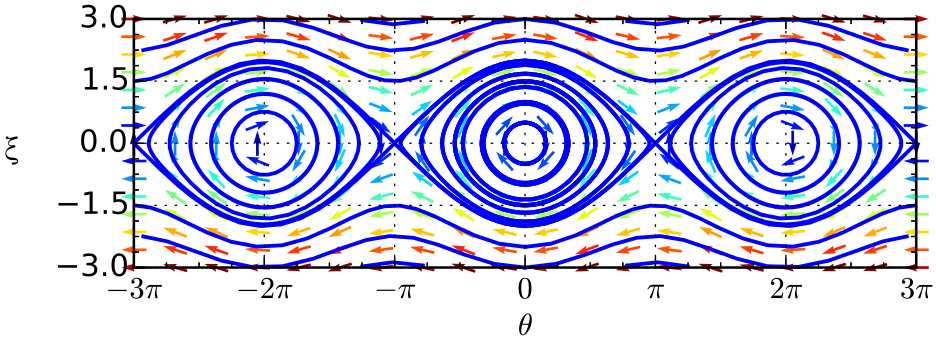
\includegraphics[width=.85\textwidth]{figures/pendulum_phase_space.png}};
		\end{tikzpicture}
		\caption{}
		\label{fig:pendulum_phase_diagram}
	\end{figure}

	The critical points of $h$ can be read from the expression of $dh$: $\xi d\xi + \sin \theta d\theta$, and are
	\begin{eqalign}
		\xi = 0, \quad \theta = 0,\, \pm \pi
	\end{eqalign}
	Due to these points, the system is not integrable (as $dh = 0$ implies $X_h =0$, i.e. the distribution described by $X_h$ is not smooth, see Construction~\ref{const:compl_integr_Ham_system}), so we remove them from the manifold $M$. In this new manifold, which is again symplectic and smooth, the system is everywhere integrable and its integral submanifolds are either circles (for closed orbits) or copies of $\R$ (for the extremal orbit which is a circle with two points removed, as well as for larger orbits which are unaffected).
\end{example}

It is somewhat surprising that the fibration phenomenon we have seen at the end of Example~\ref{ex:pendulum} is not peculiar to that example: \textbf{integral submanifolds happen to be always tori or Euclidean spaces}. This is the subject of Arnold--Liouville Theorem.

We start with a construction and some vocabulary:

\begin{construction}
\label{const:level_submanifolds_of_involutions}
	Let $(M, \omega)$ be a $2n$-dimensional symplectic manifold, let $h_1, \ldots, h_n$ be functions in involution and let finally $c \in \R^n$ be a regular value of
	\begin{eqalign}
		H : M &\longto \R^n\\
		p &\longmapsto (h_1(p), \ldots, h_n(p))
	\end{eqalign}
	meaning that $dh_1\vert_p, \ldots dh_n \vert_p$ are linearly independent at each $p \in H^{-1}(c)$.

	By the inverse function theorem\footnote{Theorem 2.4.23 \cite{abate2011geometria}.}, \textbf{$H^{-1}(c)$ is a submanifold of $M$ and its tangent spaces are generated by the Hamiltonian vector fields associated to the functions $h_1, \ldots, h_n$}: indeed,
	\begin{eqalign}
		T_pH^{-1}(c) = \ker dH_p = \{ X_p \in T_pM \suchthat X_p(h_i)=0\ \forall i \leq n \}
	\end{eqalign}
	and
	\begin{eqalign}
		X_{h_i}(h_j) = \omega(X_{h_i}, X_{h_j}) = \{ h_i, h_j \} = 0
	\end{eqalign}
	and the $X_{h_i}$ are independent. Moreover, \textbf{this computation also shows $H^{-1}(c)$ is a Lagrangian submanifold of $M$}, since it has dimension $n$ and $\omega$ vanishes on its generators.
\end{construction}

\begin{definition}
	Let $M$ be a symplectic manifold. A \textbf{Lagrangian fibration} is a submersion\footnotemark $H : M \to N$ where all of the fibres are Lagrangian submanifolds (a Lagrangian fibration is obviously a surjective submersion).
\end{definition}
\footnotetext{A submersion $H : M \to N$ is a smooth function such that $dH$ is pointwise surjective.}

\begin{remark}
\label{rem:submersion_to_Lag_fibration} 
	Let $H : M \to N$ be a submersion, $M$ symplectic, then the set $\operatorname{crit} H$ of critical points of $H$ is given by the vanishing of $\det dH$, hence it is closed. Then if all fibres of regular points of $H$ are Lagrangian submanifolds of $M$, we can promote $H$ to a Lagrangian fibration by restricting $M$ to the open set $M \setminus \operatorname{crit} H$.
\end{remark}

\begin{remark}
	Let $H : M \to \R^n$ as in Construction \ref{const:level_submanifolds_of_involutions}, then $H : M \setminus \operatorname{crit} H \to \R^n$ is a Lagrangian fibration.
\end{remark}

\begin{definition}
	A \textbf{locally trivial surjective submersion} is a surjective submersion $f: M \to N$ such that there exists a manifold $F$ and for every point $p \in N$ there exists an open neighbourhood $U$ of $p$ and a diffeomorphism $f^{-1}(U) \isoto U \times F$ which makes the following commute:
	\begin{diagram}
		M \arrow[relation=\supset]{r} \&[-3ex] f^{-1}(U) \arrow[swap]{dr}{f} \arrow{rr}{\phi} \& \& U \times F \arrow{dl}{\pr_1}\\
		\& \& U
	\end{diagram}
\end{definition}

\begin{definition}
	A \textbf{proper map} $f: X \to Y$, where $X$ and $Y$ are topological spaces, is a continuous map such that $f^{-1}$ maps compact sets to compact sets.
\end{definition}

\begin{lemma}[{\cite{mo2019properness}}]
\label{lemma:subm_is_proper}
	Any surjective submersion with compact and connected fibers is proper.
\end{lemma}

\begin{lemma}[Ehresmann]
\label{lemma:ehresmann}
	Any proper surjective submersion is locally trivial.
\end{lemma}

\begin{theorem}[Arnold--Liouville]
\label{th:arnold_liouville}
	Let $(M, \omega)$ be a $2n$-dimensional symplectic manifold equipped with $h_1, \ldots, h_n \in \Cinfty(M)$ functions in involution and define $H = (h_1, \ldots, h_n): M \to \R^n$. Suppose $H$ is a Lagrangian fibration.\footnote{We can always restrict to this case by removing the set of critical points of $H$ from $M$.} Let $p \in M$ such that the flows of $X_{h_1}, \ldots, X_{h_n}$, starting at $p$, are complete\footnotemark, and call $F^{(p)}$ the connected component of $H^{-1}(H(p))$ containing $p$. Then
	\begin{enumerate}
		\item $F^{(p)}$ is diffeomorphic to $\R^{n-k} \times \T^k$ for some $0 \leq k \leq n$ through a diffeomorphism that maps the flows of $X_{h_1}, \ldots, X_{h_n}$ to linear flows on $\R^{n-k} \times \T^k$; i.e. a linear $\R^n$-action on $\R^{n-k} \times \T^k$;
		\item in a neighbourhood of $F^{(p)}$ the functions $h_1, \ldots, h_n$ can be completed to a system of Darboux coordinates;
		\item the locus $M_C$ of all compact connected components of all fibers of $H$ is open in $M$, and $H\vert_{M_C}$ is a locally trivial Lagrangian fibration with fiber $\T^n$;
		\item in a neighbourhood of each fiber of $H\vert_{M_C}$ there exists a system of Darboux coordinates formed by $n$ angle variables on $\T^n$ and $n$ integrals of motion called \textbf{action variables} (where the term \emph{action} comes from their physical meaning).
	\end{enumerate}
	\footnotetext{A flow $\phi_t : M \to M$ is said \textbf{complete} if it is defined for any value of $t \in \R$, or --- equivalently --- that it is infinitely prolongable. This is always the case when $M$ is compact. Nevertheless notice that this requirement is not obvious if we defined the manifold $M$ by removing from it the set of all singular points, as the resulting manifold is open in the initial one.}
\end{theorem}
\begin{remark}
	The statement of \textbf{the theorem is agnostic about the choice of Hamiltonian function}. Indeed, it is not about Hamiltonian manifolds but about symplectic ones with $n$ functions in involution. Basically, this comes from the fact that the choice of $h$ is (from the mathematical point of view) arbitrary, since it comes from the physical situation: the mathematical content of the Hamiltonian formalism is given solely by the set of functions in involution.
\end{remark}
\begin{remark}
	To state the theorem globally (since any local statement about a symplectic manifold is trivial) we must ask for completeness of the flow. Indeed, to get fibers diffeomorphic to $\R$ and $\T^1$ we need complete flow lines.
\end{remark}
\begin{remark}
	The fourth statement only makes sense because of the previous one, otherwise there wouldn't be a way to extend the angle variables on a fiber to the neighboring ones. Moreover, in general the action variables will be a ``straightened-up'' version of the integrals of motions, hence not the same.
\end{remark}
\begin{proof}
	\leavevmode
	\begin{enumerate}
		\item We use the $1$-parameter diffeomorphism groups $\phi^{X_{h_1}}_t, \ldots, \phi^{X_{h_n}}_t$ of the given vector fields $X_{h_1}, \ldots, X_{h_n}$ to build an action\footnote{An action of a group $G$ on the set $M$ is an homomorphism of groups $f:G \to \Aut M$, i.e. an assignment of permutations of $M$ to elements of $G$, such that $f(gh) = f(g) \circ f(h)$ for every $g,h \in G$.} of $\R^n$ on $F^{(p)}$ by defining
		\begin{eqalign}
			\phi_{(t^1, \ldots, t^n)}(x) = \phi^{X_{h_1}}_{t^1} \circ \ldots \circ \phi^{X_{h_n}}_{t^n}, \quad \forall x \in F^{(p)}
		\end{eqalign}
		It is well-defined (as a group action) by virtue of the commutativity of the flows, which they inherit from their vector fields:
		\begin{eqalign}
			\phi_{(t^1+s^1, \ldots, t^n+s^n)}(x) &= \phi^{X_{h_1}}_{t^1+s^1} \circ \ldots \circ \phi^{X_{h_n}}_{t^n+s^n}\\
			&= \phi^{X_{h_1}}_{t^1} \circ \phi^{X_{h_1}}_{s^1} \circ \ldots \circ \phi^{X_{h_n}}_{t^n} \circ \phi^{X_{h_n}}_{s^n}\\
			&= \phi^{X_{h_1}}_{t^1} \circ \ldots \circ \phi^{X_{h_n}}_{t^n} \circ \phi^{X_{h_1}}_{s^1} \circ \ldots \circ \phi^{X_{h_n}}_{s^n}.
		\end{eqalign}
		Moreover, it is a transitive\footnote{An action of a group $G$ on the set $M$ is \textbf{transitive} iff for every pair of points $p, q \in M$, there is a $g \in G$ whose action brings $p$ to $q$.} action by the following argument. It's easy to see each point $x \in F^{(p)}$ has an open neighbourhood on which the flows, starting from $x$ itself, define a chart. This is true because\footnote{Theorem 3.7.4 \cite{abate2011geometria}.} $X_{h_1}, \ldots, X_{h_n}$ provide a basis for $T_xF^{(p)}$ made of independent and Lie-commuting vector fields. To show transitivity, we need to show any two $x,y \in F^{(p)}$ can be linked by flow lines. So pick a curve in $F^{(p)}$ connecting $x$ and $y$ (it exists since $F^{(p)}$ is connected by assumption). By compactness of the curve, a finite number of the charts we defined using the flows suffice to cover the whole path from $x$ and $y$, and we can assume the chart centered at $x$ and the one centered at $y$ to be in the covering. Now starting at $x$, follow the flow lines until they meet a point in the next chart, and then pick up another flow line of the second chart from there, and so on until we reach $y$. Clearly this defines a single segment of a flow line linking $x$ to $y$, implying $\phi$ is transitive.

		We then notice that, locally around any point, the action is free\footnote{An action of a group $G$ on the set $M$ is \textbf{free} if the identity of $G$ is the only element inducing the identity on $M$.} (indeed, as we already observed, each point is the center of a chart given by the flows) meaning the stabilizer of any point is a discrete subgroup of $\R^n$. Such a subgroup, we'll call it $\Gamma$, does not depend on the point we chose on $F^{(p)}$ (we can show this using transitivity of $\phi$ and abelianity of $\R^n$). Moreover, a discrete subgroup for $\R^n$ can only be a lattice of points generated by integer multiples of a family of $k$ independent vectors of $\R^n$. This suggests $\R^n / \Gamma \iso \R^{n-k} \times \T^k$. Moreover, this isomorphism of groups is also a \emph{diffeo}morphism as $\Gamma$ is a closed Lie subgroup of $\R^n$. The action $\phi$ then prolongs this diffeomorphism to $F^{(p)}$, proving the claim.

		\item So now we know that $F^{(p)} \iso \R^{n-k} \times \T^k$ and by definition $h_1, \ldots, h_n$ are constant on $F^{(p)}$. Since their differentials are linearly independent, they define a system of coordinates on the cotangent space of each fiber. Then we can use the $h_1, \ldots, h_n$ to move across fibers, and we will show that together with $t^1, \ldots, t^n$ (the flow times) they form a system of Darboux coordinates for a suitable choice of starting points for the flows on each fiber $H^{-1}(c)$ in a neighbourhood of $F^{(p)}$.

		Let us restrict to a tubular neighbourhood of $F^{(p)}$ where, since $F^{(p)}$ is Lagrangian (by Construction~\ref{const:level_submanifolds_of_involutions}), we have $\omega = d\eta$ for some $1$-form $\eta$ defined on such a neighbourhood (since tubular neighbourhoods inherit cohomology (Equation eq~\eqref{eq:tub_nbh_inherit_cohom}), see Proposition 6.8 \cite{daSilva2006}).

		Start by making an arbitrary choice of starting points for the flows. Then flows span an $n$-dimensional submanifold of the tubular neighbourhoods, which is transverse (i.e., the tangent spaces are never parallel) to each fiber $H^{-1}(c)$. The $t^1, \ldots, t^n, h_1, \ldots, h_n$ form a system of coordinates for the tubular neighbourhood. Let us compute the components of $\omega$ in such a system:
		\begin{eqalign}
			\omega(\partial_{t^i}, \partial_{t^j}) &= \omega(X_{h_i}, X_{h_j}) = \{h_i, h_j\} = 0\\
			\omega(\partial_{t^i}, \partial_{h_j}) &= \langle \ipr{X_{h_i}}\omega, \partial_{h_j} \rangle = \langle dh_i, \partial_{h_j} \rangle = \delta^j_i\\
			\omega(\partial_{h_i}, \partial_{h_j}) &=: V^{ij} \in \Cinfty(U).
		\end{eqalign}
		Hence we can write
		\begin{eqalign}
		\label{eq:omega_in_components}
			\omega = dt^i \wedge dh_i + V^{ij} dh_i \wedge dh_j.
		\end{eqalign}
		To get Darboux coordinates we want to eliminate the second term. Let's use the freedom of starting points to make the $V^{ij}$ vanish at $p$. Now, since $t^1, \ldots, t^n$ commute, $\Lie{\partial_{t^i}}dt^j = 0$,  and likewise $\Lie{\partial_{t^i}}dh_j = 0$.\footnote{Recall either Equation eq.~\eqref{eq:Lie_deriv_k_form} or Cartan's magic formula to compute explicitly these Lie derivatives.} Also $\Lie{\partial_{t^i}} \omega = 0$ by Theorem~\ref{th:flow_of_symp_field}. Hence, for each $k=1,\ldots, n$,
		\begin{eqalign}
			\pder{V^{ij}}{t^k} = \Lie{\partial_{t^k}}V^{ij} = \Lie{\partial_{t^k}} \omega(\partial_{h_i}, \partial_{h_j}) = 0
		\end{eqalign}
		meaning $V^{ij} = V^{ij}(h_1, \ldots, h_n)$, that is, \textbf{they only depend on the transverse coordinates}. On the other hand, in the tubular neighbourhood we are working in, $\omega$ is an exact form. Moreover, so is its first term (from \eqref{eq:omega_in_components}):
		\begin{eqalign}
			dt^i \wedge dh_i = d(t^i dh_i).
		\end{eqalign}
		Hence we impose $V^{ij} dh_i \wedge dh_j$ to be exact, which means the second term has to be the differential of some $1$-form $W$ depending only on $h_1, \ldots, h_n$, which implies that
		\begin{eqalign}
			V^{ij} = \partial_{h_j} W^i - \partial_{h_i} W^j.
		\end{eqalign}
		Then
		\begin{eqalign}
			\omega = d(t^i dh_i + W^i dh_i) = d(t^i + W^i) \wedge dh_i.
		\end{eqalign}
		By defining new coordinates $\tilde{t}^i = t^i + W^i(h_1, \ldots, h_n)$, it's clear we get a Darboux system. Since the $W^i$s depend only on the integral of motions, these new coordinates are still ``times'' for the flows but considered with a different starting point, as stated initially.

		\item Can we say something more when fibers are compact? Are they ``common'' or do they appear isolated? We'll show they form open sets in $M$. Let $M_C$ be the union of all compact connected components of any fiber. We claim $M_C$ is open in $M$.

		Suppose $M_C$ is not open. Then $M \setminus M_C$ is not closed, so that not all sequences of points $\seq{p}{i} \subseteq M \setminus M_C$ and converging in $M$ converge in $M \setminus M_C$. This means we can select one of those, such that $p_i \conv p \in M_C$ while $p_i \in M \setminus M_C$ for all $i \in \N$. Let $U$ be an open neighbourhood of $K^{(p)}$ (the compact connected component of $H^{-1}(H(p))$ containing $p$) such that $\closure U$ is compact and small enough as to not intersect other connected components of the same fiber $H^{-1}(H(p))$. For $i$ large enough, $(\closure U \setminus U) \cap F^{(p_i)} = \varnothing$: indeed, if it were otherwise, we could choose points $p'_i$ in each intersection $(\closure U \setminus U) \cap F^{(p_i)}$ and from those it can be selected a converging subsequence $\subseq{p'}{i}{k}$ by virtue of compactness of $\closure U \setminus U$ (it is closed in a compact). Let $p' \in \closure U \setminus U$ be the limit point of the subsequence. Since the two subsequences come from the same fibers, $H(p'_{i_k}) = H(p_{i_k})\ \forall k$. Using continuity of $H$, we obtain $H(p') = H(p)$, implying $p' \in K^{(p)}$, contradicting the assumption that $K^{(p)}$ doesn't intersect the boundary of $U$. So $F^{(p_i)} \cap (\closure U \setminus U) = \varnothing$ which implies (since the $p_i$ accumulate on $p$)
		\begin{eqalign}
			F^{(p_i)} \subseteq U \quad \forall \text{$i$ large enough}.
		\end{eqalign}
		Since $F^{(p_i)}$ is closed (since it's the preimage of $H(p_i)$, closed) and contained in $\closure U$, meaning it is compact itself. Moreover, $p_i \in M_C$, a contradiction with their definition. Thus $M_C$ is open, hence a (sub)manifold (of $M$). Apply now Lemma~\ref{lemma:subm_is_proper} and Ehresmann's Lemma (\ref{lemma:ehresmann}) in succession to the map $H$ on $M_C$ to conclude the proof.

		\item Since ${H: M_C \to \R^n}$ is locally trivial, we can identify a neighbourhood of each fiber with $U_0 \times \T^n$ and $U_0 \subseteq \R^n$ is open ($H$ is a fibration in tori). By point (2), $\omega = d(t^i dh_i) = -d(h_i dt^i)$ where $h_1, \ldots, h_n$ are linear coordinates on $\R^n$ and $t^1, \ldots, t^n$ are linear functions on $\T^n$. What we want to do now is a change of coordinates to get angle coordinates on the torus. Since we'd like this change to be structure-preserving, we'll try to get it as a canonical transformation, thus a symplectomorphism found through a generating function.

		Start by choosing a basis $\gamma_1, \ldots, \gamma_n \in H_1(\T^n)$, hence smooth circles around each factor of $\T^n$. Now define\footnote{Notice that these functions do not depend on the representatives $\gamma_\alpha$ of the homology classes we chosen, indeed for any equivalent loop $\gamma'_\alpha$ we have 
		\begin{eqalign}
			-\int_{\gamma_\alpha} h_i \, dt^i + \int_{\gamma'_\alpha} h_i \, dt^i = -\int_{M_\alpha} d(h_i \, dt^i) =  \int_{M_\alpha} \omega = 0
		\end{eqalign}
		where $M_\alpha$ is a submanifold of $\T^n$ whose border is given by $\gamma_\alpha$ and $\gamma'_\alpha$. The last step follows from $\omega\vert_{\T^n}=0$.}
		\begin{eqalign}
			I_\alpha(h_1, \ldots, h_n) := -\int_{\gamma_\alpha} h_i \, dt^i,
		\end{eqalign}
		Since $H$ is constant on each $\gamma_\alpha$, the $h_i$ in the integral are (non-zero) constants, so that the assignment is a linear function:
		\begin{eqalign}
			(I_\alpha) = \underbrace{(-\int_{\gamma_\alpha} \,dt^i)}_A (h^i).
		\end{eqalign}
		Since we choose $\gamma_1, \ldots, \gamma_n$ to be linearly independent, the matrix $A$ can be easily shown to be invertible. Then we can write:
		\begin{eqalign}
			h_\alpha = h_\alpha(I_1, \ldots, I_n).
		\end{eqalign}
		Now define
		\begin{eqalign}
			S(I_1, \ldots, I_n, t^1, \ldots, t^n) := - \sum_{i = 1}^n \int^{t^i}_{0} h_i(I_1, \ldots, I_n) \, dt.
		\end{eqalign}
		Again, the integral is performed along a curve where $I_\alpha$ are constants. Then by definition $h_\alpha = -\partial S / \partial t_\alpha$, thus calling $\phi^\alpha = \partial S / I_\alpha$ we get a canonical transformation whose generating function is $S$ such that
		\begin{eqalign}
			\omega = dt^i \wedge dh_j = d\phi^\alpha \wedge dI_\alpha.
		\end{eqalign}
		Moreover, these second set of coordinates are the angle coordinates we were looking for. Indeed, fix a $\beta$:
		\begin{eqalign}
			\phi^\alpha(p + \gamma_\beta) &= \pder{}{I_\alpha} \left( - \sum_{i = 1}^n \int^{t^i(p+\gamma_\beta)}_{0} h_i(I_1, \ldots, I_n) \, dt \right)\\
			&= \pder{}{I_\alpha} \left( - \sum_{i = 1}^n \int^{t^i(p)}_{0} h_i(I_1, \ldots, I_n) \, dt  - \int_{\gamma_\beta} h_i(I_1, \ldots, I_n) \, dt^i \right)\\
			&= \pder{}{I_\alpha} (S(I_1, \ldots, I_n, t^1(p), \ldots, t^n(p)) - I_\beta)\\
			&= \phi^\alpha(p) - \delta^\alpha_\beta.
		\end{eqalign}
		That shows $\phi^\alpha$ is a periodic function in the $\alpha$-th direction.
	\end{enumerate}
\end{proof}

\begin{remark}
	From the proof of the last point of the Arnold--Liouville theorem we see in particular that, given $n$ integrals of motion $h_1, \ldots, h_n$ and a basis $\gamma_1,\ldots, \gamma_n \in H_1(\T^n)$ of smoothly varying loops in the level set $\{h_\alpha (p) = h_\alpha\}$ the action variables $I_\alpha$ can be defined in a tubular neighbourhood of any fiber where $\omega = d\eta$ as
	\begin{eqalign}
		I_\alpha (h_1, \ldots, h_n) = \int_{\gamma_\alpha}\iota^*\eta
	\end{eqalign}
	where $\iota : \{h_\alpha(p) = h_\alpha\} \into M$ is the embedding of the level set into $M$. 
	
	Moreover, given any local system of Darboux coordinates $x^1, \ldots, x^n, \xi_1, \ldots, \xi_n$ with $\omega = d(x^i \, d\xi_i)$ where the manifolds $\{x^i = \text{const.}\}$ are transversal to the fibers $\{h_i = \text{const.}\}$, the equation
	\begin{eqalign}
		I_\alpha (x^1, \ldots, x^n, \xi_1, \ldots, \xi_n) = I_\alpha
	\end{eqalign}
	can be inverted to 
	\begin{eqalign}
		\xi_\alpha = \xi_\alpha(x^1, \ldots, x^n, I_1, \ldots, I_n).
	\end{eqalign}
	Then
	\begin{eqalign}
		S (x^1, \ldots, x^n, I_1, \ldots, I_n) = - \int^x_{x_0} \xi_\alpha (x, I) \, dx^\alpha
	\end{eqalign}
	where the integration is on any curve on $\{I_\alpha = \text{const.}\}$. The angle variables are hence
	\begin{eqalign}
		\phi^\alpha = \pder{S}{I_\alpha} ( x, I(x, \xi))
	\end{eqalign}
\end{remark}

\section{Applications of Arnold--Liouville Theorem}
\begin{example}[Simple pendulum]
	Let's analyze Example~\ref{ex:pendulum} in light of Arnold--Liouville Theorem. Figure~\ref{fig:pendulum_phase_diagram} shows the fibration induced by $h$ on $T^*S^1$. We need to take in consideration that the diagram should actually be wrapped around a cylinder. Hence not only the closed curves near the singular point $(0, 0)$ are compact fibers, but also the ones further away, which look open on the plane but close up on the cylinder. The open fibers are the two halves of the ``doubly punctured'' circle which constitutes the separatrix between the two families of compact fibers.

	\begin{figure}[H]
		\centering
		\begin{tikzpicture}
			\node (image) at (0,0) {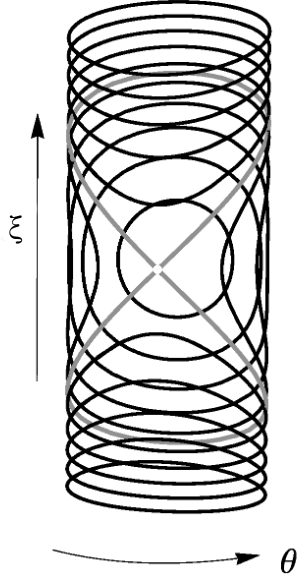
\includegraphics[width=.3\textwidth]{figures/pendulum_phase_space-cylinder.png}};
		\end{tikzpicture}
		\caption{The manifold $T^* S^1$, with compact fibers as solid black lines and open ones in grey.}
	\end{figure}
\end{example}

\begin{example}[Spherical pendulum]
	This time $M=T^*S^2$, we choose $\theta$ (longitude, $0 < \theta < 2\pi$) and $\phi$ (latitude, $0 < \phi < \pi$) as angle coordinates for $S^2$ and $\xi, \eta$ for the remaining ones. The Hamiltonian of the system is
	\begin{eqalign}
		h(\theta, \phi, \xi, \eta) = \frac12 \left(\eta^2 + \frac{\xi^2}{\sin^2\phi}\right) + \cos \phi
	\end{eqalign}
	whose differential is
	\begin{eqalign}
		dh = \eta d\eta + \frac{\xi}{\sin^2 \phi}d\xi - \left(\frac{\xi^2 \cos\phi}{\sin^3 \phi} + \sin\phi\right) d\phi
	\end{eqalign}
	which is singular iff $\eta=\xi=0$, $\phi=0,\pi$. Since $\dim S^2 = 2$, we need another integral of motion to apply Arnold--Liouville. Indeed, notice $h$ doesn't really depend on $\theta$! So we put $h_2=\xi$ ``$(=\dot \theta)$'' (check this commutes!).

	Let's check the points where $dh_1$ is not linearly indipendent from $dh_2$ (as with the singular points check for $dh$, this is in order to satisfy the hypothesis of Arnold--Liouville). As $dh_2 = d\xi$, this happens only when $dh_1$ has just the $d\xi$ term, i.e. the other two vanish:
	\begin{eqalign}
		\eta = 0, \quad \xi = \pm \sqrt{-\frac{\sin^4 \phi}{\cos \phi}}.
	\end{eqalign}
	Notice the condition on $\xi$ can be satisfied iff $\phi > \pi/2$ (since it is already less than $\pi$ by definition).

	On the singular points of $dh_1$, $X_{h_1} = X_{h_2} = 0$ (where the second equality is extended to the points outside the chosen chart by a simple continuity argument) while in the second set of points (where the differentials are not independent)
	\begin{eqalign}
		X_{h_1} &= \pm \frac1{\sqrt{-\cos\phi}} \partial_\theta\\
		X_{h_2} &= \partial_\theta
	\end{eqalign}
	The first case corresponds to the configurations where the pendulum is vertical, either upwards or downwards. The fact that the two Hamiltonian vector fields are zero tells us it has to stay still to maintain the balance. The second case represents circle orbits below the equator, those where gravity is balanced by centrifugal force.
\end{example}

\begin{exercise}
	Apply Arnold--Liouville Theorem to the ``updated'' phase space of the spherical pendulum, in particular describe the fibers of the Lagrangian fibration and the locus $M_C$ of the compact ones.
\end{exercise}

\begin{example}[$2$-species ``predator--prey'' Lotka--Volterra'' system]
	The \textbf{Lotka--Volterra model} describe predator-prey (or herbivore-plant, or parasitoid-host) dynamics in their simplest case (one predator population, one prey population). It was developed independently by Alfred Lotka and Vito Volterra in the 1920's, and is characterized by oscillations in the population size of both predator and prey, with the peak of the predator's oscillation lagging slightly behind the peak of the prey's oscillation. 
	
	The model makes several simplifying assumptions: 
	\begin{enumerate}
		\item the prey are assumed to have an unlimited food supply and to reproduce exponentially, unless subject to predation.; 
		\item the growth of predators population depend on the availability of food, the predator population will starve in the absence of the prey population (as opposed to switching to another type of prey) and in this case decreases exponentially; 
		\item predators can consume infinite quantities of prey; 
		\item there is no environmental complexity (in other words, both populations are moving randomly through a homogeneous environment).
	\end{enumerate}
	
	Given the following parameters describing the two populations and the interaction of the two species:
	\begin{enumerate}
		\item $P$ = number of predators or consumers;
		\item $p$ = number of prey or biomass of plants;
		\item $t$ = time;
		\item $m$ = predator death rate\footnote{Represents the loss rate of the predators due to either natural death or emigration, it leads to an exponential decay in the absence of prey.};
		\item $a$ = predator growth rate;
		\item $r$ = growth--death rate of prey (in absence of predators);
		\item $c$ = predation rate\footnote{Note the similarity to the predator growth rate; however, a different constant is used, as the rate at which the predator population grows is not necessarily equal to the rate at which it consumes the prey};
	\end{enumerate}
	then the populations change through time according to the pair of equations:
	\begin{eqalign}
	\label{eq:Lotka_Volterra_system}
		\begin{dcases}
			\der{P}{t} = - mP + aPp\\
			\der{p}{t} = rp-cPp
		\end{dcases}
	\end{eqalign}
	Consider the Hamiltonian system $(M, \omega, h)$ such that
	\begin{eqalign}
		M = \R^2_{>0} \qquad \omega^{-1} = Pp \pder{}{P} \wedge \pder{}{p} \qquad h(P,p) = - ap + m\log p - cP + r\log P
	\end{eqalign}
	with coordinates $P$, $p$ on $M$. The differential of the Hamiltonian is 
	\begin{equation}
		dh = (- cP + r) \frac {dP}{P} + (- ap + m) \frac {dp}{p}
	\end{equation}
	We see that using\footnote{Recall Remark \ref{eq:inv_sym_form_Ham_fields}. For $P$ we have $\dot P = \{P, h\} = \omega(X_P, X_h) = \omega^{-1}(dP, dh)$ which gives the first equation in eq.~\eqref{eq:Lotka_Volterra_system}. Same procedure for $p$ leads to the second equation in eq.~\eqref{eq:Lotka_Volterra_system}.} Equation eq.~\eqref{eq:evolution_f_flow_Xh} the flow of $X_h$ gives the Lotka-Volterra eq.~\eqref{eq:Lotka_Volterra_system}.
	The only singular point of $dh$ is $\left ( \frac {r}{c}, \frac{m}{a} \right)$, where $X_h$ vanish. 
	
	We plot the level sets of $h$\footnote{In the following link one can find the Mathematica code for plot these level set, with the possibility of change the parameters of the model: \url{https://it.wikitolearn.org/File:Lotka-Volterra.svg}.}:
	
	\begin{figure}[H]
		\centering
		\begin{tikzpicture}
			\node (image) at (0,0) {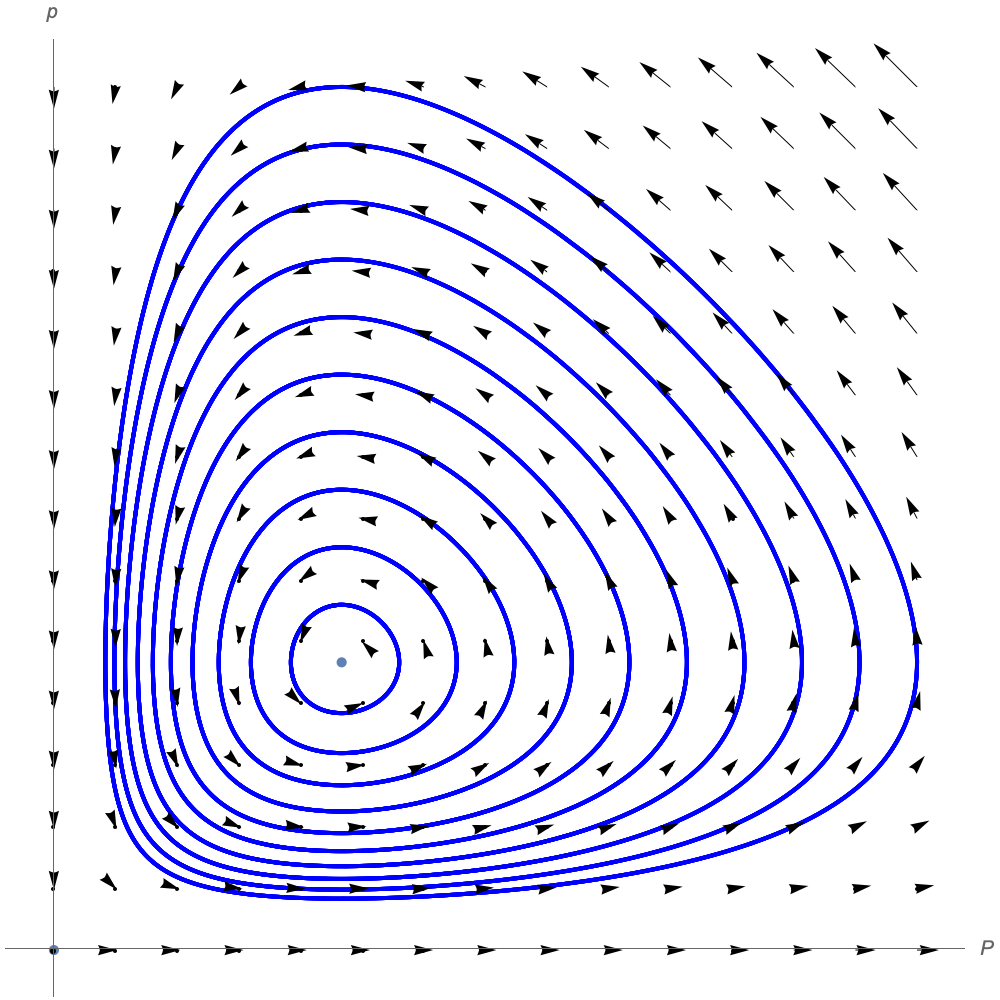
\includegraphics[width=.45\textwidth]{figures/Lotka_Volterra.png}};
		\end{tikzpicture}
		\caption{The manifold $\R^2_{>0}$, with compact fibers as solid blue lines, the blue point in the middle of the fibers is the equilibrium point. An extra equilibrium point outside the phase space is given by the origin of $\R^2$. Axis describe no prey (exponential decay of $P$) and no predator (exponential growth of $p$) cases.}
		\label{fig:Lotka_Volterra_diagram}
	\end{figure}
	
	There are some interesting special cases for this model. The first one is given by the case $m=0$, for instance if the predator can sustain its population even if there is no prey (e.g. it eats also vegetables). In such case the level sets of $h$ are:
	
	\begin{figure}[H]
		\centering
		\begin{tikzpicture}
			\node (image) at (0,0) {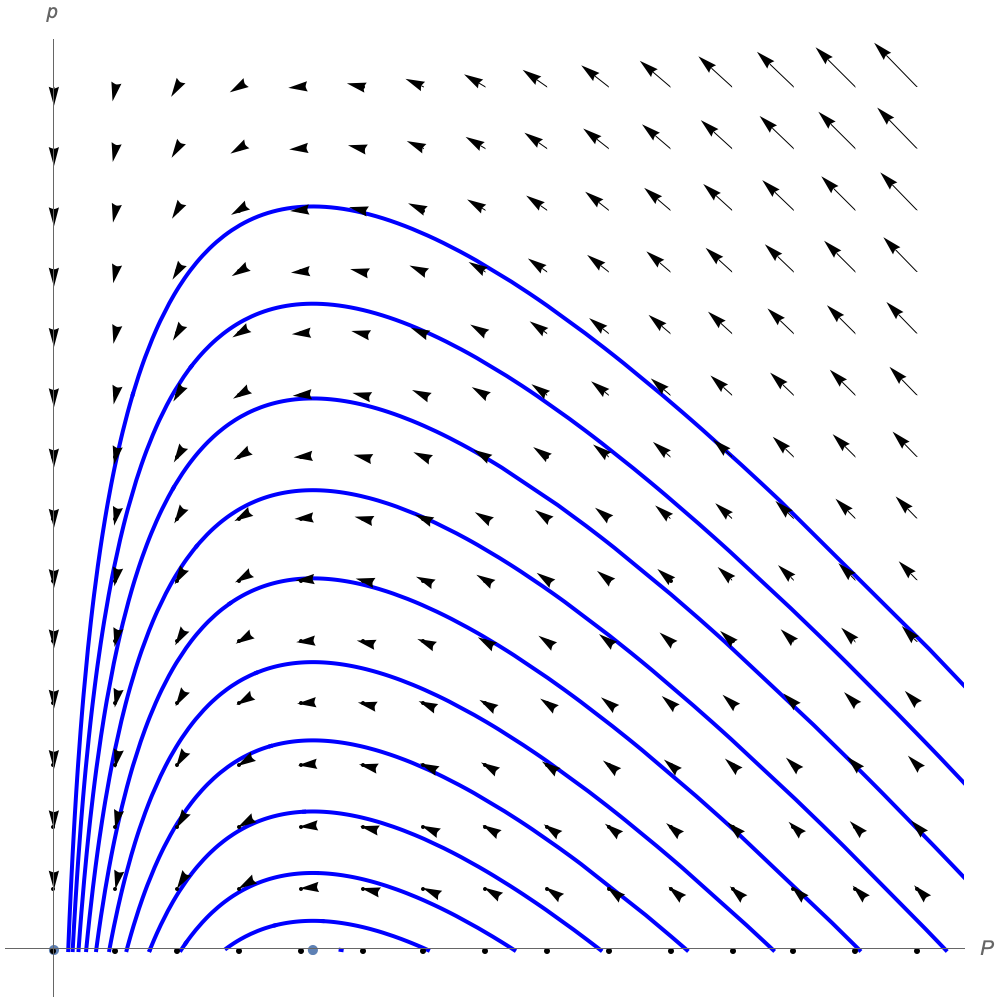
\includegraphics[width=.45\textwidth]{figures/Lotka_Volterra_SIR.png}};
		\end{tikzpicture}
		\caption{Special case $m=0$. In order to obtain the level sets shown in the picture one has to move slightly from the $P$-axis, in order to have a non-zero number of prey. The whole $P$-axis is corresponds to the case $\dot P = \dot p = p =0$, i.e. to the absence of prey and a constant number of predators. The blue point in the $P$-axis corresponds to the value $\frac{r}{c}$.}
		\label{fig:SIR_diagram}
	\end{figure}
	
	\noindent
	It's clear that in this case we have compact fibers provided that $a < 0$, otherwise the number of predators increases monotonically.
	
	Moreover, if we set $m=0$ and $a = c$  then Lotka--Volterra system eq.~\eqref{eq:Lotka_Volterra_system} becomes 
	\begin{eqalign}
	\label{eq:SIR_model_system}
		\begin{dcases}
			\der{P}{t} = -aPp\\
			\der{p}{t} = aPp-rp
		\end{dcases}
	\end{eqalign}
	where we changed the signs of parameters for convenience. When an individual of $P$ meets an individual of $p$ it becomes an individual of $p$ too with some \emph{contact rate} $a$, moreover the population $p$ decreases monotonically as $r$ is chosen positive. We can then interpret $P=S$ to be the population susceptible to some infection and $p=I$ to be the infected population. Then $a$ corresponds to the new infections per infected individual per day and $r$ is the fraction of infected that recover per day, i.e. $r^{-1}$ is the average duration of disease if we consider a uniform distribution, indeed if there are no new infected, the number of infected is described by $I(t) = \exp(-rt)$, and the average duration of the disease is then $\int_0^\infty I(t) dt = r^{-1}$. This leads to the \textbf{SIR model} (susceptible - infected - recovered) for the propagation of an infection in a population.\footnote{See \url{https://demonstrations.wolfram.com/SIREpidemicDynamics/} for some simulations of SIR model using Mathematica.} Figure fig.~\ref{fig:SIR_diagram} shows also the dynamic of this model. In this case the $P$-axis corresponds to the case where there are no infected and then the number of susceptible individuals is kept constant. 
\end{example}

\begin{example}[Kepler's problem on the plane]
	We assume that we already reduced the Kepler's problem from three dimensions to two dimensions by introducing the center of mass frame. Consider $M= T^*(\R^2 \setminus \{0\})$ with polar coordinates $r, \theta$ for the points and $p_r, p_\theta$ for covectors. The symplectic form on this manifold is
	\begin{eqalign}
		\omega = dr \wedge dp_r + d\theta \wedge dp_\theta
	\end{eqalign}
	along with Hamiltonian\footnote{We get this form from a suitable choice of description of the two-body system, from the reference frame of the center of mass.}
	\begin{eqalign}
		h = \frac{p^2_r}{2m} + \frac{p^2_\theta}{2mr^2} - \frac{k}{r}, \quad k,m > 0
	\end{eqalign}
	The two integrals of motion are then $h_1=h$ and $h_2 = p_\theta$.\footnote{This choice due to the fact that $h$ is independent from $\theta$, indeed using $X_{p_\theta} = \partial_\theta$ we obtain $\{h, p_\theta\} = \langle dh, X_{p_\theta} \rangle = 0$ and the two integral of motion are in involution.}

	As before, we now study the linear independence of $dh_1, dh_2$. First of all, they are
	\begin{eqalign}
		dh_1 &= \frac{p_r}m dp_r + \frac{p_\theta}{mr^2}dp_\theta + \left( \frac{k}{r^2} - \frac{p_\theta^2}{mr^3} \right)dr\\
		dh_2 &= dp_\theta
	\end{eqalign}
	thus they're indipendent unless
	\begin{eqalign}
		p_r = 0, \quad r = \frac{p_\theta^2}{mk}
	\end{eqalign}
	which correspond to particular circular orbits.

	To find the fibers, choose an arbitrary point $c = (c_1, c_2) \in \R^2$. Hence the equations of a level set of $H = (h_1, h_2)$ are
	\begin{eqalign}
	\label{eq:Kepler_level_set_eqs}
		\begin{dcases}
			c_1 = \frac{p_r^2}{2m} + V_{c_2}(r), \quad \text{where}\ V_{c_2}(r) = \frac{c_2^2}{2mr^2} - \frac{k}r\\
			c_2 = p_\theta
		\end{dcases}
	\end{eqalign}
	The term $V_{c_2}(r)$ is called the \emph{effective potential}. We then consider two cases.
	\begin{enumerate}
		\item $c_2 = 0$, yielding
		\begin{eqalign}
			c_1 = \frac{p_r^2}{2m} - \frac{k}r \implies r = \frac1k \frac1{\frac{p_r^2}{2m} - c_1}
		\end{eqalign}
		We observe that previous equation describes a non-compact curve in the $(r, p_r)$ plane, hence fibers of the form $H^{-1}(c_1, 0)$ correspond to unbounded orbits of the system and, geometrically, to non-compact fibers.\footnote{Notice that $\theta$ lives in $S^1$, so it never gives problems of compactness.}
		\item $c_2 \neq 0$, then inspecting the first equation we see that $c_1 < 0$ implies $V_{c_2}$ negative, thus when we draw its graph we notice in this case we have compact level sets (given by $r \in [r_-, r_+]$). Clearly, the level set is empty whenever $c_1 < \min V_{c_2}(r) = V_{c_2} \left(\frac{c_2^2}{mk} \right) =  - \frac{mk^2}{2 c_2^2}$.
		
		\vspace{-0.5cm}
		\begin{figure}[H]
			\centering
			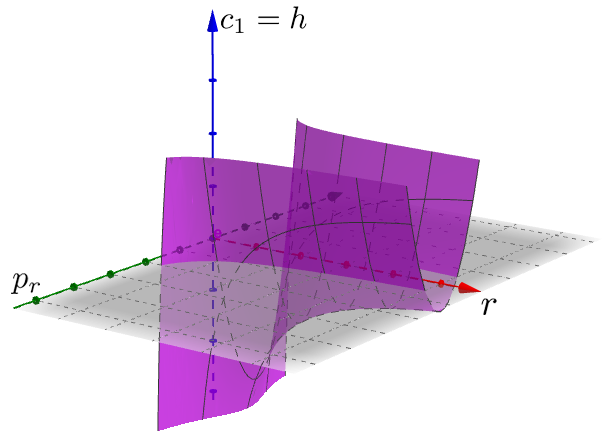
\includegraphics[width=.6\textwidth]{figures/Kepler_c2_0.png}
			\caption{Plot of first equation of eq.~\eqref{eq:Kepler_level_set_eqs} for $p_\theta = 0$, i.e. the body moves in the radial direction. Is clear that level sets $\{c_1 = \text{const.}\}$ are non-compact. For $h < 0$ level sets represent bounded states where the body is allowed to move away from the origin $r = 0$ only until a fixed value $r = r_+$. For $h \geq 0$  level sets represent states where the body has enough kinetic energy to leave definitely the original position.}
			\label{fig:Kepler_c2_0}
		\end{figure}
		\vspace{-0.5cm}
		\begin{figure}[H]
			\centering
			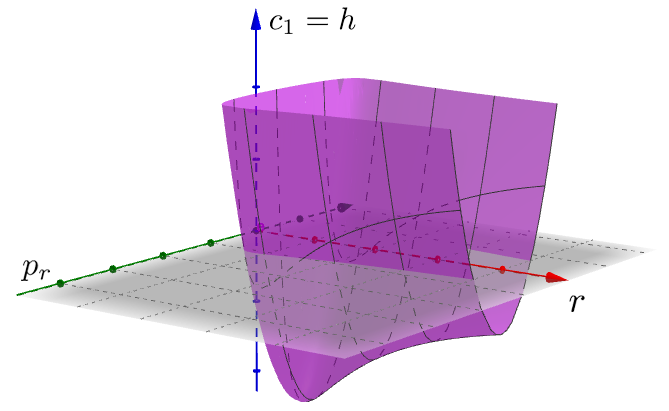
\includegraphics[width=.6\textwidth]{figures/Kepler_c2_neq_0.png}
			\caption{Plot of first equation of eq.~\eqref{eq:Kepler_level_set_eqs} for $p_\theta \neq 0$, i.e. the body moves with non-zero angular momentum. For $h = 0$ we have compact fibers where the body is bounded in the range $r \in [r_-, r_+]$, i.e. represent bodies with compact orbits around the origin, such as planets in the Solar System. Conversely, for $h > 0$, the body state is no more bounded, and represent bodies which has enough energy to leave the attraction given by the effective potential, such as bodies which go through the Solar System without being bounded in orbits around the Sun because of their high kinetic energy.}
			\label{fig:Kepler_c2_neq_0}
		\end{figure}
		\begin{figure}[H]
			\centering
			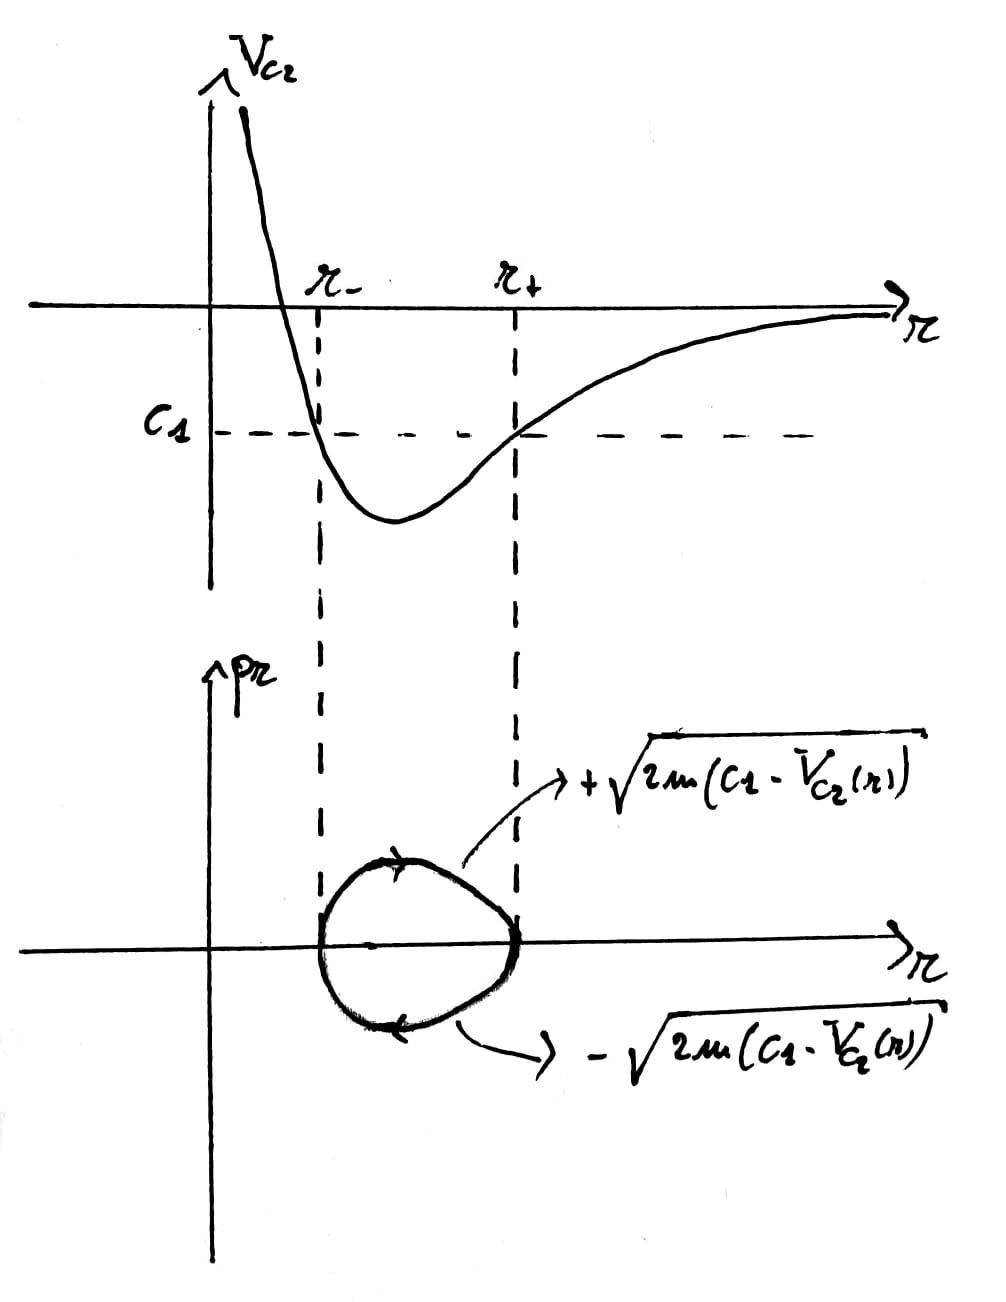
\includegraphics[width=.55\textwidth]{figures/KeplerCompactFiber.jpg}
			\caption{Level set given by $p_\theta \neq 0$ and $0 > h > -\frac{mk^2}{2c_2^2}$.}
			\label{fig:KeplerCompactFiber}
		\end{figure}
		\begin{figure}[H]
			\centering
			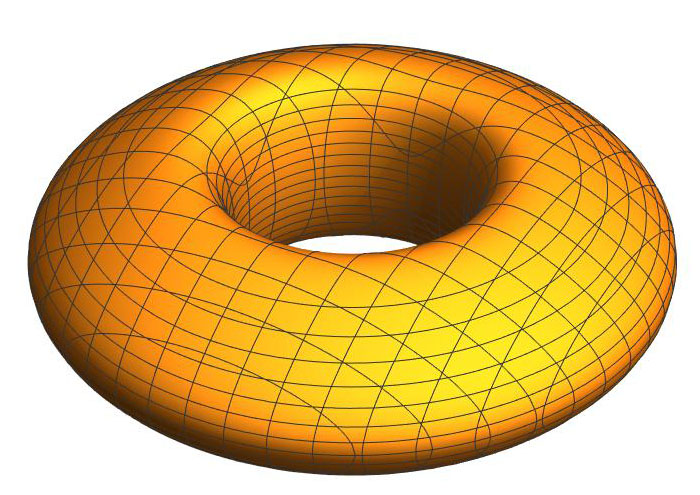
\includegraphics[width=.55\textwidth]{figures/Kepler_Lagrangian_fiber.jpeg}
			\caption{Once we fixed $c_1$ and $c_2$ in such a way to obtain a compact fiber as in Figure~\ref{fig:KeplerCompactFiber}, we can introduce the $\theta$ variable in our phase space obtaining the whole Lagrangian fiber through rotation of the second part of  Figure~\ref{fig:KeplerCompactFiber} for all $\theta \in [0, 2\pi)$.}
			\label{fig:KeplerLagrangianFiber}
		\end{figure}
		
	\end{enumerate}
	
	Therefore
	\begin{eqalign}
		H^{-1}(c_1, c_2) \begin{dcases}
			\text{is non-compact} = \R \times S^1 & \text{for $c_2 = 0$, $c_1 \geq 0$}\\
			= \T^2 & \text{when $c_2 \neq 0,\ - \frac{mk^2}{2c_2^2} < c_1 < 0$}\\
			= S^1 & \text{when $c_2 \neq 0,\ c_1 = -\frac{mk^2}{2c_2^2}$}\\
			= \varnothing & \text{when $c_2 \neq 0,\ c_1 < -\frac{mk^2}{2c_2^2}$}
		\end{dcases}
	\end{eqalign}
	Notice that the third case happens when $r= c_2^2/mk$, which we excluded previously for reasons of linear independence. Indeed, it represent a separatrix between compact and non-compact trajectories more or less like in the example of the pendulum. We can represent the fibration on the plane as such:

	\begin{figure}[H]
		\centering
		\begin{tikzpicture}
			\node (image) at (0,0) {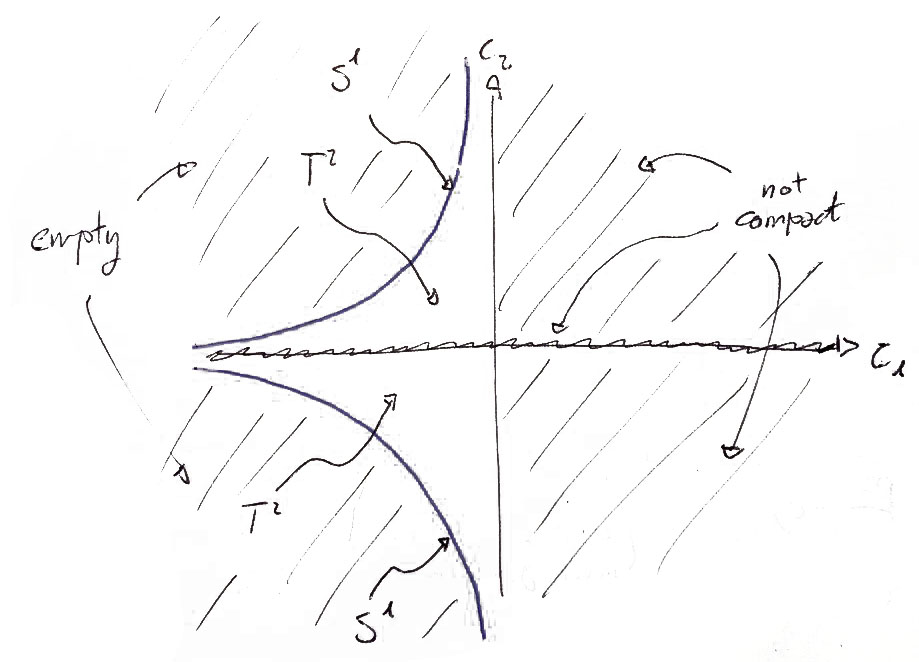
\includegraphics[width=.85\textwidth]{figures/Kepler_fibers.jpg}};
		\end{tikzpicture}
	\end{figure}

	Thus the region of the plane giving compact fibers (i.e. tori) is
	\begin{eqalign}
		B = \left\{ (h, p_\theta) \in \R^2 \suchthat h < 0,\ 0 < |p_\theta| < k \sqrt{-m/2h} \right\}
	\end{eqalign}
	We can now move on to find the action-angle variables of the system: we start choosing $\gamma_1, \gamma_2$ basis for $H_1(H^{-1}(c_1, c_2))$. As the first one, we choose the circle in the $\theta$ direction parametrized by
	\begin{eqalign}
		\gamma_1 : S^1 &\longto H^{-1}(c_1, c_2)\\
		t &\overset{\theta}\longmapsto \begin{dcases}
			\theta = t\\
			r = \frac{-k + \sqrt{k^2 + \frac{c_1c_2^2}{m}}}{2c_1}\\
			p_r = 0\\
			p_\theta = c_2
		\end{dcases}
	\end{eqalign}
	The expression for $r$ is computed by imposing the circle to stay inside the fiber $H^{-1}(c_1, c_2)$, once we fixed $p_r=0$ (which is an arbitrary choice).

	The other loop $\gamma_2$, independent from $\gamma_1$, is naturally sought in the complementary part $(r,p_r)$ of the fibers: as seen in Figure~\ref{fig:KeplerCompactFiber}, an $S^1$ is actually present (the disentanglement of the $r$-dynamics from the $\theta$-dynamics is due to the $\theta$-independence of $h$).

	\begin{figure}[H]
		\centering
		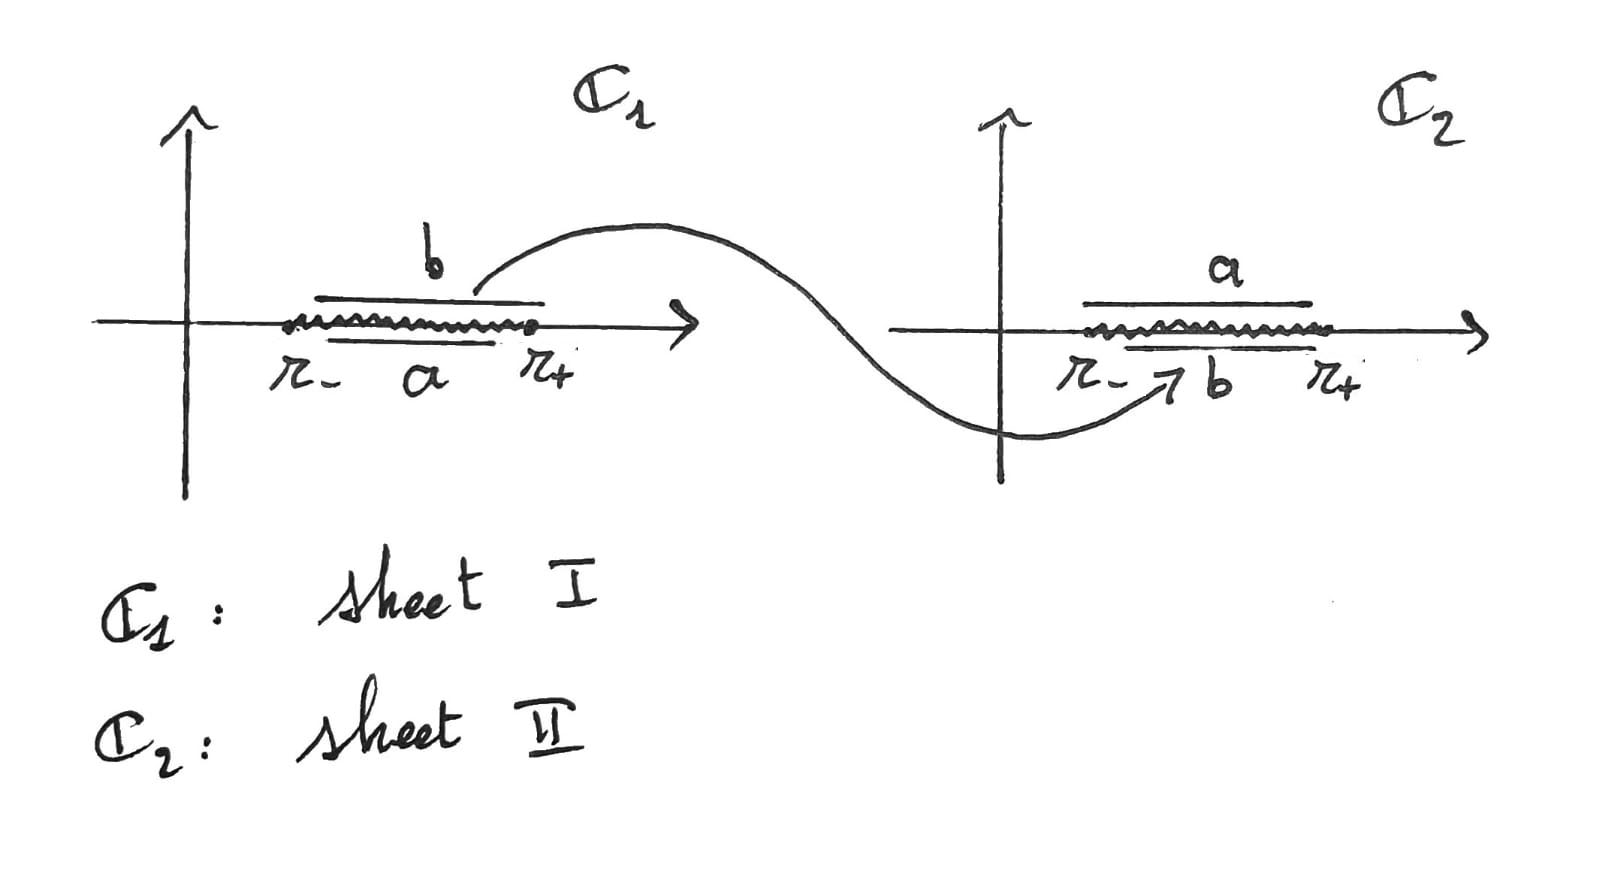
\includegraphics[width=.85\textwidth]{figures/MultivaluedFunctionDef.jpeg}
		\caption{}
		\label{fig:MultivaluedFunctionDef}
	\end{figure}

	Although harder to visualize, this should make clear why $\gamma_2$ can be chosen to be formed by two branches $\gamma^\pm_2$ stitched together at the ends:
	\begin{eqalign}
		\gamma_2^\pm : (r_+, r_-) &\longto H^{-1}(c_1, c_2)\\
		t &\longmapsto \begin{cases}
			\theta = 0 \comment{(arbitrary choice)} \\
			r= \pm t\\
			p_r = \pm \sqrt{2m \left(c_1 - V_{c_2}(\pm t) \right)}\\
			p_\theta = c_2
		\end{cases}
	\end{eqalign}
	The expression for $p_r$ is computed by imposing the circle to stay inside the fiber $H^{-1}(c_1, c_2)$, once we fixed $p_\theta=c_2$.
	The values $r_+$ and $r_-$ are given by the zeroes of the discriminant of $h_1=c_1$:
	\begin{eqalign}
	 r_\pm = \frac{-k \pm \sqrt{k^2 + \frac{c_1c_2^2}{m}}}{2c_1} \qquad (r_+<r_-).
	\end{eqalign}

	Put together, $\gamma_2$ goes go back and forth between $r_+$ and $r_-$ using the $p_r$ dimension.

	Then recall $\omega = d(-p_\theta d\theta - p_rdr)$, so, since $p_r=0$ on $\gamma_1$.
	\begin{eqalign}
		I_1(c_1, c_2) = - \int_{\gamma_1} (p_\theta d\theta + p_r dr) = -2\pi c_2
	\end{eqalign}
	As for computing $I_2$, $\gamma_2$ is obtained by spanning $r$ from $r_+$ to $r_-$ setting $p_r(r)=+g(r)$,
	and then spanning $r$ from $r_-$ to $r_+$ setting $p_r(r)=-g(r)$, where $g(r)=\sqrt{2m(c_1-V_{c_2}(r))}$, therefore
	\begin{eqalign}
		I_2(c_1, c_2) &= - \int_{\gamma_2} p_r dr \\
			      &= -\left(\int_{r_+}^{r_-} g(t) \,dt + \int_{r_-}^{r_+} (-g(t)) \,dt\right).
	\end{eqalign}
	To compute it, we use residues by interpreting the integral in the complex $t$ plane.

	In order to do that, we aim to rewrite $I_2$ as a circuit integral and then to deform the integration path using
	the properties of integrals of holomorphic functions.
	Let us start by defining the following function
	\begin{eqalign}
	 \pi_r(t)=\frac{\sqrt{-2mc_1}}{t}\sqrt{(t-r_-)(t-r_+)}.
	\end{eqalign}
	This is clearly a multivalued function on two sheets, I and II, with two branches.
	It displays only two ramification points in $r_\pm$, therefore we take the cut connecting them as shown in Figure~\ref{fig:MultivaluedFunctionDef}.
	Finally, it features a simple pole in zero, while being holomorphic elsewhere.

	Next, consider its restrictions to the real axis above and below the cut (respectively b and a sides): one easily gets
	\begin{eqalign}
	 \pi_r(t)_{|_b}&=ig(t)	\\
	 \pi_r(t)_{|_a}&=-ig(t)
	\end{eqalign}
	therefore one can consider the line integral
	\begin{equation}
	 I=\int_\gamma \pi_r(t)\,dt
	\end{equation}
	where $\gamma$ is the path shown in Figure~\ref{fig:IntPath}.

	\begin{figure}
	\centering
	\begin{minipage}{0.45\textwidth}
	\centering
	 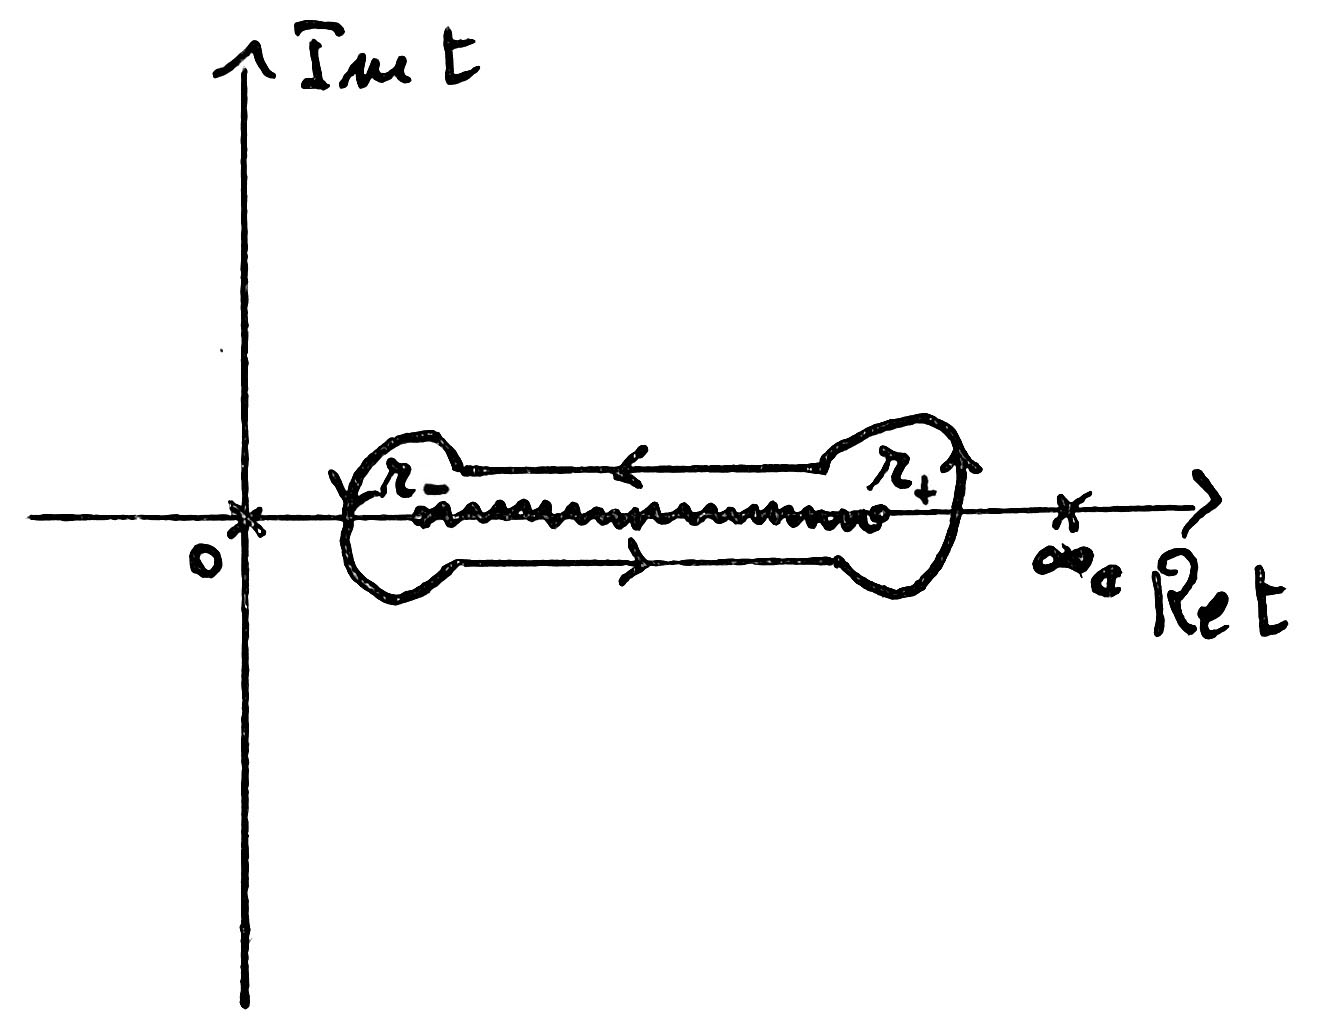
\includegraphics[width=\textwidth]{figures/IntPath.jpeg}
	 \captionof{figure}{}
	 \label{fig:IntPath}
	\end{minipage}
	\centering
	\begin{minipage}{0.5\textwidth}
	\centering
	 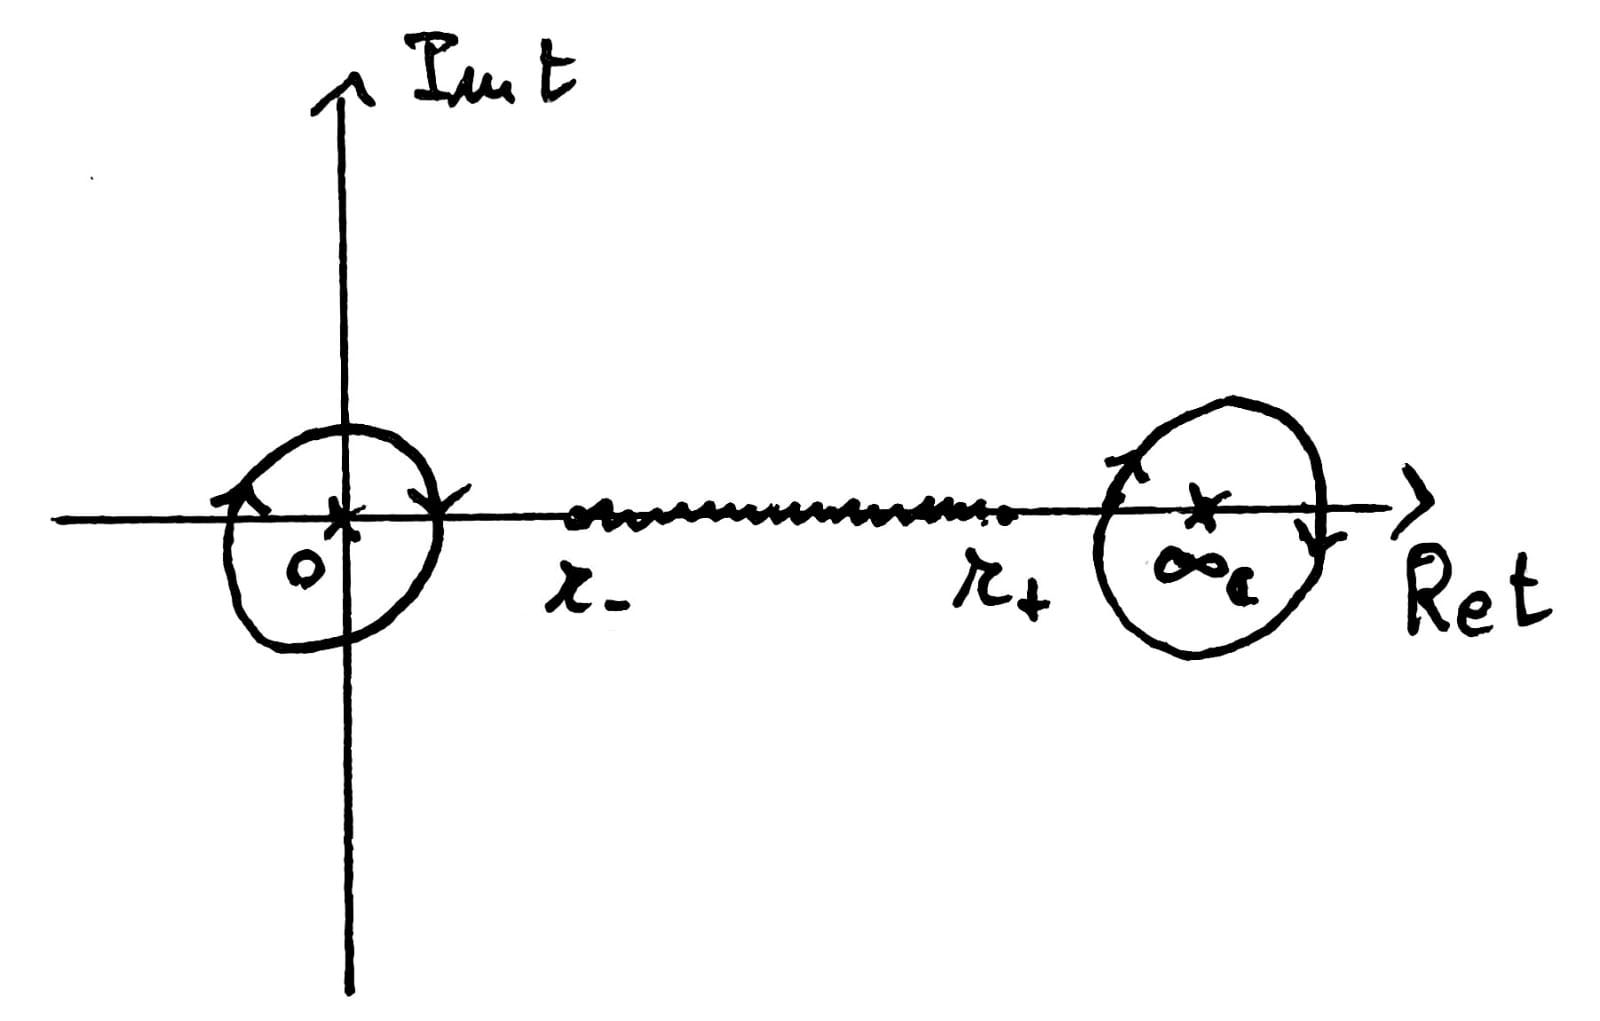
\includegraphics[width=\textwidth]{figures/ResidueIntPath.jpeg}
	 \captionof{figure}{}
	 \label{fig:ResidueIntPath}
	\end{minipage}
	\end{figure}

	One can continuously deform the integration path $\gamma$ without changing the result
	(since $\pi_r$ is holomorphic outside zero), so let us shrink $\gamma$ to the segment $[r_+,r_-]$, getting
	\begin{eqalign}
		I &=\int_{r_-}^{r_+}ig(x)\,dx+\int_{r_+}^{r_-}(-ig(x))\,dx\\
		  &=i\,I_2
	\end{eqalign}
	so that $I_2$ can actually be rewritten as
	\begin{equation}
		I_2(c_1,c_2)= -i\int_\gamma \pi_r(t)\,dt.
	\end{equation}

	Now we can use the residue theorem and trade $\gamma$ for the union of the circles $C_0$ and $C_\infty$ around
	the pole in zero and around $\infty_\C$ as integration path (see Figure~(\ref{fig:ResidueIntPath})).
	Keeping track of the inherited orientations of the circles, one gets
	\begin{eqalign}
	 I_2(c_1,c_2) &= \left(\int_{C_0} \pi_r(t) \,dt + \int_{C_\infty} \pi_r(t) \,dt\right)	\\
		      &= 2\pi i\left(-\underset{t=0}{\Res}(\pi_r(t))-\underset{t=\infty_\C}{\Res}(\pi_r(t))\right)
	\end{eqalign}

	Let us carry out the residue computation:
	\begin{enumerate}
	 \item \textbf{In $t=0$.} Let us expand $\pi_r$ in its Laurent series around $t=0$: one finds
			 \begin{equation}
			  \pi_r(t)=\frac{\sqrt{-2mc_1}}{t}\sqrt{r_+r_-}+\mathcal{O}(1),
			 \end{equation}
			 so that
			 \begin{eqalign}
			  \underset{t=0}{\Res}(\pi_r(t))&=\sqrt{-2mc_1r_+r_-}	\\
							&=c_2
			 \end{eqalign}
			 where we took $c_2>0$ and we used $r_+r_-=-\frac{c_2^2}{2mc_1}$.
	 \item \textbf{In $t=\infty_\C$.} Let us expand $\pi_r$ in its Laurent series around $t=\infty_\C$: one finds
			 \begin{equation}
			  \pi_r(t)=\sqrt{-2mc_1}-\frac{\sqrt{-2mc_1}(r_++r_-)}{2t}+\mathcal{O}(t^{-2}),
			 \end{equation}
			 therefore
			 \begin{eqalign}
			  \underset{t=\infty_\C}{\Res}(\pi_r(t))&=\frac{\sqrt{-2mc_1}}{2}(r_++r_-)	\\
							&=\frac{mk}{\sqrt{-2mc_1}}.
			 \end{eqalign}
	\end{enumerate}

	Finally, one gets
	\begin{eqalign}
	 I_2(c_1,c_2)&=-i\left[-2\pi i\Big(c_2+\frac{mk}{\sqrt{-2mc_1}}\Big)\right]	\\
		     &= -2\pi\left(c_2+\frac{mk}{\sqrt{-2mc_1}}\right).
	\end{eqalign}


	Reinserting back the functions for $c_1$ and $c_2$, one gets the following results:
	\begin{eqalign}
		I_1 &= -2\pi p_\theta\\
		I_2 &= -2\pi p_\theta - 2\pi \sqrt{\frac{mk^2}{-2 \left( \frac{p_r^2}{2m} + \frac{p_\theta^2}{2mr^2} - \frac{k}{r} \right)}}
	\end{eqalign}
	from which we can obtain the generalized momenta:
	\begin{eqalign}
		p_\theta &= -\frac1{2\pi} I_1\\
		p_r &= \sqrt{2m \left( -2\pi^2\frac{mk^2}{(I_2-I_1)^2} - \frac1{4\pi^2} \frac{I_1^2}{2mr^2} + \frac{k}{r} \right)}
	\end{eqalign}

	Call $\phi^\alpha$ the angle variables. Then
	\begin{eqalign}
		S(\theta, r, I_1, I_2) = \int_{(\phi_0, r_0)}^{(\theta, r)} (p_\theta d\theta + p_rdr)
	\end{eqalign}
	where the integration path is not relevant as long as it remains inside $H^{-1}(c_1, c_2)$. Then $\phi^\alpha = \partial S / \partial I_\alpha$, but \textbf{it's not possible to compute $S$ analytically}. However, we can still find the canonical transformation to get the action variables. We start by writing $h$ in terms of $I_1$ and $I_2$, an expression not depending on any other variable since $H$ is costant along the fibers. From the relative computation, we get
	\begin{eqalign}
		h=h(I_1, I_2) = 2\pi^2 \frac{mk^2}{(I_2 - I_1)^2}
	\end{eqalign}
	We know the equations of motion imply
	\begin{eqalign}
		\begin{dcases}
			\dot I_\alpha = 0 \comment{since it is an integral of motion}\\
			\dot\phi^\alpha = \pder{h}{I_\alpha} = \pm 4\pi^2 \frac{mk^2}{(I_2-I_1)^3}
		\end{dcases}
	\end{eqalign}
	Since $\phi^\alpha$ comes from the linear action on the torus, we can now get the angle coordinates:
	\begin{eqalign}
		\phi^\alpha = \dot\phi^\alpha t + \phi^\alpha_0
	\end{eqalign}

	The information we extracted from the system allows us, for example, to analyze the question of the periodicity of the motion. By computing the slope of the line described by the $\phi^\alpha$ on the toric fiber, we can answer positively that question:
	\begin{eqalign}
		\frac{\dot\phi^1}{\dot\phi^2} = -1 \in \Q
	\end{eqalign}
\end{example}

\begin{remark}
	The last part of the previous example shows an approach which works generally -- once we have $I_1, \ldots, I_n$, we can express $h$ in terms of them and then the angle variables as
	\begin{eqalign}
		\phi^\alpha = \pder{h(I_1, \ldots, I_n)}{I_\alpha} t + \phi^\alpha_0
	\end{eqalign}
\end{remark}

\end{document}
	\documentclass[main.tex]{subfiles}
\begin{document}

\chapter{Coadjoint orbits}
\section{The adjoint action of a Lie group}
A Lie group is a group supported on a smooth manifold and whose product and inverse maps are smooth. This is a very fertile combination of structures from which a canonical symplectic structure of certain associated manifolds (the \textbf{coadjoint orbits}) will emerge naturally. As Lie groups are a quite large class of manifolds which includes groups of matrices, such a treatment is relevant to many physical situations. Most of the topics treated in this chapter (actually most of the topics treated in these notes) are contained in \cite{michor2008}.

It is interesting to study the (smooth) actions of such a group, i.e. group maps
\begin{eqalign}
	\rho : G \times M \longto M
\end{eqalign}
where $M$ is a smooth manifold. Any such action, by virtue of the smooth structures involved, lifts by pushforward to an action on the fields
\begin{eqalign}
	\rho_* : G \times \fields(M) &\longto \fields(M)\\
		(g, X) &\longmapsto (\rho_g)_* X
\end{eqalign}
% We call \textbf{$\rho$-invariant} the fields on $M$ fixed by the latter action, and we designate them with $\fields^\rho(M)$. They form a Lie subalgebra of $\fields(M)$ since if $X,Y \in \fields^\rho(M)$, then for any $g \in G$ we have
% \begin{eqalign}
% 	(\rho_g)_*[X,Y] = [(\rho_g)_*X, (\rho_g)_*Y] = [X,Y].
% \end{eqalign}

Even when we do not have at our disposal another manifold $M$ for $G$ to act on, $G$ acts on itself already in interesting ways. The easiest way a group acts on itself is with the \textbf{left action}:
\begin{eqalign}
	L : G \times G &\longto G\\
	(g,h) &\longmapsto L_g(h) := gh
\end{eqalign}

A field $X \in \fields(G)$ is \textbf{left invariant} if $(L_g)_*X = X$ for all $g \in G$, i.e. $d(L_g)_x(X_x) = X_{gx}$ for all $g,x \in G$. We denote by $\fields^L(G)$ the set of all left invariant vector fields. 
One can prove\footnote{See \cite[Proposition 3.6.2]{abate2011geometria}.} that $\fields^L(G)$ is a Lie algebra with the usual bracket $[-,-]$ of vector fields. Moreover there is a Lie algebra isomorphism between $\fields^L(G)$ and $T_eG$:
\begin{eqalign}
	T_eG \underset{\cat{LieAlg}}\iso \fields^L(G) := \{X \in \fields(G) \suchthat (L_g)_* X = X\ \forall g \in G \}
\end{eqalign}
In fact, any vector in $T_e G$ can be extended to a left-invariant vector field by prolonging it using the action's flow, $X_g := d(L_g)_e(X_e)$; transitivity of $L$ takes care of injectivity issues. Evaluation at $e$ is the inverse map. The isomorphism induces a Lie algebra structure on $T_eG$, given by $[X_e, Y_e] := [X,Y]_e$, promoting the isomorphism to a Lie algebra isomorphism as claimed before. Both $T_eG$ and $\fields^L(G)$ are called the \textbf{Lie algebra} of $G$ and denoted by $\lalg$. 

Of course, these construction can be carried out for the \textbf{\emph{right} action}, too, defined obviosuly as multplication on the right. The fields invariant for this action are denoted by $\fields^R(G)$ and for the same reasons as before, they form a Lie algebra isomorphic to $T_e G$, thus to $\lalg$. However, this doesn't mean right-invariant fields are automatically left-invariant --- at all.

Since $\lalg$ can be considered a tangent space of $G$, to any action $\rho : G \times G \to G$ \emph{fixing the identity} (i.e. such that $\rho_g (e) = e$ for all $g \in G$) we can associate an action on the Lie algebra, simply by taking differentials at $e$:
\begin{eqalign}
	\mathfrak p : G \times \lalg &\longto \lalg\\
		(g, X_e) &\longmapsto d(\rho_g)_e(X_e)
\end{eqalign}

\begin{proposition}
	When $\rho : G \times G \to G$ is an action fixing the identity, then the action $\mathfrak p$ is isomorphic (in the representation-theoretic sense) to the pullback $\rho_*$ restricted to $\fields^L(G)$, that is, the following commutes for every $g \in G$:
	\begin{diagram}
		\fields^L(G) \arrow{r}{(\rho_g)_*} \arrow{d}{\phi} \& \fields^L(G) \arrow{d}{\phi}\\
		T_e G \arrow{r}{d\rho_g} \& T_e G
	\end{diagram}
	where $\phi$ is the isomorphism given by evaluation at $e$ discussed above.
\end{proposition}
\begin{proof}
	Let $X \in \fields^L(G)$, then
	\begin{eqalign}
		\phi((\rho_g)_*(X)) &= ((\rho_g)_*X)_e\\
		&= d(\rho_g)_{\rho_g^{-1}e}(X_{\rho_g^{-1}e})\\
		&= d(\rho_g)_e(X_e) \comment{because $\rho$ fixes $e \in G$}\\
		&= d\rho_g(\phi(X)).
	\end{eqalign}
\end{proof}

The simplest of such actions is the \textbf{conjugation action} (since the left action and the right action do not fix the identity):
\begin{eqalign}
	I : G \times G &\longto G\\
	(g, x) &\longmapsto I_g(x) := g x g^{-1}
\end{eqalign}
The identity $e \in G$ is a fixed point for this action.

Given $X\in\fields(G)$, we denote its associated flow by
\begin{eqalign}
	\phi^X_\bullet : (-\epsilon, \epsilon) \times G &\longto G\\
	(t, g) &\longmapsto \phi_t^X(g)
\end{eqalign}

\begin{definition}
	The \textbf{adjoint action} of a Lie group $G$ is the action
	\begin{eqalign}
		\Ad : G \times \lalg &\longto \lalg\\
		(g, X_e) &\longmapsto \Ad_g(X_e) := ((I_g)_* X)_e = \der{}{t}\vert_{t=0}(g\, \phi_t^X(e)\,g^{-1})
	\end{eqalign}
	induced on its Lie algebra $\lalg$ by the conjugate action, for any $X \in \fields^L(G)$.
\end{definition}

\begin{construction}
	If we are given a smooth action $\rho : G \times M \to M$ on a smooth manifold $M$, the flow through the identity $\phi^X_\bullet(e) : (-\epsilon, \epsilon) \to G$ induces a $1$-parameter group of diffeomorphisms of $M$:
	\begin{eqalign}
		\phi^{X_M}_\bullet : (-\epsilon, \epsilon) \times M &\longto M\\
		(t, p) &\longmapsto \rho_{\phi^X_t(e)}(p)
	\end{eqalign}
	Its derivative then defines a field\footnote{Usually in literature $X_M$ is called \textbf{fundamental vector field} associated with $X$.} $X_M \in \fields(M)$ such that
	\begin{eqalign}
	\label{eq:dfn_expl_inf_action}
		X_M \vert_p = \der{}{t} \rho_{\phi^X_t(e)}(p) \vert_{t=0}.
	\end{eqalign}
	This procedure can be embodied by a map
	\begin{eqalign}
		\lalg &\longto \fields(M)\\
		X &\longmapsto X_M
	\end{eqalign}
	called the \textbf{infinitesimal action} (even if it's not an action on its own right) of $\lalg$ on $M$. It can be proven\footnote{\cite[Appendix 5, Proposition 3.8]{libermann1987}} to be a Lie algebra homomorphism. The meaning of such map is that the infinitesimal transformation defined by $X\in\lalg$ induces an infinitesimal transformation on $M$ described by $X_M$.
\end{construction}

\begin{definition}
	The infinitesimal action associated to $\Ad : G \times \lalg \to \lalg$ is denoted by
	\begin{eqalign}
		\ad : \lalg &\longto \fields(\lalg)\\
		X &\longmapsto X_\lalg =: \ad_X
	\end{eqalign}
\end{definition}

\begin{remark}
\label{rem:ident_lalg_Tlalg}
	Notice that $\ad_X\vert_Y \in T_Y\lalg$, but \textbf{since $T_eG$ is a vector space its tangent space is naturally isomorphic to itself}. Then we can consider $[X, Y]$ (which is an element of $\lalg$, since both $X$ and $Y$ are left-invariant and pushforward respects the bracket) both as an element of $\lalg$ and as a vector.
\end{remark}

\begin{proposition}
	The infinitesimal action $\ad : \lalg \to \fields(\lalg)$ satisfies
	\begin{eqalign}
	\label{eq:inf_adj_and_comm}
		\ad_X\vert_Y = [X, Y] \quad \forall X, Y \in \lalg.
	\end{eqalign}
\end{proposition}
\begin{proof}
	Choose any $f \in C^\infty(G)$ and consider $\ad_X\vert_Y$ as an element of $T_eG$. Then
	\begin{eqalign}
		\ad_X\vert_Y (f) &= \der{}{t}(\Ad_{\phi^X_t(e)}Y)(f) \vert_{t=0}\\
		&= \spder{}{t}{s} f (\phi^X_t(e) \phi^Y_s(e) \phi^X_{-t}(e)) \vert_{t=s=0}\\
		&= \spder{}{s}{t_1} f (\phi^X_{t_1}(e) \phi^Y_s(e) \phi^X_{-t_2}(e)) \vert_{t_1=t_2=s=0} +\\
		&\quad+ \spder{}{s}{t_2} f (\phi^X_{t_1}(e) \phi^Y_s(e) \phi^X_{-t_2}(e)) \vert_{t_1=t_2=s=0}\\
		&= \spder{}{s}{t} f (\phi^X_{t}(e) \phi^Y_s(e)) \vert_{t=s=0} + \spder{}{s}{t} f (\phi^Y_s(e) \phi^X_{-t}(e)) \vert_{t=s=0}\\
		&= X(Y(f))-Y(X(f)) = [X,Y](f)
	\end{eqalign}
\end{proof}

\begin{definition}
	The \textbf{coadjoint action} $\Ad^*$ is the dual map to $\Ad$, hence the unique map
	\begin{eqalign}
		\Ad^* : G \times \lalg^* &\longto \lalg^*\\
		(g, \alpha) &\longmapsto \Ad^*_g\alpha
	\end{eqalign}
	such that
	\begin{eqalign}
		\langle \Ad^*_g \alpha, X \rangle = \langle \alpha, \Ad_{g^{-1}} X \rangle, \quad \forall \alpha \in \lalg^*, X \in \lalg.
	\end{eqalign}
	Its infinitesimal action is the map $\ad^*_\bullet : \lalg \to \fields(\lalg^*)$, $X \mapsto \ad^*_X$, called \textbf{infinitesimal co-adjoint action}, satisfying\footnote{The proof relies on the definition of infinitesimal action, Equation~\eqref{eq:dfn_expl_inf_action}:
	\begin{eqalign}
		\langle \ad^*_X\vert_\alpha, Y \rangle =  \der{}{t}\vert_{t=0}\,\langle \Ad^*_{\exp(tX_e)}\alpha, Y \rangle = \der{}{t}\vert_{t=0}\,\langle \alpha, \Ad_{\exp(-tX_e)} Y \rangle = \langle \alpha, \ad_{-X}\vert_Y \rangle
	\end{eqalign}}
	\begin{eqalign}
	\label{eq:inf_co_adj_and_comm}
		\langle \ad^*_X\vert_\alpha, Y \rangle = \langle \alpha, \ad_{-X}\vert_Y \rangle = - \langle \alpha, [X, Y] \rangle, \quad \forall \alpha \in \lalg^*, X,Y \in \lalg,
	\end{eqalign}
	where we identified $\lalg^*$ with $T_\alpha\lalg^*$ in analogy to what we have done in Remark~\ref{rem:ident_lalg_Tlalg}. In this way $\ad^*_X\vert_\alpha \in T_\alpha\lalg^*$ can be applied as a one-form on $Y\in\lalg$. 
\end{definition}

Notice that Equations~\eqref{eq:inf_adj_and_comm} and \eqref{eq:inf_co_adj_and_comm} show explicitely the linearity of $\ad_X$ and $\ad^*_X$ respect to $X$, which indeed are Lie algebra homomorphisms, as we just mentioned before. 

\begin{definition}
	A symmetric non-degenerate bilinear form $(\bullet,\bullet) : \lalg \times \lalg \to \R$ is called \textbf{$\Ad$-invariant} if
	\begin{eqalign}
		(\Ad_g X, \Ad_g Y) = (X,Y), \quad \forall g \in G,\, \forall X,Y \in \lalg.
	\end{eqalign}
\end{definition}

\begin{remark}
	Heuristically, an adjoint invariant metric on $\lalg$ can be constructed for a compact Lie group $G$ starting from any metric $(\bullet,\bullet)^\sim$ on $\lalg$ by averaging over $G$
	\begin{eqalign}
		(X,Y) = \int_G (\Ad_gX, \Ad_gY)^\sim\,d\mu_G
	\end{eqalign}
	where $d\mu_G$ is any volume form on $G$. Since Lie groups are always orientable, there always exists a volume form on $G$.
\end{remark} 

\begin{proposition}
\label{prop:ad_to_coad_adinvariant}
	The identification $\lalg \iso \lalg^*$, $X\mapsto (X,\bullet)$ induced by an $\Ad$-invariant form $(\bullet,\bullet)$ sends the adjoint action to the coadjoint one $\Ad_g(X) \mapsto \Ad^*_g((X, \bullet))$:
	\begin{diagram}
		\lalg \arrow{d}{\Ad_g} \arrow{r} \& \lalg^* \arrow{d}{\Ad^*_g}\\
		\lalg \arrow{r} \& \lalg^*.
	\end{diagram}
\end{proposition}
\begin{proof}
	The following equalities hold:
	\begin{eqalign}
		(\Ad_g(X), Y) = (X, \Ad_{g^{-1}}Y) = \langle (X, \bullet), \Ad_{g^{-1}} Y \rangle = \langle \Ad_g^* ((X, \bullet)), Y \rangle
	\end{eqalign}
\end{proof}

\section{The symplectic structure of coadjoint orbits}
\begin{definition}
	The \textbf{coadjoint orbit} through $\alpha \in \lalg^*$ is
	\begin{eqalign}
		\Omega_\alpha = \{\Ad_g^* \alpha \suchthat g \in G \} \subseteq \lalg^*.
	\end{eqalign}
\end{definition}

\begin{theorem}
\label{th:coadj_is_tangent}
	There is an identification $T_\alpha \Omega_\alpha \iso \lalg / \ker (\ad^*_\bullet\vert_\alpha)$.\footnote{The subspace $ \ker (\ad^*_\bullet\vert_\alpha)$ is the kernel of the application $\ad^*_\bullet\vert_\alpha : \lalg \to T_\alpha\lalg^*$, $X \mapsto \ad^*_X\vert_\alpha$.}
\end{theorem}
\begin{proof}
	Let's start by trying to understand intuitively what is the kernel of $\ad^*_\bullet\vert_\alpha$. Remember $\ad^*$ represents the infinitesimal action of $G$ on $\lalg^*$, thus we may think of its kernel at a given point $\alpha \in \lalg^*$ as the stabilizer of this action, i.e. those vector fields which do not move $\alpha$. It's easy then to picture the claimed isomorphism: the tangent space of the coadjoint orbit is made by the vectors along which the action can move $\alpha$, thus it makes sense to say these are exactly all the vectors of the infinitesimal action modulo the ones that do not move $\alpha$, namely the ones in the infinitesimal stabilizer.

	Consider the submersion $G \to \Omega_\alpha$, $g \mapsto \Ad_g^*(\alpha)$.\footnote{The surjectivity is obvious from definition, moreover the invertibility of the Jacobian in ensured the the fact that the action of $G$ on itself is free.} 
	Its differential at the identity of $e$ then is, given $X \in \lalg$,
	\begin{eqalign}
		X \longmapsto \der{}{t} \Ad_{\phi_t^X}^*\alpha \vert_{t=0} = \ad^*_X \vert_\alpha
	\end{eqalign}
	i.e. is given by
	\begin{eqalign}
	\label{eq:coadj_map_lalg_to_Torbits}
		\ad^*_\bullet\vert_\alpha : \lalg &\longto T_\alpha \Omega_\alpha\\
		X &\longmapsto \ad^*_X\vert_\alpha
	\end{eqalign}
	and by surjectivity, the claim follows from the First Isomorphism Theorem.
\end{proof}

\begin{theorem}[Kirillov-Kostant-Souriau]
	The $2$-form $\omega \in \Omega^2(\Omega_\beta)$ defined by\footnotemark
	\begin{eqalign}
		\omega(\ad^*_X\vert_\alpha, \ad^*_Y\vert_\alpha) := \langle \alpha, [X,Y] \rangle, \quad \forall X,Y \in \lalg, \forall \alpha \in \Omega_\beta
	\end{eqalign}
	is symplectic.
\end{theorem}
\footnotetext{This is a well defined 2-form provided that for each $X_1,X_2,Y \in \fields(\Omega_\beta)$, $\alpha \in \lalg^*$ such that $\ad^*_{X_1} \vert_\alpha = \ad^*_{X_2} \vert_\alpha$, we have $\langle \alpha, [X_1,Y] \rangle = \langle \alpha, [X_2,Y] \rangle$. This is the case if $\ad^*_{X_1} \vert_\alpha - \ad^*_{X_2} \vert_\alpha = \ad^*_{X_1-X_2} \vert_\alpha=0$ implies $X_1-X_2=0$. But this is true since $\omega$ is defined over $T_\alpha \Omega_\alpha\iso \lalg/\ker\ad^*_\bullet\vert_\alpha$ (obviously $\Omega_\alpha=\Omega_\beta$).}
\begin{proof}
	It is indeed well-defined as $2$-form: it is trivially bilinear and skew-symmetric.

	Let's prove that it is non-degenerate. Since $\ad_{\bullet}^*\vert_\alpha$ is surjective\footnote{As we seen in the proof of Theorem~\ref{th:coadj_is_tangent}.} $\forall\alpha\in\lalg^*$, we just have to prove that
	\begin{equation}
		\omega(\ad^*_X\vert_\alpha, \ad^*_Y\vert_\alpha) = 0  \quad \forall Y \in \fields(\Omega_\beta) \iff \ad^*_X \vert_\alpha=0,
	\end{equation}
	which, thanks to Equation~\eqref{eq:inf_co_adj_and_comm}, is equivalent to
	\begin{eqalign}
		\langle \ad_X^*\vert_\alpha, Y \rangle = 0  \quad \forall Y \in \fields(\Omega_\beta) \iff \ad^*_X \vert_\alpha=0.
	\end{eqalign}
	which is trivially true.

	Finally, let us prove $\omega$ is closed. Using
	\begin{eqalign}
		\Lie{\ad^*_Z} \omega(\ad^*_X, \ad^*_Y) &= \ad^*_Z\langle \alpha, [X,Y]\rangle - \omega([\ad^*_Z, \ad^*_X], \ad^*_Y)-\omega(\ad^*_Y, [\ad^*_Z, \ad^*_Y])
	\end{eqalign}
	together with
	\begin{eqalign}
		\ad^*_Z \langle \alpha, X \rangle = \der{}{t} \langle \Ad^*_{\phi_t^Z(e)}\alpha, X \rangle \vert_{t=0} = \der{}{t} \langle \alpha, \Ad_{\phi_t^Z(e)} X \rangle \vert_{t=0}= - \langle \alpha, [Z, X] \rangle
	\end{eqalign}
	one gets (thanks to Jacobi identity and the property of Lie algebra morphism $[\ad^*_X, \ad^*_Y]=\ad^*_{[X,Y]}$):
	\begin{eqalign}
		\Lie{\ad^*_Z} \omega = 0 \quad \forall Z\in \lalg.
	\end{eqalign}
	On the other hand, notice that\footnote{Indeed $\ipr{\ad^*_Z} \omega \vert_\alpha (\ad^*_X\vert_\alpha) = \omega(\ad^*_Z \vert_\alpha, \ad^*_X\vert_\alpha) = \langle \alpha, [Z,X] \rangle = - \langle \alpha, \ad_X\vert_Z \rangle = \langle \ad_X^*\vert_\alpha, Z\rangle$.}
	\begin{eqalign}
		\ipr{\ad^*_Z} \omega = \omega(\ad^*_Z, \bullet) = - \langle Z, \bullet \rangle,
	\end{eqalign}
	and if we consider $Z\in\lalg$ as a map
	\begin{eqalign}
		Z : \lalg^* &\longto \R\\
		\beta &\longmapsto \langle Z, \beta \rangle = Z^i\beta_i
	\end{eqalign}
	i.e. $Z \in C^\infty (\lalg^*)$, then $dZ \in \Omega^1(\lalg^*)$ such that
	\begin{eqalign}
		dZ = \pder{\langle Z, \beta \rangle}{\beta_i}d\beta_i=\langle Z, \bullet \rangle
	\end{eqalign}
	where $\beta_i$ are coordinates on $\lalg^*$ respect to the basis dual to $\{\partial_i\}_i\subset\lalg$. Therefore
	\begin{equation}
		\ipr{\ad^*_Z} \omega\vert_\alpha=-dZ,
	\end{equation}
	and using Cartan's formula
	\begin{eqalign}
		0 = \Lie{\ad^*_Z}\omega = d\iota_{\ad^*_Z} \omega + \iota_{\ad^*_Z} d\omega=\iota_{\ad^*_Z} d\omega \quad \forall\ad^*_Z,
	\end{eqalign}
	which implies that $d\omega=0$ since $\ad^*_Z$ generates $T_\alpha\Omega_\alpha$.
\end{proof}

\begin{remark}
	Previous theorem shows that we can give a symplectic structure (sometimes called \emph{Kirillov's symplectic structure}) to coadjoint orbits $\Omega_\alpha \subseteq \lalg^*$.
\end{remark}

\begin{example}
\label{ex:SO3_algebra}
	Let $G=SO(3):= \{g \in M_{3\times3}(\R) \suchthat \det(g)=1, g^Tg=e\}$ (the group of orientation-preserving rotations of the $2$-dimensional sphere), identified with the manifold of order $3$ square, orthogonal matrices with positive determinant.

	We can obtain an explicit description of its Lie algebra as $T_{I_3} SO(3)$, by differentiating the relation $X^TX = I_3$:
	\begin{eqalign}
		\mathfrak{so}(3) &= \{\der{}t\vert_{I_3} X \suchthat X \in \R^{3 \times 3},\ X^TX = I_3 \}\\
		&= \{X \in \R^{3 \times 3} \suchthat X + X^T = 0 \}.
	\end{eqalign}
	The Lie bracket on $\mathfrak{so}(3)$ is the usual commutator $[\bullet,\bullet]$ of matrices (in the ring theoretic sense). There is an isomorphism
	\begin{eqalign}
		\phi : \R^3 &\isolongto \mathfrak{so}(3)\\
			(x,y,z) &\longmapsto \begin{pmatrix}
				0 & -z & y\\
				z & 0 & -x\\
				-y & x & 0
			\end{pmatrix}
	\end{eqalign}
	sending the vector product to the commutator:
	\begin{eqalign}
		\phi(v \times w) = [\phi(v), \phi(w)]
	\end{eqalign}
	So
	\begin{eqalign}
		 (\R^3, \times) \underset{\cat{LieAlg}}\iso (\mathfrak{so}(3), [\bullet,\bullet]).
	\end{eqalign}
	The action $\Ad_g$ applied elements of $\mathfrak{so}(3)$ results in a rotation of $v$:
	\begin{eqalign}
		\Ad_g(\phi(v)) = g\phi(v)g^{-1} = \phi(g \cdot v) \quad \forall g\in SO(3), \forall v\in \R^3
	\end{eqalign}
	We can define the following $\Ad$-invariant bilinear form:
	\begin{eqalign}
			(\phi(v), \phi(w)) := v \cdot w, \quad \forall v,w \in \R^3.
	\end{eqalign}
	which gives the following identifications
	\begin{eqalign}
		\R^3 \isolongto \mathfrak{so}(3) \isolongto \mathfrak{so}^*(3)
	\end{eqalign}
	and sends $\Ad$ in $\Ad^*$ as proved in Proposition~\ref{prop:ad_to_coad_adinvariant}:\footnote{Sometimes in literature the coadjoint action is defined as the inverse dual rather than the dual of the adjoint action, i.e. $\langle \Ad_g^*\alpha, X \rangle = \langle \alpha, \Ad_gX\rangle$. If this is the case Equation~\eqref{eq:coadj_action_so3} become
	\begin{eqalign}
		\Ad^*_g((\phi(v),\bullet)) = (\Ad_{g^{-1}}(\phi(v)), \bullet) = (\phi(g^{-1}\cdot v),\bullet)
	\end{eqalign}}
	\begin{eqalign}
	\label{eq:coadj_action_so3}
		\Ad^*_g((\phi(v),\bullet)) = (\Ad_g(\phi(v)), \bullet) = (\phi(g\cdot v),\bullet)
	\end{eqalign}
	Consider the coadjoint orbits
	\begin{eqalign}
		\Omega_{(\phi(v), \bullet)} &= \{\Ad_g^*((\phi(v),\bullet) \suchthat g \in SO(3) \}\\
		&= \phi \{g \cdot v \suchthat g \in SO(3) \}
	\end{eqalign}
	The symplectic form is then
	\begin{eqalign}
		\omega(\ad^*_{\phi(v)}, \ad^*_{\phi(w)})_{(\phi(u), \bullet)} = (\phi(u), \phi(v\times w)) = u \cdot (v \times w)
	\end{eqalign}
	which is the usual symplectic structure on the sphere:
	\begin{eqalign}
		(\Omega_\alpha, \omega) \isolongto (S^2, \omega_0)
	\end{eqalign}

	We've said $T_v \Omega_v$ describes the infinitesimal action -- thus the infinitesimal rotations in this case --- departing from $v$. Thus we can understand the quotient structure as this
	\begin{eqalign}
		\mathfrak{so}(3) &\leadsto \text{all infinitesimal rotations of the sphere}\\
		/&\\
		\ker\ad^*\vert_v &\leadsto \text{infinitesimal rotations around $v$}\\
		=&\\
		T_v \Omega_v&\leadsto \text{infinitesimal rotations away from $v$}\\
		&= \text{infinitesimal movements on the sphere starting at $v$}
	\end{eqalign}
\end{example}

\begin{remark}
	Notice that $SO(3)$ has odd dimension (hence cannot be a Lagrangian manifold), nevertheless we have been able to define a foliation of such manifolds in orbits. In the next chapter we'll try to generalize the concept of Lagrangian manifolds to a larger class of manifolds which can be used to describe mechanics and describes also coadjoint orbits case, called \emph{Poisson manifolds}.
\end{remark}

\chapter{Poisson manifolds}
\section{Poisson manifolds}
\begin{definition}
	A \textbf{Poisson manifold} $(M, \{\bullet,\bullet\})$ is a smooth manifold $M$ together with a Poisson algebra structure $\{\bullet,\bullet\}$ on $\Cinfty(M)$.
\end{definition}

\begin{example}
	Any symplectic manifold is a Poisson manifold with Poisson brackets given by
	\begin{eqalign}
		\{f,g\} = \omega(X_f, X_g) = \omega^{-1}(df, dg).
	\end{eqalign}
\end{example}

\begin{example}[{\cite[Example 1.4]{fernandes2014lectures}}]
\label{ex:poisson_on_dual_lie}
	Let $\lalg$ be any finite dimensional Lie algebra. If $f \in \Cinfty(\lalg^*)$ and $\xi \in \lalg^*$, then the differential of $f$ at $\xi$ can be viewed naturally\footnotemark\ as an element of $\lalg$. Hence we can define a Poisson bracket on $\lalg^*$ (called the \textbf{Lie--Poisson bracket}) by simply reusing the Lie structure:
	\begin{eqalign}
		\{f,g\}(\xi) := \langle [df, dg]_\lalg, \xi \rangle, \quad \forall \xi \in \lalg^*.
	\end{eqalign}
	The fact it satisfies the required properties is straightforward, if tedious, to check.
	\footnotetext{Because $\lalg$ is assumed to be finite dimensional; otherwise $df \in \lalg^{**}$ which might not be naturally isomorphic to $\lalg$.}
\end{example}

\begin{definition}
	On a Poisson manifold $(M, \{\bullet,\bullet\})$ a \textbf{Casimir function} is a function $f \in \Cinfty(M)$ such that
	\begin{eqalign}
		\{f, \bullet\} = 0.
	\end{eqalign}
\end{definition}

\begin{remark}
	Since a symplectic form is non-degenerate, \textbf{there are no Casimir functions on a symplectic manifold}.
\end{remark}

\subsection{Poisson tensor}
On a symplectic manifold the poisson bracket induces a derivation $\{f, \bullet\}$ on $f \in \Cinfty(M)$, hence one can prove\footnote{See \cite[Section 33.1]{michor2008} for this type of argument.} that the value of $\{f,g\}$ at a point $p \in M$ only depends on $df\vert_p$ and $dg\vert_p$. Moreover, notice this dependence is linear and skew-symmetric. Hence we see that a Poisson structure can be encoded by a map $\Pi_p : T^*_pM \wedge T^*_pM \longto \R$ at each point $p \in M$. In other words, a tensor field $\Pi \in \Gamma(TM \wedge TM)$ on $M$:

\begin{definition}
	The \textbf{Poisson tensor} of a Poisson manifold $M$ is the unique tensor field $\Pi \in  \Gamma(TM^{\wedge 2})$ such that
	\begin{eqalign}
		\{f,g\}\vert_p = \Pi\vert_p(df\vert_p, dg\vert_p) \quad \forall p\in M.
	\end{eqalign}
\end{definition}

\begin{example}
	For a symplectic manifold $(M, \omega)$ the Poisson tensor is simply $\omega^{-1}$.\footnote{In the symplectic case we have $\Pi(df, dg) = \{f, g\} = \omega(X_f, X_g)=\omega^{-1}(df, dg)$.}
\end{example}

The Poisson tensor brings some of the amenities of a symplectic structure to a Poisson manifold -- in fact, anything definable by means of $\omega^{-1}$. For instance, this is the case for Hamiltonian vector fields:\footnote{In the symplectic case we have $\Pi(df, \bullet) = \omega^{-1}(df, \bullet) = X_f$.}
\begin{eqalign}
\label{eq:ham_vf_from_pi}
	X_f = \Pi(df, \bullet) =: \Pi^\sharp(df).
\end{eqalign}
Here, $\Pi^\sharp$ is the map $\Omega^1(M) \to \fields^1(M)$ induced by partial application of $\Pi$ on the \emph{left}. As we seen these fields satisfies:
\begin{eqalign}
	X_{\{f, g\}}=-[X_f, X_g]
\end{eqalign}

On the other hand, we can start with a manifold equipped with a Poisson tensor and recover the bracket as a byproduct. In fact, in local coordinates, such a tensor can be written as
\begin{eqalign}
	\Pi = \frac12 \Pi^{ij}\,\partial_i \wedge \partial_j
\end{eqalign}
and its associated bracket\footnote{Recall $X \wedge Y = \frac12 (X \tens Y - Y \tens X)$.} as
\begin{eqalign}
	\{f,g\} = \frac12 \Pi^{ij}\,(\partial_i f\,\partial_j g - \partial_j f\, \partial_i g).
\end{eqalign}
This also shows that $\Pi^{ij} = \{x_i, x_j\}$, so that
\begin{eqalign}
	\{x_i, \{x_j, x_k\}\} = \frac12 \Pi^{i\ell}\, \partial_\ell \Pi^{jk}
\end{eqalign}
which allows us to convert the Jacobi identity of the brackets to the following condition on the components of $\Pi$:
\begin{eqalign}
\label{eq:jacobi_id_for_pi_tensor}
	\Pi^{i\ell}\, \partial_\ell \Pi^{jk} + \Pi^{k\ell}\, \partial_\ell \Pi^{ij} + \Pi^{j\ell}\, \partial_\ell \Pi^{ki} = 0.
\end{eqalign}
Therefore \textbf{we call a Poisson tensor} (or Poisson structure) \textbf{any skew-symmetric tensor of type $(2, 0)$} (also called a \emph{bivector field}) \textbf{which satisfies Equation~\ref{eq:jacobi_id_for_pi_tensor}}.

\begin{remark}
	Notice \textbf{the Jacobi condition is quadratic on the components so it is a non-linear PDE of the second order}. The immediate consequence is that linear combinations of Poisson tensors are not Poisson tensors themselves.
\end{remark}

\begin{exercise}
	Show that, for a symplectic form $\omega$, Equation~\eqref{eq:jacobi_id_for_pi_tensor} translates to the condition $d\omega = 0$.
\end{exercise}

\begin{example}
\label{ex:canonical_poisson}
	Consider $\R^{2n}$ with linear coordinates $q^1, \ldots, q^n, p_1, \ldots, p_n$. Equip it with the tensor
	\begin{eqalign}
		\Pi = \pder{}{q^i} \wedge \pder{}{p_i}
	\end{eqalign}
	which is called the \textbf{canonical Poisson structure on $\R^{2n}$}. Indeed, this is simply the inverse of the canonical symplectic structure on $\R^{2n}$!
\end{example}
\begin{example}
\label{ex:quadratic_poisson}
	On $\R^n$, consider a skew-symmetric matrix $A = (a_{ij}) \in \R^{n \times n}$. We can define a \textbf{quadratic Poisson bracket} on this space by the formula:
	\begin{eqalign}
		\Pi = \frac12 \sum_{i,j \leq n} a_{ij} x^i x^j \pder{}{x_i} \wedge \pder{}{x_j}.
	\end{eqalign}
\end{example}
\begin{example}
	Consider $\R^n_+$ (the positive quadrant of the Euclidean $n$-space) equipped with a quadratic Poisson structure. A popular biological model, called the \textbf{Lotka--Volterra equations}, models population dynamics using the following Hamiltonian:
	\begin{eqalign}
		h = \eta_j x^j + k_j \log x^j
	\end{eqalign}
	for a certain choice of the parameters $\eta^i, k_i \in \R$. To find the dynamics of the system, we apply a quadratic Poisson tensor to $dh = \sum_{j=1}^n \eta_j dx^j + k_j (x^j)^{-1} dx^j$ to get
	\begin{eqalign}
		X_h = \Pi^\sharp(dh) = \sum_{j=1}^n (\underbrace{a_{ij} \eta_j}_{\gamma_{ij}} x^ix^j + \underbrace{a_{ij} k_j}_{\varepsilon_i} x^i) \partial_i,
	\end{eqalign}
	whose components are then the Lotka--Volterra equations:
	\begin{eqalign}
		\der{x^i}{t} = \gamma_{ij} x^i x^j + \varepsilon_i x^i.
	\end{eqalign}
\end{example}
\begin{example}
	For a Lie algebra dual $\lalg^*$, equipped with the natural Poisson structure of Example~\ref{ex:poisson_on_dual_lie}, the Poisson tensor has the contraction of the \textbf{structure constants} of the Lie algebra (the numbers $c^{ij}_k$ below) as components:
	\begin{eqalign}
		\Pi^{ij} = \{x^i, x^j\} = [dx^i, dx^j]_\lalg = c^{ij}_k x^k.
	\end{eqalign}
\end{example}

\subsection{The Schouten--Nijenhuis bracket}
The Jacobi condition \eqref{eq:jacobi_id_for_pi_tensor} has a more concise expression in terms of the \textbf{Schouten--Nijenhuis bracket},\footnote{See \cite[Section 33.2]{michor2008} for the proof of the well-definiteness and the properties of such object.} which is a graded extension of the customary Lie bracket to (skew-symmetric) multivector fields:
\begin{eqalign}
	[\bullet, \bullet] : \Gamma(TM^{\wedge m}) \times \Gamma(TM^{\wedge n}) \longto \Gamma(TM^{\wedge (n+m-1)}).
\end{eqalign}
It is defined inductively starting from the Lie bracket (taken for the case $n=m=1$) and the derivative of functions along vector fields (taken for the case $m=1$, $n=0$) 
\begin{eqalign}
	[X,Y] = \Lie XY \quad \text{and} \quad [X, f] = X(f) \quad \forall X,Y\in\fields(M), f\in\Cinfty(M)
\end{eqalign}
by imposing the rules to make it into a graded anti-derivation on $\bigwedge^\bullet TM$:
\begin{enumerate}
	\item \textbf{Graded skew-symmetry}:
	\begin{eqalign}
		[A,B] = -(-1)^{(|A|-1)(|B|-1)} [B, A].
	\end{eqalign}
	\item \textbf{Graded Leibniz rule}:
	\begin{eqalign}
		[A,B \wedge C] := [A, B] \wedge C + (-1)^{(|A|-1)|B|} B \wedge [A,C].
	\end{eqalign}
\end{enumerate}

In this formalism, the Jacobi identity for the Poisson tensor can be expressed intrinsecally as:
\begin{eqalign}
	[\Pi, \Pi] = 0.
\end{eqalign}
i.e. $\Pi\in\Gamma(TM^{\wedge2})$ is a Poisson tensor iff the previous relation is satisfied.

\begin{exercise}
\label{ex:graded_jacobi}
	Show the Schouten--Nijenhuis bracket inherits a graded version of the Jacobi identity for the Lie bracket:
	\begin{eqalign}
		&(-1)^{(|A|-1)(|C|-1)}\,[A, [B,C]]\\
			&\qquad \qquad + (-1)^{(|B|-1)(|A|-1)}\,[B, [C,A]]\\
				&\qquad \qquad \qquad \qquad + (-1)^{(|C|-1)(|B|-1)}\,[C, [A,B]] = 0.
	\end{eqalign}
\end{exercise}

\subsection{Poisson maps and Poisson submanifolds}
\begin{definition}
	A \textbf{Poisson map} is a smooth map $\phi : (N, \Pi_N) \to (M, \Pi_M)$ between Poisson manifolds such that
	\begin{eqalign}
	\label{eq:poisson_map_condition}
		\phi_* \Pi_N = \Pi_M.
	\end{eqalign}
\end{definition}

Using the brackets to express the structure of a Poisson manifold, the condition becomes
\begin{eqalign}
	\{ f \circ \phi, g \circ \phi \}_N = \{f,g\}_M \circ \phi, \quad \forall f,g \in \Cinfty(M).
\end{eqalign}

\begin{exercise}[{\cite[Example 1.3]{fernandes2014lectures}}]
	Show the map $\Phi : \R^{2n} \to \R^n$, where the domain and codomain are equipped with the canonical and quadratic Poisson structures respectively (Example~\ref{ex:canonical_poisson} and Example~\ref{ex:quadratic_poisson}), defined by
	\begin{eqalign}
		(p^i, q^j) \mapsto x^i = \e^{p^i - \frac12 a_{ij} q^j}
	\end{eqalign}
	is Poisson.
\end{exercise}
\begin{example}[{\cite[Example 1.4]{fernandes2014lectures}}]
	We've seen in Example~\ref{ex:poisson_on_dual_lie} that the dual of any Lie algebra carries a natural Poisson structure. In fact, for any map $\Psi : \mathfrak h \to \lalg$, the dual map $\Psi^* : \lalg^* \to \mathfrak h^*$ is a Poisson map for the natural structures
\end{example}

\begin{definition}
	A \textbf{Poisson submanifold} of a Poisson manifold $(M, \Pi_M)$ is a Poisson manifold $(N, \Pi_N)$ together with a Poisson injective immersion $\iota: N \into M$.
\end{definition}

\section{The symplectic foliation of a Poisson manifold}
Notice that when the rank of $\Pi$ is constant throughout $M$ we obtain a \emph{distribution} on $M$, given by $\im \Pi^\sharp$. It is smooth since it is generated by the vector fields $X_f = \Pi^\sharp (df)$.

\begin{lemma}[{\cite[Proposition 2.2]{fernandes2014lectures}}]
\label{lemma:poisson_submanifold}
	A submanifold $N$ of a Poisson manifold $(M, \Pi)$ is Poisson if only if the distribution induced by $\Pi^\sharp$ on $M$ is a distribution on $N$ too:
	\begin{eqalign}
	\label{eq:poisson_submanifold_condition}
		\im \Pi\vert_p^\sharp \subseteq d\iota_p(T_p N), \quad \forall p \in N.
	\end{eqalign}
	Moreover, in this case the Poisson substructure on $N$ is unique as such.
\end{lemma}
\begin{proof}
	Suppose $N$ is a Poisson submanifold. We want to prove~\eqref{eq:poisson_submanifold_condition} holds. Notice first that $\Pi_N$ is \emph{$\iota$-related} to $\Pi$ (because, more strongly, it is its pushforward), that is
	\begin{eqalign}
		d\iota_p(\Pi_N\vert_p) = \Pi\vert_{\iota(p)}, \quad \forall p \in N,
	\end{eqalign}
	which basically means $\Pi\vert_N = \Pi_N$.	Then, sharping both tensors and precomposing $\Pi_N^\sharp$ with the pullback of covectors, we clearly have:
	\begin{eqalign}
		d\iota_p \circ \Pi_N^\sharp\vert_p \circ d\iota_p^* = \Pi\vert_{\iota(p)}^\sharp, \quad \forall p \in N.
	\end{eqalign}
	This means the following commutes
	\begin{diagram}
		T_{\iota(p)}^* M \arrow{r}{\Pi\vert_{\iota(p)}^\sharp} \arrow{d}{d\iota^*_p} \& T_{\iota(p)} M\\
		T_p^* N \arrow[dashed]{r}{\Pi_N\vert_p} \& T_p N \arrow{u}{d\iota_p}
	\end{diagram}
	and it's now very apparent both~\eqref{eq:poisson_submanifold_condition} (by commutativity in the upper right corner) and uniqueness of $\Pi_N$ (by injectivity of $d\iota_p$) hold.

	Conversely, assume now~\eqref{eq:poisson_submanifold_condition} holds. Then the previous considerations about the maps $d\iota_p$ and $d\iota_p^*$ allow us to define
	\begin{eqalign}
		\Pi_N^\sharp \vert_p = (d\iota_p)^{-1} \circ \Pi^\sharp\vert_{\iota(p)} \circ (d\iota_p^*)^{-1},
	\end{eqalign}
	where the inverses are just left and right sided respectively, and meant to be set-theoretical inverses. This means $d\iota_p^{-1}$ is defined by sending any $v \in T_{\iota(p)}M \setminus d\iota_p(T_pN)$ to an arbitrarly chosen $v \in T_p N$, whereas $(d\iota_p^*)^{-1}$ choses an arbitrary lift $\hat\alpha$ from the $d\iota_p$-preimage of any $\alpha \in T_p^* M$. Then we want to show the values of $\Pi_N$ do not actually depend on any of these choices. As for the first case, the assumption~\eqref{eq:poisson_submanifold_condition} guarantees no point outside $d\iota(TN)$ is ever passed to $d\iota_p^{-1}$, hence the choice of $v$ doesn't matter and doesn't ruin smoothness and linearity. As for the second, let $\hat\alpha, \hat\alpha'$ be both different lifts of $\alpha$, i.e.
	\begin{eqalign}
		d\iota_p^*\hat\alpha = d\iota_p^*\hat\alpha' \implies \hat\alpha - \hat\alpha' = \beta \in \ker d\iota_p^*.
	\end{eqalign}
	Recall $\ker d\iota_p^* = \{ \psi \suchthat \psi(\im d\iota_p) = 0\}$, so that, in particular, $\beta$ vanishes on $\im \Pi^\sharp\vert_{\iota(p)}$. Then, however chosen $\gamma \in T^*_{\iota(p)} M$,
	\begin{eqalign}
		\langle \Pi^\sharp\vert_{\iota(p)}(\hat\alpha) - \Pi^\sharp\vert_{\iota(p)}(\hat\alpha'), \gamma \rangle &= \langle \Pi^\sharp\vert_{\iota(p)}(\beta), \gamma \rangle\\
		&= \Pi\vert_{\iota(p)}(\beta, \gamma) \comment{by undoing the $\sharp$}\\
		&= -\Pi\vert_{\iota(p)}(\gamma, \beta) \comment{by skew-symmetry of $\Pi$}\\
		&= - \langle \Pi\vert_{\iota(p)}(\gamma), \beta \rangle\\
		&= \beta(\Pi\vert_{\iota(p)}(\gamma)) = 0.
	\end{eqalign}
	Thus $\Pi^\sharp\vert_{\iota(p)}(\hat\alpha) = \Pi^\sharp\vert_{\iota(p)}(\hat\alpha')$, as desired.

	Therefore, it's only left to show $\Pi_N$ is a Poisson tensor. Bilinearity and skew-symmetry easily permeate from $\Pi$. To show Jacobi's identity, we recall that pushforwards preserve the Lie bracket hence, by induction on the grading, the SN bracket too. Meanwhile, the previous argument showed $\iota_* \Pi_N = \Pi$. Putting all together, we get
	\begin{eqalign}
		\iota_* [\Pi_N, \Pi_N] = [\iota_* \Pi_N, \iota_* \Pi_N] = [\Pi, \Pi] = 0,
	\end{eqalign}
	and since $\iota$ is an immersion, this implies $[\Pi_N, \Pi_N] = 0$, as wished.
\end{proof}

We've seen a symplectic structure always gives rise to a Poisson structure, yet the opposite is not true. In fact, $\Pi$ isn't always non-degenerate, and this prevents $\Pi^{-1}$ to be a well-defined symplectic form. However, we know from (multi)linear algebra (by Theorem~\ref{th:decomp_th} for instance) that, at least pointwise, $\Pi$ has $2n$ dimensions on which is degenerate and $k$ on which is not, such that $\dim M = 2n+k$.

The aim of this section is then to show this pointwise argument has global and local refinements.

\begin{definition}
	A point $p \in M$ is called \textbf{regular for the Poisson structure} $\Pi$ if there exists a neighbourhood $U$ of $p$ on which the rank of $\Pi$ is constant. Otherwise $p$ is called \textbf{singular}.
\end{definition}

\begin{lemma}
	The set of regular points $M_{reg} \subseteq M$ for a Poisson manifold $(M, \Pi)$ is open and dense.
\end{lemma}
\begin{proof}
	Openness is obvious since non-singularity is a non-vanishing condition for some minors, hence an ``open'' condition. Let $p_0 \in M$ be singular. Take a neighbourhood $V$ of $p_0$ and consider the function $p \mapsto \rk(\Pi_p)$ on $V$. It takes a finite number of values (as it is finite and bounded by $\dim M$). Then it has a maximum value attained at a point $p' \in V$. In local coordinates, this means $\Pi^{ij}(p')$ has a minor or size $\rk(\Pi_{p'})$ whose determinant doesn't vanish. By a continuity argument, this actually happens in a whole open neighbourhood $W$ of $p'$ and since the rank in $p'$ is maximal, this means in $W$ the rank is constant implying $p'$ is regular. As $V$ was arbitrary, we proved that any open neighbourhood of a point $M$ contains a regular point, hence regular points are dense in $M$ as claimed.
\end{proof}

\begin{theorem}
\label{th:poisson_foliation}
	Let $(M, \Pi)$ be a Poisson manifold with $\Pi$ of constant rank. Then $\im \Pi^\sharp$ is an integrable distribution and on each leaf $S$ there is a unique induced symplectic structure $\omega \in \Omega^r(S)$ such that
	\begin{eqalign}
		\iota_*(\omega^{-1}) = \Pi\vert_{\iota(S)}
	\end{eqalign}
	where $\iota$ is the inclusion map of $S$ in $M$.
\end{theorem}
\begin{proof}
	The distribution $\im \Pi^\sharp$ is generated by Hamiltonian vector fields (per \eqref{eq:ham_vf_from_pi}) and hence involutive by Theorem~\ref{th:comm_is_ham}. Therefore, by Frobenius' Theorem (Theorem~\ref{th:frobenius}), it is an integrable distribution. Then $M$ foliates into leaves (i.e., maximal integral submanifolds of $\im \Pi^\sharp$), denote $S$ one of them. By definition $\im \Pi\vert_p^\sharp = d\iota_p(T_pS)$, so by Lemma~\ref{lemma:poisson_submanifold} there exists a unique Poisson structure $\Pi_S$ on $S$, which satisfies
	\begin{eqalign}
		\Pi_S^\sharp\vert_p = (d\iota_p)^{-1} \circ \Pi^\sharp\vert_p \circ (d\iota^*_p)^{-1}
	\end{eqalign}
	so that
	\begin{eqalign}
		\im \Pi_S^\sharp &= \im (d\iota^{-1}\Pi^\sharp (d\iota^*)^{-1})\\
			&= \im (d\iota^{-1} \Pi^\sharp) \comment{by surjectivity of $d\iota^*$}\\
			&= d\iota^{-1} \im (\Pi^\sharp) \comment{by surjectivity of $d\iota$}\\
			&= d\iota^{-1}d\iota(TS) = TS.
	\end{eqalign}
	Hence $\Pi^\sharp$ is surjective. Since both $S$ and $M$ are finite-dimensional, this suffices to prove $\Pi_S$ is non-degenerate, hence the inverse of a symplectic form $\omega$. Then the claim is just the pullback condition \eqref{eq:poisson_map_condition}.
\end{proof}

When $(M, \Pi)$ is of constant rank (the \textbf{regular case}) then this theorem basically tells us \textbf{Poisson manifolds are a lasagna of symplectic manifolds}, or more formally, any Poisson manifold is the disjoint union of symplectic submanifolds of the same dimension. On the other hand, even in the general case this holds at least locally (morally, by a smoothness argument applied to the reasoning we did initially):

\begin{theorem}[Darboux--Weinstein]
\label{th:darboux_weinstein}
	Let $(M, \Pi)$ be a Poisson manifold and $p \in M$. There exists a chart
	\begin{eqalign}
		(U, (x^1, \ldots, x^n, \xi_1, \ldots, \xi_n, y^1, \ldots, y^k))
	\end{eqalign}
	centered at $p$ such that
	\begin{eqalign}
		\Pi = \pder{}{x^i} \wedge \pder{}{\xi_i} + \frac12 c^{ij} \pder{}{y^i} \wedge \pder{}{y^j}
	\end{eqalign}
	with $c^{ij}(p) = 0$.
\end{theorem}

Notice $n$ depends on $p$, and --- in general--- isn't constant on $M$. The idea of the theorem is that \textbf{$\Pi^{-1}$ is ``almost symplectic'': there are $k$ degenerate directions given by the $y^i$}.

\begin{remark}
	If $(M, \Pi)$ is Poisson manifold and $\Pi$ has constant rank $2n$ and corank $k$, then Theorem~\ref{th:poisson_foliation} tells $M$ is locally foliated by symplectic leaves given by the level sets of $k$ Casimir functions $y^1, \ldots, y^k$ such that
	\begin{eqalign}
		\Pi(dy^1) = \ldots = \Pi(dy^k) = 0.
	\end{eqalign}
	We can define (everywhere but only locally) a family of Darboux charts $(x^1, \ldots, x^n, \xi_1, \ldots, \xi_n)$ on the leaves, smoothly varying along the transverse direction, which together with the $k$ Casimir functions form a Darboux--Weinstein chart such that
	\begin{eqalign}
		\Pi = \pder{}{x^i} \wedge \pder{}{\xi_i},
	\end{eqalign}
	that is, such that $c^{ij} = 0\ \forall i,j$.
\end{remark}

Finally the following result, which we do not prove, shows that the intuition about Poisson manifolds being stacks of symplectic submanifolds is still true: we just need to account for singular leaves. Hence the constant rank condition just buys us regularity of the foliation.

\begin{theorem}[{\cite[Theorem 3.22]{fernandes2014lectures}}]
	Let $(M, \Pi)$ be a Poisson manifold. Then every point $x_0 \in M$, regular or not, is contained in a single symplectic leaf, i.e. a maximal integrable submanifold of $\im \Pi^\sharp$.
\end{theorem}


\begin{example}[Euler's equations for a rigid body]
	On $\R^3$ the Poisson bracket is
	\begin{eqalign}
		\{f,g\}(x,y,z) = (df \times dg)(x, y, z) = \left| \begin{matrix}
			\partial_x f & \partial_y f & \partial_z f\\
			\partial_x g & \partial_y g & \partial_z g\\
			x & y & z
		\end{matrix}\right|
	\end{eqalign}
	This Poisson structure is the same as the one on $\so(3)$ -- by the isomorphism we exhibited in
	Example~\ref{ex:SO3_algebra} -- and $\so^*(3)$, since the inner product of $\R^3$ induces an identification.
	In more practical terms, we get the fundamental Poisson brackets
	\begin{eqalign}
		\{x,y\} = z, \quad \{x,z\} = -y, \quad \{y,z\} = x.
	\end{eqalign}
	To get the symplectic foliation induced by the Poisson structure, we need to find a Casimir function for the bracket. Such is any solution to the PDE $\Pi^\sharp(df) = 0$, which in this case is
	\begin{eqalign}
		\begin{dcases}
			x \partial_z f - z \partial_x f = 0\\
			y \partial_x f - x \partial_y f = 0\\
			z \partial_y f - y \partial_z f = 0
		\end{dcases}
	\end{eqalign}
	One possible solution of this system is $f(x,y,z)=x^2+y^2+z^2$. The induced foliation is then, clearly, a foliation in concentric spheres, and it is easy to see they inherit a symplectic structure from the Poisson tensor. Moreover, we get regular leaves for $f > 0$ and a singular leaf at $f=0$.

	\what \what \what
\end{example}

\section{Poisson cohomology}
\section{Poisson vector fields}
\begin{definition}
	A \textbf{Poisson vector field} $X \in \fields(M)$ on a Poisson manifold $(M, \Pi)$ is a vector field such that
	\begin{eqalign}
		\Lie{X} \Pi = 0
	\end{eqalign}
	or, equivalently (applying Leibniz rule):
	\begin{eqalign}
		X(\{f,g\}) = \{X(f), g\} + \{f,X(g)\}.
	\end{eqalign}
\end{definition}

Echoing analogous statements for Hamiltonian and symplectic fields, we have:

\begin{theorem}
	Let $(M,\Pi)$ be a Poisson manifold. Then
	\begin{enumerate}
		\item the flow $\phi_t$ of a Poisson vector field $X \in \fields(M)$ preserves the Poisson structure:
		\begin{eqalign}
			(\phi_t)_* \Pi = \Pi,
		\end{eqalign}
		\item Hamiltonian vector fields are Poisson,
		\item the bracket of Poisson fields is Poisson.
	\end{enumerate}
\end{theorem}
\begin{proof}
	\leavevmode
	\begin{enumerate}
		\item The same as in the symplectic case.
		\item By definition of Hamiltonian vector field in a Poisson manifold and leveraging Jacobi's identity:
		\begin{eqalign}
			X_h(\{f,g\}) = -\{h, \{f,g\}\} = \{f, \{g,h\}\} + \{g,\{h,f\}\} = \{X_h(g), f\} + \{g, X_h(f)\}.
		\end{eqalign}
		\item Suppose $X$ and $Y$ are Poisson fields, then
		\begin{eqalign}
			\Lie{[X,Y]}\Pi = \Lie{X}\Lie{Y}\Pi - \Lie{Y}\Lie{X}\Pi = 0.
		\end{eqalign}
	\end{enumerate}
\end{proof}

\begin{remark}
	As in the symplectic case, not every Poisson vector field is Hamiltonian: consider any smooth manifold $M$ equipped with the trivial Poisson structure $\Pi=0$. Then any vector field is Poisson, yet only the zero section is an Hamiltonian vector field: $\Pi^\sharp(df) = 0 \in \fields(M)$ for any $f \in \Cinfty(M)$. Moreover, in the case $\Pi$ is non-degenerate, the manifold is symplectic so the same considerations of Remark~\ref{rmk:symp_cohomology_is_dr_cohomology} apply, as we will see in the next section.
\end{remark}

% It should be clear by now that Poisson geometry is closely related to symplectic geometry. There is a strict correspondance between the data of a symplectic structure and those of a Poisson one, and the same with constructions. In particular we have in both contexts the notion of an Hamiltonian vector field, and then a stronger one, called respectively symplectic and Poisson vector fields, which are Hamiltonian fields whose flow preserve the structure.

% \begin{center}
% 	\begin{tabular}{c|c}
% 		\textbf{Symplectic geometry} & \textbf{Poisson geometry}\\[1ex]
% 		\hline
% 		$\omega \in \Omega^2(M)$ & $\Pi \in \fields^2(M)$\\[1.5ex]
% 		$d\omega = 0$ & $[\Pi,\Pi] = 0$\\[1.5ex]
% 		non-degeneracy & \textcolor{gray}{(nothing)}\\[1.5ex]
% 		Hamiltonian v.f.: & Hamiltonian v.f.:\\
% 		$X_f = \omega^{-1}(df)$ & $X_f = \Pi^\sharp(df)$\\[1.5ex]
% 		symplectic v.f.: & Poisson v.f.:\\
% 		$\Lie{X}\omega = 0$ & $\Lie{X}\Pi = 0$
% 	\end{tabular}
% \end{center}

We clearly see a parallel between Poisson vs. Hamiltonian fields and symplectic vs. Hamiltonian fields. Indeed, the symplectic definitions are identical to the Poisson analogous. We've already analyzed the relationship between Hamiltonian and symplectic fields: we've seen they stand in the same relationship as closed and exact forms of the ambient manifold are (Remark~\ref{rmk:symp_cohomology_is_dr_cohomology}), hence the first de Rham cohomology already gives which obstructions might prevent a symplectic field from being Hamiltonian. In the same spirit, we wish now to construct a cohomology theory which could encode the obstructions preventing a Poisson field from being Hamiltonian, that is, Poisson cohomology.

To start, we look for a coboundary map in the definitions of Poisson and Hamiltonian fields. A Poisson vector field is defined by the condition
\begin{eqalign}
	\Lie{X}\Pi = 0
\end{eqalign}
and an Hamiltonian vector field by
\begin{eqalign}
	X = \Pi^\sharp(df)\ \text{for some $f \in \Cinfty(M)$}.
\end{eqalign}
We leverage the inductive definition of the Schouten--Nijenhuis bracket to convert the Lie derivative along $X$ in a bracket:
\begin{eqalign}
	[\Pi, X] = 0
\end{eqalign}
and in the same vein, we can express $\Pi^\sharp(df)$ as a bracket:
\begin{eqalign}
	\Pi^\sharp(df) &= \frac12 \Pi^{ij} \partial_j f\, \partial_i - \frac12 \Pi^{ij} \partial_i f\, \partial_j\\
		&= \frac12 \Pi^{ij} \partial_i \wedge [f, \partial_j] - \frac12 [f,\Pi^{ij}\partial_i] \wedge \partial_j\\
		&= [\frac12 \Pi^{ij}\partial_i \wedge \partial_j, f]\\
		&= [\Pi, f].
\end{eqalign}
Hence we might guess our coboundary map to be $d_\Pi = [\Pi, -]$. To be such a map, it must square to zero:

\begin{lemma}
\label{lemma:poisson_coboundary}
	Let $\Pi \in \fields^2(M)$ be a Poisson tensor. Then
	\begin{eqalign}
		[\Pi,[\Pi,A]] = 0, \quad \forall A \in \fields^k(M).
	\end{eqalign}
\end{lemma}
\begin{proof}
	Using the graded Jacobi identity (Exercise~\ref{ex:graded_jacobi}), and recalling $|\Pi|=2$:
	\begin{eqalign}
		(-1)^{k-1}\,[\Pi,[\Pi,A]]-[\Pi,[A,\Pi]]+(-1)^{k-1}\,[A,\underbrace{[\Pi,\Pi]}_{=0}] &= 0\\
		2(-1)^{k-1}\,[\Pi,[\Pi,A]] &= 0 \comment{by graded skew-symmetry}\\
		[\Pi,[\Pi,A]] &= 0.
	\end{eqalign}
\end{proof}

The cochain complex arising from these coboundaries is called the \textbf{Poisson complex}:
\begin{diagram}
	\ldots \arrow{r}{d_\Pi} \& \fields^p(M) \arrow{r}{d_\Pi} \& \fields^{p+1}(M) \arrow{r}{d_\Pi} \& \ldots
\end{diagram}

\begin{definition}
	The $r$-th Poisson cohomology of $(M, \Pi)$ is
	\begin{eqalign}
		H^r_\Pi (M) = \ker d^{(r)}_\Pi / \im d^{(r-1)}_\Pi
	\end{eqalign}
	where $d^{(k)}_\Pi$ denotes $d_\Pi : \fields^k(M) \to \fields^{k+1}(M)$.
\end{definition}

\begin{example}
	For the trivial Poisson tensor $\Pi = 0$, $H^r_\Pi \iso \fields^r(M)$.
\end{example}

\begin{example}
	In the symplectic case ($\Pi$ non-degenerate), then $\Pi^\sharp$ induces an identification of $\Omega^\bullet$ with $\fields^\bullet$, which commutes with the de Rham's and Poisson differentials:
	\begin{diagram}
		\ldots \arrow{r}{d} \& \Omega^p(M) \arrow{d}{\Pi^\sharp} \arrow{r}{d} \& \Omega^{p+1}(M) \arrow{d}{\Pi^\sharp} \arrow{r}{d} \& \ldots\\
		\ldots \arrow{r}{d_\Pi} \& \fields^p(M) \arrow{r}{d_\Pi} \& \fields^{p+1}(M) \arrow{r}{d_\Pi} \& \ldots
	\end{diagram}
	This is called, in homological algebra, a \textbf{(co)chain isomorphism} and implies that the cohomologies arising from the two complexes are naturally isomorphic. Thus, \textbf{in the symplectic case, Poisson cohomology coincides with de Rham cohomology}, as expected.
\end{example}

\begin{example}
	Consider the Lie--Poisson structure on $\lalg^*$. For this case, it turns out
	\begin{eqalign}
		H^k_\Pi(\lalg^*) \iso H^k_L(\lalg) \tens \Cas(\lalg^*)
	\end{eqalign}
	where
	\begin{enumerate}
		\item $H^k_L(\lalg)$ is the $k$-th Lie cohomology\footnotemark\ of $\lalg$, and
		\item $\Cas(\lalg^*)$ is the space of Casimir functions on $\lalg^*$.
	\end{enumerate}
	\footnotetext{The \textbf{Lie cohomology} of a (real) Lie algebra $\lalg$ of finite dimension $n$ is defined from the Chevalley--Eilenberg complex, whose objects are the $k$-th exterior powers of $\lalg^*$ and the coboundary maps ${d_L^{(k)} : \wedge^k \lalg^* \to \wedge^{k+1}\lalg^*}$ are given by:
	\begin{eqalign}
		(d_L\alpha)(X_0, \ldots, X_k) = \sum_{0 \leq i \leq j \leq n} (-1)^{i+j} \alpha([X_i, X_j], X_2, \ldots, \hat{X_i}, \ldots, \hat{X_j}, \ldots, X_k).
	\end{eqalign}
	Alternatively, $d_L$ can be defined axiomatically and inductively from its values on the $1$-$\lalg$-forms}
\end{example}

\subsection{Meaning of the Poisson cohomologies}
We now set to interpret the Poisson cohomologies of a given manifold $(M, \Pi)$. Let's start with the zeroth cohomology: it is the space of all $f \in \Cinfty(M)$ such that $[\Pi, f] = 0$. As we've shown in a previous calculation, this is the same as saying $\{f,-\} = 0$, meaning
\begin{eqalign}
	H_\Pi^0(M) = \Cas(M) =\text{Casimir functions}.
\end{eqalign}

Next, the interpretation of the first cohomology was our motivational example:
\begin{eqalign}
	H_\Pi^1(M) = \frac{\text{Poisson vector fields}}{\text{Hamiltonian vector fields}}
\end{eqalign}

Finally, both $2$-cocycles and $2$-boundaries assume meaning in the context of \textbf{Poisson infinitesimal deformations}. A \emph{deformation} of $\Pi$ is another Poisson tensor $\Pi'$ obtained by adding a bivector $\Delta = \Pi' - \Pi$. An \emph{infinitesimal deformation} is a deformation ``up to the first-order'', i.e. it is of the form $\Pi + \varepsilon \Delta$ for $\varepsilon > 0$, but we only require $[\Pi', \Pi'] = O(\varepsilon^2)$, hence
\begin{eqalign}
	[\Pi + \varepsilon \Delta, \Pi + \varepsilon\Delta] = [\Pi,&\Pi] + 2\varepsilon[\Pi,\Delta] + \varepsilon^2[\Delta, \Delta] = O(\varepsilon^2) \iff [\Pi, \Delta] = 0.
\end{eqalign}
From a cohomological point of view, this latter condition might be better expressed as $\Delta \in \ker d_\Pi^{(2)}$.

However, a deformation of $\Pi$ can be also given through a local diffeomorphism, like the flow of a vector field $X$. In this way, the deformed Poisson tensor is\footnote{Notice higher order terms here vanish completely since $\Lie{X}^2\Pi = [\Pi, [\Pi, X]] = 0$ by Lemma~\ref{lemma:poisson_coboundary}.}
\begin{eqalign}
	(\phi_\varepsilon)_* \Pi = \Pi + \varepsilon \Lie{X}\Pi = \Pi + \varepsilon (\underbrace{\Lie{X}\Pi}_\Delta).
\end{eqalign}
As we see in the above expression, this second case can be seen as a particular form of the first one, in fact a ``trivial'' one: diffeomorphisms are just changes of coordinates, and they don't really change the Poisson structure. Notice moreover that $\Delta$ is given above as the Taylor expansion of $[\Pi, X]$, hence $\Delta \in \im d^{(1)}_\Pi$.

Therefore we reach an interpretation for $H_\Pi^2(M)$: \textbf{it is the space of non-trivial infinitesimal deformations of $\Pi$}:
\begin{eqalign}
	H^2_\Pi(M) = \frac{\text{infinitesimal deformations of $\Pi$}}{\text{trivial infinitesimal deformations of $\Pi$}}
\end{eqalign}

\begin{remark}
	The fact that first-order infinitesimal deformations exist does not imply a full-blown deformation exist! However, if it does, then it determines completely the coefficients of such deformation.
\end{remark}

Higher cohomologies do not have, in general, an enlightening interpretation in terms of geometrical property of the manifold, but the general cohomological interpretation remains valid: they represent obstructions to ``deformations'' of higher orders.

\begin{example}
	Let $M=S^2$ equipped with the usual symplectic structure (the area form pulled back from the volume form of $\R^3$). We know then $H^2_\Pi(S^2) \iso H^2_{dR}(S^2) \iso \R$ because, up to rescaling, there's only one volume closed form which is not exact.

	Indeed, any infinitesimal deformation has the form $\Pi + \varepsilon \Pi = (1+\varepsilon)\Pi$, i.e. a rescaling. But the diffeomorphism between a sphere of radius $1$ and one of radius $1+\varepsilon$ is not a symplectomorphism since it is not area preserving, hence they are all different Poisson structures.
\end{example}

\begin{example}[{Ginzburg, \cite[Proposition 4.19]{ciccoli2006lectures}}]
	Consider $(\R^2, \Pi_0 = (x^2+y^2)\,\partial_x \wedge \partial_y)$. The Poisson tensor has only one singular point, the origin. Therefore the symplectic foliation is composed of two leaves: the origin and the rest of $\R^2$. The Poisson cohomology is
	\begin{eqalign}
		H_\Pi^0(\R^2, \Pi_0) &= \R \comment{(since constant functions on the symp. leaves are Casimir)}\\
		H_\Pi^1(\R^2, \Pi_0) &= \mathrm{span}_\R \{ x\,\partial_x + y\,\partial_y,\; y\,\partial_x - x\,\partial_y \}\\
		H_\Pi^2(\R^2, \Pi_0) &= \mathrm{span}_\R \{ \partial_x \wedge \partial_y,\; \Pi_0 \}.
	\end{eqalign}
	See the reference for explicit computations.
\end{example}

\end{document}
	\documentclass[main.tex]{subfiles}
\begin{document}

\chapter{Classical $R$-matrix and Lax representation}
This chapter is based on \cite[Section 3]{oevel1989r}.

\section[Classical R-matrix]{Classical $R$-matrix}
\begin{definition}
	An \textbf{$R$-matrix} is a linear map $R: \lalg \to \lalg$ on a Lie algebra $\lalg$ having the property that the modified bracket
	\begin{eqalign}
		[X,Y]_R = [RX,Y]+[X,RY], \quad \forall X,Y \in \lalg
	\end{eqalign}
	defines a Lie product on $\lalg$. Equivalently, $(\lalg, [\bullet, \bullet]_R)$ should be a Lie algebra (in particular $[\bullet, \bullet]_R$ satisfy the Jacobi identity).
	To the $R$-bracket on $\lalg$ is associated a Poisson bracket on $\lalg^*$:
	\begin{eqalign}
		\{f,g\}_R\vert_\xi = \langle [df\vert_\xi, dg\vert_\xi]_R, \xi \rangle, \quad \forall \xi \in \lalg^*,\, \forall f,g \in \Cinfty(\lalg^*).
	\end{eqalign}
\end{definition}

\begin{proposition}
	A linear map $R: \lalg \to \lalg$ on a Lie algebra $(\lalg, [\bullet,\bullet])$ is an $R$-matrix if and only if
	\begin{eqalign}
	\label{eq:cond_R_matrix_B}
		[B_R(X,Y), Z] + [B_R(Y,Z), X] + [B_R(Z,X), Y] = 0
	\end{eqalign}
	where
	\begin{eqalign}
		B_R(X,Y) = [RX, RY]- R[X,Y]_R
	\end{eqalign}
\end{proposition}
\begin{proof}
	Exercise, it's just a computation.
\end{proof}

The operator $B_R$ measures how far $R$ is from being a Lie algebra homomorphism. It is quadratic on both terms. Notice that, while $B_R = 0$ certainly satisfies the hypotheses of the theorem, it doesn't have to be the case:

\begin{corollary}
	A \emph{sufficient} condition for a linear map $R: \lalg \to \lalg$ to be an $R$-matrix is for $R$ to satisfy the \textbf{modified Yang--Baxter equation} (mYBE):
	\begin{eqalign}
	\label{eq:mYBE}
		B_R(X,Y) = -c[X,Y],
	\end{eqalign}
	for some $c \in \R$.
\end{corollary}
\begin{proof}
	If Equation~\eqref{eq:mYBE} is satisfied, then Equation~\eqref{eq:cond_R_matrix_B} follows immediately using Jacobi identity.
\end{proof}

Clearly, up to rescaling of $R$, there are actually just two cases of the mYBE: the one with $c=0$ (corresponding to the case where $R$ is an automorphism of the algebra) and the one with $c=1$. For this second case, there is a special class of solutions that arises in a very simple manner:

\begin{construction}
	Let $(\lalg, [\bullet,\bullet])$ be a Lie algebra which decomposes (as vector space!) as $\lalg = \lalg_+ \dir \lalg_-$, for $\lalg_\pm \leq \lalg$. We do \textbf{not} require $[\lalg_+, \lalg_+] = 0$, i.e. the direct sum does not need to be one of Lie algebras. Let $\pr_\pm$ denote the projections onto $\lalg_+$ and $\lalg_+$ respectively and write $X_\pm = \pr_\pm X$ for any vector $X \in \lalg$. Then we claim $R = \frac12 (\pr_+ - \pr_-)$ is an $R$-matrix. In fact observe that, by virtue of the bilinearity of $[\bullet,\bullet]$, the $R$-bracket follows the splitting perfectly:
	\begin{eqalign}
		[X,Y]_R &= \frac12 [X_+ - X_-, Y] + \frac12 [X, Y_+ - Y_-]\\
			&= \frac12 \left( [X_+ - X_-, Y_+ + Y_-] + [X_+ + X_-, Y_+ - Y_-] \right)\\
			&= \frac12 \left( [X_+, Y_+] - [X_-, Y_-]\right)
	\end{eqalign}
	Then its clear we can decompose the Jacobi identity of $[\bullet,\bullet]_R$ into two Jacobi identities for $[\bullet,\bullet]$, which hold by assumption. This class of examples is very ample as any decomposition of $\lalg$ works.
\end{construction}

Occasionally people find solutions of the mYBE which do not come from the decomposition we've treated. In fact, there are a lot of examples but the great majority of them is in the infinite-dimensional context. Indeed, this theory comes from that environment (in particular the study of PDEs), and only later it was realized there was some honest finite-dimensional geometry behind it.

\begin{proposition}
\label{prop:cas_ham_field}
	If $h \in \Cas(\lalg^*, \{\bullet,\bullet\})$ then its Hamiltonian vector field with respect to the Poisson $R$-bracket is
	\begin{eqalign}
		X^R_h\vert_\alpha = \ad^*_{R(dh\vert_\alpha)}\vert_\alpha.
	\end{eqalign}
\end{proposition}
\begin{proof}
	For all $f \in \Cinfty(\lalg^*)$ and $\alpha \in \lalg^*$,
	\begin{eqalign}
	\label{eq:ham_vec_field_R_matr_comp}
		X^R_h(f)\vert_\alpha &= \{f,h\}_R\vert_\alpha\\
			&= \langle [df\vert_\alpha, dh\vert_\alpha]_R, \alpha \rangle\\
			&= \langle [R(df\vert_\alpha), dh\vert_\alpha] + [df\vert_\alpha, R(dh\vert_\alpha)], \alpha \rangle\\
			&= \langle [R(df\vert_\alpha), dh\vert_\alpha], \alpha \rangle + \langle [df\vert_\alpha, R(dh\vert_\alpha)], \alpha \rangle\\
			&= \langle \ad_{R(df\vert_\alpha)}\vert_{dh\vert_\alpha}, \alpha \rangle - \langle \ad_{R(dh\vert_\alpha)}\vert_{df\vert_\alpha}, \alpha \rangle\\
			&= -\ad^*_{R(df\vert_\alpha)}(h)\vert_\alpha + \ad^*_{R(dh\vert_\alpha)}(f)\vert_\alpha
	\end{eqalign}
	Since $\ad^*_X$ is tangent to the symplectic leaves (Theorem~\ref{th:coadj_is_tangent}) and $h$ is Casimir, the first term vanishes and the claim follows.
\end{proof}

\begin{corollary}
\label{cor:cas_are_inherited}
	If $f,g, \in \Cas(\lalg^*, \{\bullet,\bullet\})$, then they commute with respect to the Poisson $R$-bracket.
\end{corollary}
\begin{proof}
	Since $f$ is constant on coadjoint orbits:
	\begin{eqalign}
		\{f,g\}_R = \ad^*_{R(dg)}(f) = 0.
	\end{eqalign}
\end{proof}

\begin{remark}
	The flow of $X^R_h$ for $h$ Casimir lies in the intersection of the coadjoint orbits of $(\lalg, [\bullet,\bullet])$ and $(\lalg, [\bullet,\bullet]_R)$. So it is $\ad^*$ of something but also the $\ad^*_R$ of something.
\end{remark}

\subsection{$R$-matrix and $\Ad$-invariant forms}

Let $(\bullet,\bullet)$ be an $\Ad$-invariant (bilinear, non-degenerate) form on $\lalg$. Then this provides an identification
\begin{eqalign}
	\lalg^* &\isolongto \lalg\\
	\alpha &\longleftrightarrow L
\end{eqalign}
This isomorphism also induces the following identifications:
\begin{eqalign}
\label{eq:identif_lalg_colalg_R}
	h(\alpha) \in \Cinfty(\lalg^*) &\longleftrightarrow f(L) \in \Cinfty(\lalg)\\
	dh \vert_\alpha &\longleftrightarrow \nabla f \vert_L\\
	\ad_X^* \vert_\alpha &\longleftrightarrow -\ad_X \vert_L\\
	(R^* : \lalg^* \to \lalg^*) &\longleftrightarrow (R^\dagger: \lalg \iso \lalg^* \overset{R^*}\to \lalg^* \iso \lalg )
\end{eqalign}
where $R^*$ denotes the transposed operator
\begin{eqalign}
	R^* : \lalg^* &\longto \lalg^*\\
	\alpha &\longmapsto R^*\alpha	\comment{s.t.} \quad \langle R^*\alpha, X \rangle = \langle \alpha, RX \rangle \quad \forall X \in \lalg
\end{eqalign}
and $R^\dagger$ is the operator induced on $\lalg$ by $R^*$.

\begin{proposition}
	Using previous identifications, given $h\in\Cinfty(\lalg^*)$, we have the following identification for the Hamiltonian vector field with respect to the Poisson $R$-bracket:
	\begin{eqalign}
		X_h^R \vert_\alpha \longleftrightarrow \der{L}{t}\vert_L &= -\ad_{R\nabla f\vert_L} \vert_L - R^\dagger \ad_{\nabla f\vert_L} \vert_L\\
		&= [L, R\nabla f\vert_L] + R^\dagger [L, \nabla f\vert_L]
	\end{eqalign}
\end{proposition}
\begin{proof}
	Using computation in Equation~\eqref{eq:ham_vec_field_R_matr_comp} we get for all $Y \in \lalg$:
	\begin{eqalign}
		\langle X^R_h\vert_\alpha, Y \rangle &= \langle \alpha, [Y, dh\vert_\alpha]_R \rangle\\
			&= \langle \alpha, [RY, dh \vert_\alpha] \rangle + \langle \alpha, R dh\vert_\alpha ] \rangle\\
			&= \langle \alpha, -\ad_{dh\vert_\alpha}\vert_{RY} \rangle + \langle \alpha, -\ad_{R dh \vert_\alpha} \vert_Y \rangle\\
			&= \langle \ad^*_{dh\vert_\alpha} \vert_\alpha, RY \rangle + \langle \ad^*_{R dh \vert_\alpha} \vert_\alpha, Y \rangle\\
			&= \langle R^* (\ad^*_{dh \vert_\alpha} \vert_\alpha) + \ad^*_{R dh \vert_\alpha} \vert_\alpha, Y \rangle
	\end{eqalign}
	which implies, using identifications of Equation~\eqref{eq:identif_lalg_colalg_R}:
	\begin{eqalign}
		X^R_h\vert_\alpha = R^* (\ad^*_{dh \vert_\alpha} \vert_\alpha) + \ad^*_{R dh \vert_\alpha} \vert_\alpha \longleftrightarrow -R^\dagger \ad_{\nabla f\vert_L} \vert_L - \ad_{R\nabla f\vert_L} \vert_L
	\end{eqalign}
\end{proof}

\begin{corollary}
	Using previous notation, if $h \in  \Cas(\lalg^*, \{\bullet,\bullet\})$, then
	\begin{eqalign}
		 \der{L}{t}\vert_L &= -\ad_{R\nabla f\vert_L} \vert_L = [L, R\nabla f\vert_L]
	\end{eqalign}
\end{corollary}
\begin{proof}
	Follows directly from the result of the previous proposition mimicking the last piece of the proof of Proposition~\ref{prop:cas_ham_field}.
\end{proof}

\begin{example}
	In the case $\lalg = \mathfrak{gl}(n)$ (the Lie algebra associated to square matrices with complex entries, but seen as a real manifold). Then $\Ad_g X = gXg^{-1}$. We consider the form $(X,Y) := \trace(XY)$. It is $\Ad$-invariant since
	\begin{eqalign}
		\trace (gXg^{-1}gYg^{-1}) &= \trace (gXY g^{-1})\\
			&= \trace (g^{-1}gXY) \comment{b.c. trace is cyclic-invariant}\\
			&= \trace XY.
	\end{eqalign}
	Some Casimir functions in $(\lalg^*, \{\bullet,\bullet\})$ are given by $h_i = \trace (X^i)$ (where the apex is an exponent), because any such function is $\Ad$-invariant, hence constant on (co)adjoint orbits.\footnote{Indeed 
	\begin{eqalign}
		((\Ad_g)^* h_i)(X) = h_i (g X g^{-1}) = \trace(g X g^{-1}g X g^{-1}\dots g X g^{-1}) = \trace(g X^i g^{-1}) = \trace(X^i) = h_i(X)
	\end{eqalign}}

	By the last corollary, \emph{any} Casimir function $h$ on the Poisson algebra on $\lalg^*$ let's you find the evolution of any $X \in \lalg$:
	\begin{eqalign}
	\label{eq:evo_lalg_R_matrix}
		\der{X}{t} =[X, R\nabla h \vert_X]
	\end{eqalign}
	The $h_i$, for $i=1,\ldots,n$, are in involution, so they represent symmetries of the system, and hopefully can be used to obtain a foliation of the manifold into orbits. These will turn out to be the most general spectral invariants of the matrix $X$.
\end{example}

These last ideas will be applied in the informative example of the Toda lattice (Example~\ref{ex:toda_lattice}).

\begin{remark}
	The study of the geometry and topology of coadjoint orbits in relation to the spectral theory of the chosen Lie groups / algebra is necessary to ascertain the complete integrability of such Hamiltonian systems.
\end{remark}

\section{Lax Representations}
\begin{definition}
	Given a vector field $X \in \fields(N)$ on a smooth manifold $N$, an open $U \subseteq N$, a \textbf{Lax representation of $(X, U)$} is the collection $(L,M)$ of a smooth immersion $L : U \into \gl(n)$ and a smooth map $M : U \to \gl(n)$ such that
	\begin{eqalign}
		L_*X\vert_{L(x)} = [L(x), M(x)]
	\end{eqalign}
	or, equivalently,
	\begin{eqalign}
		\der{L}{t} = [L,M].
	\end{eqalign}
	where $\der{L}{t}$ is seen as a vector field on $\im L$.
\end{definition}

It mimics the evolution of a quantum operator in the Heisenberg formalism. The second equation in the definition should be meant as a generalization of Equation~\eqref{eq:evo_lalg_R_matrix} to a more general situation where no Poisson structure has been defined.

\begin{proposition}
	The eigenvalues $\lambda_1(x), \ldots, \lambda_n(x)$ of the Lax matrix $L(x)$ are integrals of motion of the system $\der{L}{t} = [L,M]$, i.e.
	\begin{eqalign}
		\der{\lambda_i(x(t))}{t}=0.
	\end{eqalign}
\end{proposition}
\begin{proof}
	Let $t_k = \trace (L^k)$, then eigenvalues of $L$ are roots of its characteristic polynomial:
	\begin{eqalign}
		\det(L- \lambda I) = (-1)^n(\lambda^n + c_1 \lambda^{n-1} + \ldots + c_n).
	\end{eqalign}
	Its coefficients can be written in terms of the trace through \textbf{Newton's formula}:
	\begin{eqalign}
		c_m = - \frac{t_m}m + \frac1{2!} \sum_{i+j = m} \frac{t_it_j}{ij} - \frac1{3!} \sum_{i+j +k = m} \frac{t_it_jt_k}{ijk} + \ldots + (-1)^m \frac{t_1^m}{m!}.
	\end{eqalign}
	Now, using the cyclic invariance of the trace to tackle the derivative, we obtain:
	\begin{eqalign}
		\der{}{t} \trace L^k &= k \trace\Big(\der{L}{t} L^{k-1}\Big)\\ 
			&= k\trace ([L,M] L^{k-1})\\
			&= k \trace (LML^{k-1} - ML^k)\\
			&= 0.
	\end{eqalign}
	Then, as $c_1, \ldots, c_n$ depend only on the traces, which we've just shown to be constant of motions, the eigenvalues are constant of motions as well.
\end{proof}

\begin{theorem}
	Let $(L, M)$ be a Lax representation for a vector field on some smooth manifold $N$. Let $G: N \to \GL(n)$ be a smooth map. Then
	\begin{eqalign}
		L' = GLG^{-1},\quad M'=GMG^{-1}- \der{G}{t}G^{-1},
	\end{eqalign}
	where $t$ is the time of the Lax equation, is another Lax representation for the vector field.
\end{theorem}
\begin{remark}
	The transformation is in the same spirit of the gauge transformation of a fiber bundle connection!
\end{remark}
\begin{proof}
	Using the formula $\der{G^{-1}}t = -G^{-1} \der{G}t G^{-1}$, we get
	\begin{eqalign}
		\der{L'}{t} &= \der{}{t}(GLG^{-1})\\[1ex]
			&= \der{G}{t}LG^{-1} +G[L,M]G^{-1} - GLG^{-1}\der{G}{t}G^{-1}\\[1ex]
			&= \der{G}t \textcolor{blue}{G^{-1}G}LG^{-1} + [GLG^{-1}, GMG^{-1}] - GLG^{-1}\der{G}{t}G^{-1}\\[1ex]
			&= \left[\der{G}tG^{-1}, L' \right] + [L', GMG^{-1}]\\[1ex]
			&= [L', M'].
	\end{eqalign}
\end{proof}
\begin{corollary}
	Since $L'$ is conjugate to $L$, hence they have the same eigenvalues, the Lax representation obtained in this way yields the same integrals of motion.
\end{corollary}

\begin{example}[{Classical finite Toda lattice, from \cite{oevel1989r}}]
\label{ex:toda_lattice}
	Take $\lalg = \gl(n)$ as before and split it into $\lalg_+ \dir \lalg_-$, where $\lalg_+$ is the space of lower triangular matrices and $\lalg_- = \so(n)$ the space of skew-symmetric ones. We will use the duality given by the trace to identify $\lalg$ with $\lalg^*$. Then
	\begin{eqalign}
		\lalg_+^* \iso \lalg_-^\perp = \{\text{symmetric matrices}\},
	\end{eqalign}
	and
	\begin{eqalign}
		\lalg_-^* \iso \lalg_+^\perp = \{\text{strictly lower triangular matrices}\}.
	\end{eqalign}
	in such a way that we decomposed $\lalg^*$ too: $\lalg^* = \lalg_+^* \dir \lalg_-^*$.
	Consider the projections
	\begin{eqalign}
		\pr_+(L) &= \underline\ell(L) + \overline{u}(L)^T + d(L),\\
		\pr_-(L) &= \overline{u}(L) - \overline{u}(L)^T,
	\end{eqalign}
	where $\underline{\ell}$ extracts the strictly lower triangular part, $\overline{u}$ the strictly upper triangular part and $d$ the diagonal. Likewise, we define projection operators on the dual algebra:
	\begin{eqalign}
		\pr_+^*(L) &= d(L) + \overline{u}(L) + \overline{u}(L)^T,\\
		\pr_-^*(L) &= \underline\ell(L)-\overline{u}(L)^T.
	\end{eqalign}
	Then let
	\begin{eqalign}
		R(L) &= \pr_+(L) - \pr_-(L) = \underline\ell(L) + 2 \overline{u}(L)^T + d(L) - \overline u(L)\\
		R^*(L) &= \pr_+^*(L)-\pr_-^*(L) = -\underline\ell(L) + 2\overline u(L)^T + d(L) + \overline u(L).
	\end{eqalign}
	We will build a hierarchy of commuting Hamiltonian equations on the space $\lalg$.
	Now we can put a Poisson structure on $\lalg$:
	\begin{eqalign}
		\Pi^\sharp_R(A)\vert_L = [L,RA] + R^*[L,A].
	\end{eqalign}
	We could now get the integrals of motion from the traces, but that approach would be uninformative for the purpose of finding the system corresponding to the Toda lattice. We take another route. Let
	\begin{eqalign}
		S = \{ b+aT_- + T_-a\} \incat{LieAlg}\subseteq \lalg
	\end{eqalign}
	where
	\begin{eqalign}
		a = \begin{pmatrix}
			a_1 & & & &\\
			& a_2 & & &\\
			& & \ddots & &\\
			& & & a_{n-1} &\\
			& & & & 0
		\end{pmatrix},& \quad b = \begin{pmatrix}
			b_1 & & & &\\
			& b_2 & & &\\
			& & \ddots & &\\
			& & & b_{n-1} &\\
			& & & & b_n
		\end{pmatrix}\\[2ex]
		T_+ = \begin{pmatrix}
			0 & 1 & & &\\
			& 0 & 1 & &\\
			& & \ddots & &\\
			& & & 0 & 1\\
			& & & & 0
		\end{pmatrix},& \quad
		T_-  = \begin{pmatrix}
			0 & & & &\\
			1& 0 & & &\\
			& & \ddots & &\\
			& & 1& 0 &\\
			& & & 1& 0
		\end{pmatrix}.
	\end{eqalign}
	One could prove that, for any $L \in S$ and $A \in \lalg$, $\Pi^\sharp_R(A)\vert_L \in S$, which means $\Pi^\sharp_R(A)$ is tangent to $S$ if $L \in S$. This means $\im(\Pi_R(L)) \subseteq TS$, hence by Theorem~\ref{eq:poisson_submanifold_condition} there is a unique Poisson submanifold structure on $S$, given by the restriction of $\Pi_R$ to $S$. The functions $c_k = \frac1k \trace L^k$ are Casimir for $(\lalg^*, \{\bullet, \bullet\}_R)$, and restricting them to $S$ we get
	\begin{eqalign}
		\der{L}{t_k} = [L, R\nabla c_k] = [L, RL^{k-1}] = -2[L, P_-(L^{k-1})]
	\end{eqalign}
	and $\{c_i, c_j\}_R=0$. For instance, take $k=2$.
	\begin{eqalign}
		\der{L}{t_2} = [L, R\nabla c_2] = [L, RL] \iff \begin{dcases}
			\dot{b}_i = 4(a_i^2 - a_{i-1}^2)\\
			\dot{a}_i = 2a_i(b_{i+1} - b_i)
		\end{dcases}
	\end{eqalign}
	or equivalently
	\begin{eqalign}
		\begin{dcases}
			\dot v_i = \e^{u_i+1}-\e^{u_i}\\
			\dot u_i = v_i-v_{i-1}
		\end{dcases}
		\quad \text{where} \quad
		\begin{dcases}
			a_i \mapsto \e^{\frac{u_i+1}2}\\
			b_i \mapsto v_i\\
			t \mapsto \frac t4
		\end{dcases}
	\end{eqalign}
	These are \textbf{Toda equations} and describe a finite line of particles interacting (exponentially) with their neighbours. This is a good example of a system which is not integrable at first sight, but where its abstract study brings out the $n$ integral of motions given by the Casimir functions we found, so we can completely integrate it.
\end{example}

\chapter{Bihamiltonian structures}
\section{Bihamiltonian structures}
We can think of the space of Poisson structures as a manifold, the submanifold of the manifold of bivectors defined by the quadratic equation \eqref{eq:jacobi_id_for_pi_tensor}. It is not a vector space \emph{per se}, but since it lives inside $\Lambda^2(M)$, which \emph{is} a vector space, can contain subspaces.

\begin{definition}
	A \textbf{bihamiltonian structure} on a smooth manifold $M$ is a $2$-dimensional linear subspace of the space of Poisson structures on $M$.
\end{definition}

An ordered basis $(\Pi_0, \Pi_1)$ of such a space is called a \textbf{pair of compatible Poisson tensors}. Since this means any linear combination of them is again a Poisson tensor, we've already seen we must have
\begin{eqalign}
	[a_0\Pi_0 + a_1\Pi_1,a_0\Pi_0 + a_1\Pi_1] = 0 \quad\Longrightarrow\quad [\Pi_0, \Pi_1] = 0.
\end{eqalign}

Let us denote $\{\bullet,\bullet\}_i$ the Poisson bracket associated to the Poisson tensor $\Pi_i$.

\begin{theorem}[Magri, {\cite[Lemma 1.2.4]{dubrovin2005}}]
\label{th:magri}
	Let $M$ be a smooth manifold equipped with two different Poisson structures, $\Pi_0$ and $\Pi_1$. Consider a sequence of functions $\seq{h}{n} \subseteq \Cinfty(M)$ satisfying the following ``bihamiltonian recursion'':\footnote{Equivalently: $\Pi_1^\sharp (dh_{p+1}) = \Pi_2^\sharp(dh_p))$.}
	\begin{eqalign}
		\{\bullet,h_{p+1}\}_0 = \{\bullet,h_p\}_1, \quad \forall p \in \N.
	\end{eqalign}
	Then $\{h_p,h_q\}_0 = \{h_p,h_q\}_1 = 0$ for all $p,q \in \N$.
\end{theorem}
\begin{remark}
	The relation is not really a recursion, since to really write $h_{p+1}$ in terms of $h_p$ one has to invert $\Pi_0^\sharp$ and then ``integrate'' which are both operations not possible in general (as $\Pi_0$ might be singular).
\end{remark}
\begin{proof}
	Suppose $q-p=2m$, for $m \neq 0$. Then, by using recursion and skew-symmetry:
	\begin{eqalign}
		\{h_p, h_q\}_0 &= \{h_p, h_{q-1}\}_1\\
		&= -\{h_{q-1}, h_p\}_1\\
		&= -\{h_{q-1}, h_{p+1}\}_0\\
		&= \{h_{p+1}, h_{q-1}\}_0
	\end{eqalign}
	We managed to dimish the difference of the indices of $2$, so that by repeating this $m$ times we'd arrive to $\{h_{p+m}, h_{q-m}\}_0 =0$. Likewise, if $q-p = 2m+1$ then we can arrive at
	\begin{eqalign}
		\{h_p, h_q\}_0 = \ldots = \{h_{p+m}, h_{q-m}\}_0 = \{h_{p+m}, h_{q-m-1}\}_1 = 0.
	\end{eqalign}
	Hence all the functions are in involution for the $0$-brackets, and by the recursion relation, it is a trivial exercise to check they are in involution for the $1$-bracket too.
\end{proof}

Notice \textbf{we actually didn't use the compatibility of $\Pi_0$ and $\Pi_1$ to get this result}. Indeed, it is not necessary. However a bihamiltonian structure gives us a canonical way to produce a sequence of functions in recursion in two particular cases:

\begin{enumerate}
	\item when the rank of any $a_0\Pi_0 + a_1\Pi_1 \in \Span_\R \{\Pi_0, \Pi_1\}$ is constant (and non-maximal) in some open subset\footnote{In this case we can always assume that the open subset of $\R^2$ contains the point $(1, 0)$ (this is always true up to linear transformations of $\Pi_0$ and $\Pi_1$), in such a way that the Poisson pencil defined in the following lives in such open subset.} of $\langle a_0, a_1\rangle \iso \R^2$, or
	\item when one of the Poisson structures is non-degenerate, hence we have at our disposal a symplectic structure (if this is the case the bihamiltonian recursion is truly a recursion).
\end{enumerate}

Let's start with the first one.

\section{The Hamiltonian recursion in the constant rank case}
\begin{definition}
	A marked line $\Pi_0 + \varepsilon \Pi_1$ in a bihamiltonian structure $\{\Pi_0, \Pi_1\}$ is called a \textbf{Poisson pencil}.
\end{definition}

\begin{lemma}[{\cite[Lemma 1.2.7]{dubrovin2005}}]
\label{lemma:comp_poisson_of_const_rank_same_cas}
	Let $\Pi_\varepsilon = \Pi_0 + \varepsilon \Pi_1$ be a Poisson pencil of constant and non-maximal rank in a neighbourhood of $\varepsilon=0$ and let $k = \cork(\Pi_0 + \varepsilon\Pi_1) = \cork(\Pi_0)$. If $c_1, c_2 \in \Cas(M, \Pi_0)$, then $\{c_1,c_2\}_1 = 0$.
\end{lemma}
\begin{remark}
	This is remindful of the alike theorem for Lax representations (Corollary~\ref{cor:cas_are_inherited}).
\end{remark}
\begin{proof}
	Let $2m = \rk(\Pi_0)$, so that $2m+k=\dim M$. Let us choose Darboux--Weinstein coordinates for $\Pi_0$ centered at $p \in M$ ($c^{ij}(p) = 0$ in the notation of Theorem~\ref{th:darboux_weinstein}). Then
	\begin{eqalign}
		\Pi_0^{ab}\vert_p = \begin{pmatrix}
			0 & I & 0\\
			-I & 0 & 0\\
			0 & 0 & 0
		\end{pmatrix}.
	\end{eqalign}
	Hence
	\begin{eqalign}
		(\Pi_0 + \varepsilon \Pi_1)^{ab}\vert_p = \begin{pmatrix}
			O(\varepsilon) & I + O(\varepsilon) & O(\varepsilon)\\
			-I + O(\varepsilon) & O(\varepsilon) & O(\varepsilon)\\
			O(\varepsilon)& O(\varepsilon) & O(\varepsilon)
		\end{pmatrix}.
	\end{eqalign}
	The fact that $\rk(\Pi_\varepsilon) = \rk(\Pi_0) = 2m$ implies the determinant of any minor of order $2m+1$ vanishes. In particular, consider the minor $M_{ij}$ we get from adjoining the $i$-th row and the $j$-th column ($2m < i,j \leq 2m+k$) to the upper left minor of size $2m$. Developing the determinant of such a minor with respect to the adjoined row, we obtain\footnotemark
	\begin{eqalign}
		0 = \det M_{ij}(\varepsilon)\vert_p = \underbrace{(-1)^{4m+2} (\Pi_0^{ij}\vert_p+ \varepsilon \Pi_1^{ij}\vert_p)}_{\text{rightmost element}} + \underbrace{O(\varepsilon^2)}_{\text{others}} = \varepsilon \Pi_1^{ij}\vert_p + O(\varepsilon^2), \quad \forall i,j.
	\end{eqalign}
	Since $\det M_{ij}\vert_p$ is a polynomial in $\varepsilon$ which vanishes on a whole neighbourood of $\varepsilon = 0$, thus it must be the zero polynomial, implying $\Pi_1^{ij}\vert_p = 0$ for $2m < i,j \leq 2m+k$. Since this holds for any $p \in M$ we just obtained $\Pi_1^{ij}=0$ in a neighbourhood of $\varepsilon=0$ for $2m < i,j \leq 2m+k$. Now recall that $\Pi^{ij} = \{x^i, x^j\}$, so this result about the components of $\Pi_1$ translates to the thesis, since the last $k$ coordinates of a Darboux--Weinstein system are (a basis for) Casimirs.
	\footnotetext{An appreciable digression should be made about how did we obtain the stated equalities. Eventually, the employed results are the consequence of a careful and attentive application of the definition of determinant to the peculiar structure the involved matrices have, hence a challenging, if pedant, exercise. Explicitly, we are using the fact that:
	\begin{eqalign}
		\left| \begin{matrix}
			O(\varepsilon) & I + O(\varepsilon)\\
			-I + O(\varepsilon) & O(\varepsilon)
		\end{matrix} \right| = 1 + O(\varepsilon),
	\end{eqalign}
	while the same matrix with any line replaced by one whose entries are $O(\varepsilon)$ has determinant $O(\varepsilon)$. Applying Laplace's formula to the stated row leads to the expression of $\det M_{ij}$ we used.}
\end{proof}

\begin{lemma}[{\cite[Lemma 1.1.3]{dubrovin2005}}]
\label{lemma:poisson_cohomology_is_loc_trivial}
	Let $\Pi$ be a Poisson structure of constant rank $2m$ on a $(2m+k)$-dimensional smooth manifold $M$. Locally, in a sufficiently small open ball (in the topological sense, i.e. homeomorphic to a ball of suitable dimension) $U \subseteq M$:
	\begin{enumerate}
		\item if $\overline X \in H^1_\Pi(U)$, then $\overline X = 0$ (i.e. the Poisson vector field $X$ is Hamiltonian) if and only if $X = \Pi^\sharp \eta$ for some $\eta \in \Omega^1$ (i.e. the vector field $X$ is tangent to the leaves of the symplectic foliation),
		\item if $\overline\Delta \in H^2_\Pi(U)$, then $\overline\Delta =0$ (i.e. the first-order deformation given by $\Delta$ is trivial) if and only if $\Delta(dc_1, dc_2)=0$ for any $c_1, c_2 \in \Cas(U, \Pi)$ (i.e. is zero on the Casimirs).
	\end{enumerate}
\end{lemma}
\begin{proof}
	\leavevmode
	\begin{enumerate}
		\item If $\overline X =0$, then $X = \Pi^\sharp(df)$ for some $f \in \Cinfty(M)$, then of course $X \in \im \Pi^\sharp$. Conversely, suppose $X \in \im \Pi^\sharp$. Let's start by putting Darboux--Weinstein coordinates $x^i = (q^j, p^h, c^\ell)$ on $U$ of $M$, with $c^j$ independent Casimirs. Use the Casimir coordinates to foliate the ball in symplectic leaves. We'll denote with $U_c$ the symplectic leaf where Casimirs have a fixed value $c \in \R^k$. Then on any of these, $\Pi\vert_{U_c} = \partial_{q^i} \wedge \partial_{p^i}$. Consider now its transpose, which is simply Darboux $2$-form $\omega_c = dq^i \wedge dp^i$. Extending $\omega_c$ on the whole ball $U$, we would get a closed form, even if not a symplectic one. Now, since $[\Pi, X] = 0$ then $\Lie{X}\omega_c=0$ as well, thus:
		\begin{eqalign}
			\Lie{X}\omega_c = d\ipr{X}\omega_c + \ipr{X}d\omega_c = d\ipr{X}\omega_c = 0.
		\end{eqalign}
		Then, locally on $U_c$, $\iota_X \omega_c = df_c$ where $f_c \in \Cinfty(U_c)$. We can write then
		\begin{eqalign}
			\iota_X \omega = df + \text{transverse\footnotemark\ part} \in \Omega^1(U),
		\end{eqalign}
		\footnotetext{Here and in the following ``transverse'' means along the $k$ directions of degeneracy of the Poisson structure. Hence such piece should be in the form $\phi_i dc^i$ for some functions $\phi_1, \dots, \phi_k$.}
		where $f(q,p,c) := f_c(q,p) \in \Cinfty(U)$. Remember, now, that $\iota_-\omega$ is the inverse of $\omega^{-1} = \Pi\vert_{U_c}^\sharp$. Thus, leafwise
		\begin{eqalign}
			X\vert_{U_c} &= \Pi\vert_{U_c}^\sharp(\iota_X\omega)\\
			&= \Pi^\sharp\vert_{U_c}(df\vert_{U_c} +\text{transverse part})\\
			&= \Pi^\sharp\vert_{U_c}(df_c) + \underbrace{\Pi^\sharp\vert_{U_c}(\text{transverse part})}_{\text{$=0$ by def.}}
		\end{eqalign}
		 Thus, since the symplectic foliation of $U$ partitions $U$, we get $\Pi^\sharp(df) = [\Pi, f] = X$.
		\item If $\overline \Delta = 0$, then $\Delta = \mathcal{L}_X\Pi= [X,\Pi]$ for $X \in \fields(U)$, so that for $c_1,c_2 \in \Cas(U)$
		\begin{eqalign}
			\Delta(dc_1, dc_2) &= \left(\mathcal{L}_X\Pi\right)(dc_1,dc_2)\\
			&=\Lie{X}(\Pi(dc_1,dc_2)) - \Pi(\Lie{X}dc_1,dc_2) - \Pi(dc_1,\Lie{X}dc_2)\\
			&=\Lie{X}(\cancel{\{c_1,c_2\}})- \Pi(d(X(c_1)),dc_2) - \Pi(dc_1,d(X(c_2)))\\
			&=-\{X(c_1),c_2\}-\{c_1,X(c_2)\}=0
		\end{eqalign}
		as stated.

		Conversely, choose Darboux--Weinstein coordinates $x^i = (q^j, p^h, c^\ell)$. Consider the $k$ vectors given by the components of $\Delta$ in the transverse directions:
		\begin{eqalign}
			X_a = \Delta^{ia} \pder{}{x^i}, \quad 2m+1 \leq a \leq 2m+k.
		\end{eqalign}
		In this proof the index $a$ always runs in these values. Since $\Delta$ is zero on Casimirs, this means $X_a^{i} = 0$ for $i=2m+1,\ldots,2m+k$, therefore $X_a\in \im(\Pi^\sharp)$ since it is
		tangent to the symplectic leaves of $\Pi^\sharp$.

		Now, let us compute explicitly the components of $[\Pi, \Delta]$ and of $[\Pi, X_a]$.
		One finds by direct computation (using Equation~\eqref{eq:local_form_SNB} and definition of $X_a$)
		\begin{eqalign}
		 	[\Pi,\Delta]^{i_1i_2i_3}=&\Pi^{ji_1}\partial_j\Delta^{i_2i_3}+\Pi^{ji_2}\partial_j\Delta^{i_3i_1}+\Pi^{ji_3}\partial_j\Delta^{i_1i_2}\\
			&+\Delta^{ji_1}\partial_j\Pi^{i_2i_3}+\Delta^{ji_2}\partial_j\Pi^{i_3i_1}+\Delta^{ji_3}\partial_j\Pi^{i_1i_2},
		\end{eqalign}
		\begin{eqalign}
			[\Pi, X_a]^{k_1k_2} = \Pi^{ji_1}\partial_j\Delta^{i_2a} + \Pi^{ji_2}\partial_j\Delta^{ai_1} + \Delta^{ja}\partial_j\Pi^{i_1i_2}
		\end{eqalign}
		and using $\Pi^{ia}=\Pi^{ai}=0$:
		\begin{eqalign}
		 	[\Pi,\Delta]^{i_1i_2a}=\Pi^{ji_1}\partial_j\Delta^{i_2a}+\Pi^{ji_2}\partial_j\Delta^{ai_1}+\Delta^{ja}\partial_j\Pi^{i_1i_2} = [\Pi, X_a]^{i_1i_2}.
		\end{eqalign}
		Now, by hypothesis $[\Pi,\Delta]=0$, so we find
		\begin{eqalign}
			\Lie{X_a}\Pi=0,
		\end{eqalign}
		that is $\{X_a\}$ are Poisson vector fields: $\overline{X_a}\in H^1_\Pi(U)$.

		Therefore, we just built $k$ vector fields $X_a$ such that
		\begin{enumerate}
			\item $\overline{X_a}\in H^1_\Pi(U)$;
			\item $X_a\in\im(\Pi^\sharp)$,
		\end{enumerate}
		so by the previous point, $X_a = [\Pi, f_a]$ for some $f_a \in \Cinfty(U)$.
		In local coordinates this reads $\Delta^{i\,a} = \Pi^{ji}\partial_j f_a$.
		
		Let us now change representative for this cohomology class, taking $\Delta^\prime=\Delta-[\Pi,Z]$ as the new one, where we defined \textit{ad hoc} the vector field
		\begin{equation}
			Z:=\sum_{\ell=1}^k f_{2m+\ell}\pder{}{c^\ell}.
		\end{equation}

		Let us show why this is convenient. By direct computation one finds
		\begin{equation}
			[\Pi,Z]^{ia}= \Pi^{ji}\partial_j f_a = \Delta^{ia},
		\end{equation}
		which implies that now the new representative is such that
		\begin{equation}
		\label{eq:Delta_vanish_along_casim}
			\Delta^{\prime\,ia}=\Delta^{\prime\,ai}=0.
		\end{equation}
		Now we want to prove that $\Delta^\prime$ is exact. The rest of the proof repeats the argument of the first part. 
		
		Equation~\eqref{eq:Delta_vanish_along_casim} means that $\Delta^\prime$ only has non-zero components along $\partial_{q^i}$ and $\partial_{p^i}$ directions, that is $\Delta^{\prime\sharp}$ can be really ``restricted'' to the symplectic leaves $U_c$, for all $c\in U$:
		\begin{equation}
			\Delta^{\prime\sharp}_c := \Delta^{\prime\sharp}\vert_{U_c}:\Omega^1(U_c)\longrightarrow\fields(U_c).
		\end{equation}

		This allows us to lower the indices of $\Delta^\prime$ and define, said $\omega=dq^i\wedge dp^i$,
		\begin{eqalign}
			\delta:=\omega\circ\Delta^\prime\circ\omega\in\Omega^2(U)
		\end{eqalign}
		whose components are
		\begin{eqalign}
			\delta_{ij}:=\omega_{i k}\Delta^{\prime\,kl}\omega_{lj},
		\end{eqalign}
		and correspondingly we have the leaf-restricted version
		\begin{equation}
			\delta_c := \delta \vert_{U_c} =\omega_c\circ\Delta^\prime_c\circ\omega_c	\quad	\forall c\in U.
		\end{equation}
		where $\omega_c := \omega\vert_{U_c}$. 
		
		Now, $\Pi_\epsilon=\Pi+\epsilon\Delta^\prime$ is Poisson at first order in $\epsilon$ if and only if $[\Pi, \Delta^\prime]=0$, and this is true by hypothesis. Moreover, we know $\Pi_c$ is symplectic and $\Delta^\prime_c$ is well defined, therefore $\Pi_\epsilon\vert_c=\Pi_c+\epsilon\Delta^\prime_c$ is Poisson if and only if $[\Pi\vert_c,\Delta_c]=0$, which is true by hypothesis, and since
		\begin{equation}
			\Pi_\epsilon\vert_c^{-1}=\omega_\epsilon\vert_c=\omega_c-\epsilon\omega_{\bullet h}\Delta^{hl}\omega_{l\bullet}+\mathcal{O}(\epsilon^2)
		\end{equation}
		then $\omega_\epsilon\vert_c$ is symplectic if and only if $d\omega_\epsilon\vert_c=0$, that is iff $d\delta_c=0$, which shows that $\delta_c$ is closed on the symplectic leaves $U_c$.

		Therefore, analogously to what we did in point 1. of this proof, by Poincarè lemma $d\delta_c$ is locally exact:
		\begin{equation}
			\delta_c=d\phi_c	\quad 	\exists\phi_c\in\Omega^1(U_c)\quad\forall c\in U
		\end{equation}
		so that, going back outside the leaves, $\delta=d\phi+\tilde{\delta}$ for some $\tilde{\delta}\in\Omega^2(U)$, where $\phi(q,p,c)=\phi_c(q,p)$ and $\tilde{\delta}$ contains at least one $dc^a$ in each summand. 
		
		Now, to recover $\Delta^\prime$ we compose the identity $\delta=d\phi+\tilde{\delta}$ with $\Pi$ on both sides:
		\begin{equation}
			\underbrace{\Pi\delta\Pi}_{\Delta^\prime}=\Pi d\phi\Pi+\underbrace{\Pi\tilde{\delta}\Pi}_{0}
		\end{equation}
		so $\Delta^\prime=\Pi d\phi\Pi$, and by direct computations one finds that\footnote{Recall that components $\Pi^{ij}$ are constant in D-W coordinates, i.e. $\partial_k\Pi^{ij}=0$.}
		\begin{equation}
			\Pi d\phi \Pi=[\Pi,\Pi(\phi)] \comment{where}\footnote{$\Pi(\phi)=(\frac{\Pi^{ij}}2\partial_i\wedge\partial_j)(\phi_k dx^k)=\Pi^{ij}\phi_j\partial_i\in\fields(M)$} \quad \Pi(\phi) = \Pi^{ij}\phi_j\partial_i
		\end{equation}
		that is $\Delta^\prime=[\Pi,\Pi(\phi)]\in\im[\Pi, \bullet]$. This proves that $\overline{\Delta^\prime}=0$, as we wanted.
	\end{enumerate}
\end{proof}

\begin{corollary}[{\cite[Corollary 1.2.8]{dubrovin2005}}]
	Let $\Pi_0 + \varepsilon \Pi_1$ be a Poisson pencil of constant rank for small $\varepsilon$ and on some ball $U \subseteq M$. Then
	\begin{eqalign}
		\overline \Pi_1 = 0 \in H^2_{\Pi_0}(U).
	\end{eqalign}
\end{corollary}
\begin{proof}
	From Lemma~\ref{lemma:comp_poisson_of_const_rank_same_cas} we know $\Pi_1$ vanishes on the Casimirs of $\Pi_0$, hence the corollary follows from the second claim of Lemma~\ref{lemma:poisson_cohomology_is_loc_trivial}.
\end{proof}

The meaning of the last result is that if $(\Pi_0, \Pi_1)$ forms a Poisson pencil of constant rank, then we can locally reabsorb any deformation of $\Pi_0$ by $\Pi_1$ with a coordinate change.

\begin{theorem}[{\cite[Theorem 1.2.9]{dubrovin2005}}]
	Let $\Pi_\varepsilon = \Pi_0 - \varepsilon \Pi_1$ be a Poisson pencil of constant\footnote{Constant respect both $\varepsilon\ll1$ and $p\in M$. This ensures the existence of $k$ Casimir for each value of $\varepsilon$.} rank for small $\varepsilon$ on a ball $U$ on the manifold $M$. Let $c^1(\varepsilon), \ldots, c^k(\varepsilon)$ be $k = \cork(\Pi_0) = \cork(\Pi_\varepsilon)$ independent Casimirs for $\Pi_\varepsilon$ and let\footnote{We label the components of $c^i$ starting from $-1$ since the first component is usually trivial.}
	\begin{eqalign}
	\label{eq:casimir_taylor_exp}
		c^i(\varepsilon) = c^i_{-1} + c^i_0\varepsilon + c_1^i\varepsilon^2 + \ldots
	\end{eqalign}
	be their Taylor expansion in $\varepsilon$ around $\varepsilon = 0$ (it's a power series of $\varepsilon$). Then the sequences $\seq{c^i}{p}$ are in Hamiltonian recursion, and moreover they \textbf{all} commute with each other with respect to both brackets:
	\begin{eqalign}
		\{c^i_p, c^j_q\}_0 = \{c^i_p, c^j_q\}_1 = 0
	\end{eqalign}
\end{theorem}
\begin{proof}
	Since $c^i(\varepsilon)$ is a Casimir of $\Pi_\varepsilon$,
	\begin{eqalign}
		0 &= \Pi(\varepsilon)^\sharp(dc^i(\varepsilon))\\
		&= \{\bullet,c^i(\varepsilon)\}_\varepsilon\\
		&= \{\bullet, c^i(\varepsilon)\}_0 - \varepsilon \{\bullet,c^i(\varepsilon)\}_1\\
		&= \left( \sum_{p=-1}^{\infty} \{\bullet,c^i_p(\varepsilon)\}_0 \varepsilon^{p+1} \right) - \varepsilon\left( \sum_{p=-1}^{\infty} \{\bullet,c^i_p(\varepsilon)\}_1 \varepsilon^{p+1} \right)\\
		&= \sum_{p=-1}^{\infty} (\{\bullet,c^i_p\}_0 - \{\bullet,c^i_{p+1}\}_1)\varepsilon^{p+1}
	\end{eqalign}
	where we set $c^i_{-2} := 0$. Then the fact all the coefficients of the above power series vanish correspond to the wanted recursion relation. Theorem~\ref{th:magri} takes care of the commuting relations among each of the $k$ sequences $\seq{c^i}{p}$, so we just need to prove the functions commute also when in different sequences. To do this, we turn the trick we used for Magri's Theorem on its head: we spread the functions apart until one of them hits $-1$, at which point we can use the fact $c^i_{-1}$ is Casimir at $\varepsilon =0$ (because the rest of the terms of \eqref{eq:casimir_taylor_exp} vanish):
	\begin{eqalign}
		\{c^i_p, c^j_q\}_0 &= \{c^i_p, c^j_{q-1}\}_1\\
		&= -\{c^j_{q-1}, c^i_p\}_1\\
		&= -\{c^j_{q-1}, c^i_{p+1}\}_0\\
		&= \{c^i_{p+1}, c^j_{q-1}\}_0\\
		&= \ldots\\
		&= \{c^i_{p+q+1}, c^i_{-1}\}_0 = 0
	\end{eqalign}
\end{proof}

Hence the ``canonical way'' to get an Hamiltonian recursion out of a bihamiltonian structure of constant rank is to find the Taylor expansion of the Casimirs. \textbf{How do we find it?}

\begin{construction}[{\cite[Example 1.2.10]{dubrovin2005}}]
	One strategy goes like this. We have shown that if $\Pi_0-\varepsilon\Pi_1$ is a Poisson pencil of constant rank, then $\overline \Pi_1 = 0 \in H_{\Pi_0}^2(U)$. This means $\Pi_1 = \Lie{Z}\Pi_0$ for some $Z \in \fields^1(U)$. Let us make the additional assumption that $\Lie{Z}^2\Pi_0 = 0$, i.e. the Poisson pencil is \textbf{exact}.

	Let's chose a fixed coordinate patch in such a way that $Z = \partial_1$, i.e. $Z$ corresponds to the shift along $x^1$. Then $\Pi_0^{ij}$ will depend linearly on $x^1$ (since the second derivative vanishes), while $\Pi_1^{ij}$ will be independent of it (since $\Lie{\partial_1} \Pi_1 = \Lie{\partial_1}\Lie{\partial_1}\Pi_0 = 0$). This means that, if $\mathsf{shift}^1_\varepsilon$ is the change of coordinates sending $x_1$ to $x_1 - \varepsilon$, then
	\begin{eqalign}
		\mathsf{shift}^1_\varepsilon(\Pi_0)^{ij} = \Pi_0^{ij} - \varepsilon \Pi_1^{ij} = \Pi_\varepsilon^{ij}.
	\end{eqalign}
	This shows that the Casimirs of $\Pi_\varepsilon$ are $c^i(\varepsilon) = \mathsf{shift}^1_\varepsilon(c^i_{-1})$, hence we have a simple way to get the desired functions from the Casimirs of $\Pi_0$:\footnote{This follows from $c_{-1}^i\in\Cas(\Pi_0)$ and $\Pi_\varepsilon = \mathsf{shift}^1_\varepsilon(\Pi_0)$.}
	\begin{eqalign}
		c^i(\varepsilon) = \exp(\varepsilon Z)c^i_{-1} = c^i_{-1} + \varepsilon Z(c^i_{-1}) + \frac{\varepsilon^2}2 Z(Z(c^i_{-1})) + \ldots
	\end{eqalign}
\end{construction}

\begin{example}[Toda lattice]
	Remember Toda's equations from Example~\ref{ex:toda_lattice} (we rescaled them by a factor, $t\mapsto t/2$,  to get nicer numbers later on):
	\begin{eqalign}
		\begin{cases}
			\dot{a}_i = a_i (b_{i+1} - b_i)\\
			\dot{b}_i = 2(a_i^2 - a_{i-1}^2)
		\end{cases}
	\end{eqalign}
	Geometrically, we think of $a_1, \ldots, a_{n-1}$ and $b_1, \ldots, b_n$ as coordinates on a manifold. We equip it with a Poisson structure by setting
	\begin{eqalign}
	\label{eq:poiss_struct_toda}
		\{a_i, b_i\}_1 = -a_i \quad , \quad \{a_i, b_{i+1}\}_1 = a_i
	\end{eqalign}
	and zero in every other case.

	Usually, one gets the $a_i$s and the $b_i$s from another set of (physical) coordinates $(p_i, q_i)$ by the following change of variables:
	\begin{eqalign}
		\begin{dcases}
			a_i = \frac12 \e^{\frac12 (q_i - q_{i+1})}\\
			b_i = -\frac12 p_i
		\end{dcases}
	\end{eqalign}
	With respect to those coordinates, the bracket is just $\{q_i, p_j\}_1 = \delta_{ij}$. The Hamiltonian of the system is
	\begin{eqalign}
		H = \frac12 (b_1^2 + \ldots + b_n^2) + a_1^2 + \ldots + a_{n-1}^2.
	\end{eqalign}
	The interpretation for this Hamiltonian is that the first term is a kinetic energy term while the second is a potential energy term for an exponential potential which is defined among neighbouring particles. The system has also a Lax representation as
	\begin{eqalign}
		L &= \begin{pmatrix}
			b_1 & a_1 & & & 0\\
			a_1 & & \ddots & & \\
			& & \ddots & & \\
			& & \ddots & & a_{n-1}\\
			0 & & & a_{n-1} & b_{n-1}
		\end{pmatrix}\quad,\quad
		B &= \begin{pmatrix}
			0 & a_1 & & & 0\\
			-a_1 & & \ddots & & \\
			& & \ddots & & \\
			& & \ddots & & a_{n-1}\\
			0 & & & -a_{n-1} & 0
		\end{pmatrix}
	\end{eqalign}
	such that $\der{L}{t} = -[L, B]$. In lieu of $B=RL$ we have $B=\pr_-(L) = \overline{u}(L) - \overline{u}(L)^T$, but it is the same thing as
	\begin{eqalign}
		R = \pr_+ - \pr_- = \pr_+ \pr_- - 2\pr_- = \id - 2\pr_-.
	\end{eqalign}
	The symmetries of the system are given by the trace of $L$, $b_1 + \ldots + b_n$. It is a Casimir function since
	\begin{eqalign}
		\{\trace L, b_i\}_1 &= 0,\\
		\{\trace L, a_i\}_1 &= \{b_1, a_i\}_1 + \ldots + \{b_i, a_i\}_1 + \{b_{i+1}, a_i\}_1 + \ldots + \{b_n, a_i\}_1\\
		&= 0 + \ldots + 0 + \cancel{-a_i + a_i} + 0 + \ldots + 0 = 0.
	\end{eqalign}
	This, and the traces of higher powers of $L$, are the symmetries of the lattice (but only the first is a Casimir):
	\begin{eqalign}
		H_{-1} &= \trace L = b_1+\dots+b_n \comment{Casimir}\\
		H_0 &= \frac12\trace L^2 = \frac12(b_1^2+\dots+b_n^2) + a_1^2 + \dots + a_{n-1}^2 \comment{Hamiltonian}\\
		H_1 &= \frac13 \trace {L^3}\\
		&\ \, \vdots
	\end{eqalign}

	We now give a second Hamiltonian structure to the system, by providing new Poisson brackets. The pivotal observation is that the bracket we just defined is independent from the $b_i$ coordinates, as we see from the definition (a $b_i$ coordinate never appears on the right hand side of Equations~\eqref{eq:poiss_struct_toda}). So we guess (there are actually good theoretical reason for this) there might be a second compatible Poisson bracket linearly dependent on the $b_i$s, to which we could then apply the machinery we just derived for this case. So we start by adding a linear dependence on $b_i$s:
	\begin{eqalign}
		\{a_i, b_i\}_2 = -a_ib_i, \quad \{a_i, b_{i+1}\}_2 = a_ib_{i+1}
	\end{eqalign}
	and then we correct the rest of the terms in order to satisfy the Jacobi identity:
	\begin{eqalign}
		\{a_i, a_{i+1}\}_2 = \frac12 a_i a_{i+1}, \quad \{b_i,b_{i+1}\}_2 = 2a_i^2.
	\end{eqalign}
	So the Poisson pencil is exact (because $\Pi_1$ is independent of the $b_i$ and $\Pi_2$ depends only linearly on them), and
	\begin{eqalign}
		Z = \sum_{i=1}^n \partial_{b_i}.
	\end{eqalign}
	One can show $\det L$ is a Casimir for $\{\bullet,\bullet\}_2$, and we get $\mathsf{shift}^1_\varepsilon(\det L)= \det (L-\varepsilon I)$. This latter object is the characteristic polynomial of $L$ evaluated at $\varepsilon$, thus the coefficients of its Taylor expansion in $\varepsilon$ coincides with its coefficient as a polynomial, are exactly $n$ and given by the traces of successive powers of $L$.
\end{example}

The situation of this example is general: given an $R$-matrix for a Lie--Poisson structure, there's a canonical way to construct a second (and actually even a third) compatible quadratic Poisson structure. The spectral invariants we get from the Lax representation are then in Hamiltonian recursion for this pair of Poisson structures.

\section{The Hamiltonian recursion in the symplectic case}
In the case one of the Poisson is symplectic, we do not have enough Casimir functions\footnote{This is especially true for the constant rank case: in fact, under this assumption the non-degeneracy of one Poisson structure forces non-degeneracy in the other, so we really do not have any Casimir.} so we need a different approach.

\section{Nijenhuis structures}
For this section, we refer to \cite{magri1984geometrical}. In this seminal paper, Magri and Morosi set out the theory of Poisson--Nijenhuis geometry, which deals with ``compatible'' tensor structures of Poisson, Nijenhuis and symplectic type. The article obtains hierarchies of symmetries out of this especially nice situation, through the method of Hamiltonian recursions.

\begin{definition}
	The \textbf{Nijenhuis torsion} is the operator
	\begin{eqalign}
		T(N)(X,Y) = [NX, NY] - N([NX, Y] + [X,NY]) + N^2[X,Y], \quad \forall X,Y \in \fields(M),
	\end{eqalign}
	where $N \in \fields^1_1(M)$.
\end{definition}

\begin{definition}
	A tensor field $N \in \fields^1_1(M)$ is called \textbf{Nijenhuis} if it satisfies $T(N) = 0$.
\end{definition}

\begin{definition}
	A \textbf{Nijenhuis manifold} is a smooth manifold $M$ equipped with a Nijenhuis tensor $N$.
\end{definition}

However, the most interesting situation comes when a Nijenhuis structure coexists (nicely) with a symplectic or Poisson structure:

\begin{definition}
	A \textbf{symplectic--Nijenhuis manifold} $M$ is a symplectic manifold $(M, \omega)$ equipped with a Nijenhuis tensor $N$ such that
	\begin{eqalign}
	\label{eq:symp_nijenhuis_conditions}
		S(\omega, N) = 0, \quad \omega N - N^*\omega = 0.
	\end{eqalign}
	where $S$ is an operator defined as
	\begin{eqalign}
		S(\eta, Q)(X,Y) := \Lie{QY}(\eta)X - \Lie{QX}(\eta)Y + \eta Q[X,Y] + d\langle \eta Q Y,X \rangle, \quad X,Y \in \fields(M).
	\end{eqalign}
\end{definition}

The first condition is a compatibility, \emph{a fortiori} condition, which arises from computation regarding how Hamiltonian vector are preserved by the Nijenhuis tensor (it basically implies that the symmetries arising from Lemma~\ref{lemma:fund_fields_of_nijenhuis} can be Hamiltonian if we start with Hamiltonian fields). The second condition expresses antisymmetry for $\omega N$, where the spurious minus sign comes from the antisymmetry of $\omega$ itself. In the case $N=\Pi\omega$, then it is fullfilled and it's really an antisymmetry condition (since $\omega\Pi\omega$ is the composition of an odd number of antisymmetric tensors, thus antisymmetric itself).

\begin{definition}
	A \textbf{Poisson--Nijenhuis manifold} is a Poisson manifold $(M,\Pi)$ equipped with a Nijenhuis tensor $N$ such that
	\begin{eqalign}
	\label{eq:poisson_nijenhuis_conditions}
		R(\Pi,N) = 0, \quad N\Pi - \Pi N^* = 0
	\end{eqalign}
	where $R$ is an operator defined as
	\begin{eqalign}
		R(P,Q)(\alpha, X) := \Lie{P\alpha}(Q)X - P\Lie{X}(Q^* \alpha) + P\Lie{QX}\alpha, \quad \alpha \in \Omega^1(M), X \in \fields(M).
	\end{eqalign}
\end{definition}

The first intriguing geometric result about these structures is that any ``symplectic--Poisson'' manifold can be given the structure of both a symplectic--Nijenhuis manifold, by defining $N=\Pi\omega$, and that of a Poisson--Nijenhuis manifold, by setting $\omega = \Pi^{-1}N$ (actually, in the case that $\Pi$ is non-degenerate).

\begin{lemma}
\label{lemma:powers_of_comp_are_closed}
	Let $\Pi$ be a Poisson structure on $M$ and $\omega$ a compatible symplectic form. Then
	\begin{eqalign}
		d(\omega(\Pi \omega)^n) = 0, \quad \forall n \in \N.
	\end{eqalign}
\end{lemma}
\begin{proof}
	Since $\omega$ is compatible with $\Pi$, $(\omega^{-1}, \Pi)$ is a bihamiltonian structure. In particular, $\omega^{-1}-\varepsilon \Pi$ is Poisson and non-degenerate if $\varepsilon$ is sufficiently small, so that $(\omega^{-1}-\varepsilon \Pi)^{-1}$ is symplectic, and
	\begin{eqalign}
		(\omega^{-1}(1-\varepsilon \omega \Pi))^{-1} = \left(\sum_{n=0}^\infty (\varepsilon \omega \Pi)^n \right) \omega = \omega + \varepsilon \omega \Pi \omega + \varepsilon^2 \omega \Pi \omega \Pi \omega + \ldots.
	\end{eqalign}
	Because symplectic implies closed, and $d$ it's a linear operator, the above expression gives the thesis for every value of $n \in \N$.
\end{proof}

\begin{proposition}
	Let $\Pi$ be a Poisson tensor and $\omega$ a symplectic form on some manifold $M$, such that $d(\omega\Pi\omega) = 0$. Then $\Pi\omega$ is a Nijenhuis tensor.
\end{proposition}
\begin{proof}
	The proof rests on the following identity, whose lengthy proof can be found in \cite[Appendix A]{magri1984geometrical}: given $P \in \fields^2(M)$ and $\eta \in \Omega^2(M)$,
	\begin{eqalign}
		T(P\eta)(X,Y) = [P,P](\eta X, \eta Y) - PS(\eta,P\eta)(X,Y).
	\end{eqalign}
	Now, when $P = \Pi$ and $\eta = \omega$, we have $[\Pi, \Pi] = 0$ as $\Pi$ is Poisson, $d\omega = 0$ as $\omega$ is symplectic, and $d(\Pi\Omega) = 0$ by hypothesis, therefore all the terms of $T(\Pi\omega)$ vanish, as claimed.
\end{proof}

Indeed symplectic, Poisson and Nijenhuis structures dance around each other in an interesting way:

\begin{center}
	\begin{tabular}{c|c|c|l}
		\textbf{Symplectic} & \textbf{Poisson} & \textbf{Nijenhuis} & \textbf{given that}\\[1ex]
		\hline
		$\omega$ & $\Pi$ & $\Pi\omega$ & $d(\omega\Pi\omega) = 0$\\[1ex]
		$\omega$ & $N\omega^{-1}$ & $N$ & Conditions~\eqref{eq:symp_nijenhuis_conditions}\\
		$\Pi^{-1}N$ & $\Pi$ & $N$ & Conditions~\eqref{eq:poisson_nijenhuis_conditions} + $\Pi$ is non-degenerate.
	\end{tabular}
\end{center}

But even more interesting is the fact that symplectic-- and Poisson--Nijenhuis manifolds actually come in well-behaved hierarchies: starting from $(\omega, N)$ or $(\Pi, N)$ we can define new structures of the same type by iterated composition:
\begin{eqalign}
	P_{k+1} = N^k P, \quad \Omega_{k+1} = \Omega N^k.
\end{eqalign}
This in turn originates from the fact that Nijenhuis structures come in hierarchies, given again by iterated composition (so that when $(M,N)$ is Nijenhuis manifold, so is $(M, N^k)$ for any $k \in \N$).

% Let's start to put this machinery at the disposal of integrability theory. The first step is to develop a theory of ``Hamiltonian'' vector fields for Nijenhuis structures, in parallel with symplectic and Poisson manifolds.

% \begin{definition}
% 	Let $(M,N)$ be a Nijenhuis manifold, and let $N^*$ be the transpose\footnote{Which means $\langle NX, \alpha \rangle = \langle X, N^*\alpha \rangle$.} of $N$. A \textbf{fundamental form} for the Nijenhuis tensor is a closed form $\alpha \in \Omega^1(M)$ such that
% 	\begin{eqalign}
% 		dN^*\alpha = 0.
% 	\end{eqalign}
% \end{definition}
% \begin{definition}
% 	A \textbf{fundamental field} on a Poisson--Nijenhuis manifold $(M,N,\Pi)$ is the image of a fundamental form through the $\Pi$-sharp operator:
% 	\begin{eqalign}
% 		X = \Pi^\sharp(\alpha), \quad dN^*\alpha = 0, \quad d\alpha = 0.
% 	\end{eqalign}
% \end{definition}

% \begin{proposition}
% 	The fundamental fields of $(M,N,\Pi)$ are exactly those which preserve both the Poisson and the Nijenhuis structure.
% \end{proposition}
% \begin{proof}

% \end{proof}

\begin{lemma}
	When $N$ is a Nijenhuis tensor,
	\begin{eqalign}
	\label{eq:nijenhuis_prop}
		\Lie{NX}(N) = N\Lie{X}(N), \quad \forall X \in \fields(M).
	\end{eqalign}
\end{lemma}
\begin{proof}
	\begin{eqalign}
		T(N)(X,Y) &= [NX,NY] - N([X, NY] + [NX, Y]) + N^2[X,Y]\\
		&= (\Lie{NY}(NX) - N\Lie{NY}(X)) - N(\Lie{Y}(NX) - N\Lie{Y}(X))\\
		&= \Lie{NY}(N)X - N(\Lie{Y}(N)X).
	\end{eqalign}
	Thus when $N$ is Nijenhuis, the thesis follows.
\end{proof}

\begin{lemma}
\label{lemma:fund_fields_of_nijenhuis}
	Let $N$ be Nijenhuis and let $\{X_1, \ldots, X_n, \ldots\}$ be a system of vector fields in involution and preserving $N$ ($\Lie{X_i}N=0$ for any $n$). Then
	\begin{eqalign}
		[N^k X_i, N^h X_j] = 0,
	\end{eqalign}
	where exponents denote repeated application.
\end{lemma}
\begin{proof}
	We get the claim by repeated applications of the Leibniz rule, and in the last step using Equation~\ref{eq:nijenhuis_prop}:
	\begin{eqalign}
		[N^k X_i, N^h X_j] &= \Lie{N^kX_i}(N^h X_j)\\
			&= \Lie{N^k X_i}(N^h)X_j + N^h \Lie{N^k X_i}(X_j)\\
			&= \left(\sum_{n=0}^{h-1} N^n \Lie{N^k X_i}(N)N^{h-n-1} X_j\right) - N^h \Lie{X_j}(N^k X_i)\\
			&= \left(\sum_{n=0}^{h-1} N^n N^k \underbrace{\Lie{X_i}(N)}_0 N^{h-n-1} X_j\right) - N^h \underbrace{\Lie{X_j}(N^k)}_0X_i - N^{h+k}\underbrace{\Lie{X_j}{X_i}}_0\\
			&= 0.
	\end{eqalign}
\end{proof}

A peculiar fact about the hierarchy of Poisson tensors we get out of a Poisson--Nijenhuis structure is that
\begin{eqalign}
	[\Pi_i, \Pi_j] = 0, \quad \forall i,j;
\end{eqalign}
so Nijenhuis tensor become a rich source of bihamiltonian structures. Then Lemma~\ref{lemma:fund_fields_of_nijenhuis} tells us that when we find a system of commuting fields which preserve $N$, we get out a whole hierarchy of them. One can show that $X_i$ is Hamiltonian with respect to each $\Pi_j$, $j \leq i$, and that this fact characterizes completely integrable systems.

\section{The recursion}
\begin{theorem}
	The functions
	\begin{eqalign}
		h_{p+1} := \frac1{p+1} \trace N^{p+1},
	\end{eqalign}
	for positive $p$, satisfy the recursion
	\begin{eqalign}
		dh_{p+1} = N^* dh_p.
	\end{eqalign}
\end{theorem}
\begin{remark}
	Notice that, when $N=\Pi\omega$, $N^* = \omega \Pi$ by antisymmetry. This means the recursion is
	\begin{eqalign}
		dh_{p+1} &= \omega\Pi dh_p\\
		\omega^{-1}(dh_{p+1}) &= \Pi(dh_p)\\
		\{-,h_{p+1}\}_{\omega^{-1}} &= \{-,h_p\}_\Pi
	\end{eqalign}
	that is, the Hamiltonian recursion of Magri's Theorem! However, the result is completely general since we do not assume $N$ to be in a particular form, indeed, we do not even assume the manifold to be Poisson or symplectic.
\end{remark}
\begin{proof}
	Recall contractions commute with Lie derivatives, then we compute
	\begin{eqalign}
		\langle dh_{p+1}, X\rangle = X(h_{p+1}) &= \Lie{X}h_{p+1}\\
			&= \Lie{X}\left(\trace \frac1{p+1}N^{p+1}\right)\\
			&= \frac{\cancel{p+1}}{\cancel{p+1}} \trace (N^p \Lie{X}N)\\
			&= \trace (N^{p-1}\Lie{NX}N) \comment{by using~\eqref{eq:nijenhuis_prop}}\\
			&= \Lie{NX}(\trace \frac1p N^p)\\
			&= \langle dh_p, NX \rangle\\
			&= \langle N^* dh_p, X \rangle, \quad \forall X \in \fields(M).
	\end{eqalign}
\end{proof}

Hence with this theorem we found the hierarchy of symmetries we were looking for in the symplectic (non-degenerate) case of a bihamiltonian structure. In fact, if $(\Pi_0,\Pi_1)$ is a compatible pair of Poisson tensors where $\Pi_0$ is non-degenerate, $N=\Pi_0\Pi_0^{-1}$ is Nijenhuis and the hierarchy is given by the spectrum of $N$ (as per previous theorem).

\end{document}
	\documentclass[main.tex]{subfiles}
\begin{document}

\chapter{Deformation quantization}
For this chapter, see \cite{cattaneo2004formality}, \cite{kontsevich2003deformation} and \cite{gerstenhaber1964deformation}.

In classical mechanics the state of a physical system is represented by a point $p \in M$ on the phase space $M$, which is moreover equipped with a Poisson structure $\Pi$. Its evolution is described by the flow $\phi^{X_h}: M \times \R \to M$ of the vector field associated to the Hamiltonian $h \in \Cinfty(M)$:
\begin{eqalign}
	\der{p(t)}t = X_h\vert_{p(t)}.
\end{eqalign}
An \textbf{observable} of the system can be thought as any other function $f \in \Cinfty(M)$: its value at $p \in M$ is the result of measuring the corresponding physical quantity when the system is in the state $p$. Clearly its evolution can be computed by simply probing $f$ at $p(t)$, but we can also compute directly its evolution using the Poisson brackets:
\begin{eqalign}
\label{eq:classical_evolution_eq}
	\der{f(t)}t = \{f,h\}.
\end{eqalign}
Hence, for a classical system, \textbf{the algebra of the observables is $\Cinfty(M)$}.

In quantum mechanics, what happens is similar but the geometry is different. Traditionally the state of a quantum system is encoded by a point in an Hilbert space\footnote{An \textbf{Hilbert space} is a complex, infinite-dimensional, vector space equipped with an Hermitian inner product making it into a complete metric space. In practice, states on the same line have the same physical meaning hence we actually deal with the projectivization $\mathbb{P} \hilbert$ of the Hilbert space.)} $\hilbert$. The Hamiltonian function gets translated to an Hamiltonian \emph{operator} $H \in \lin(\hilbert)$ (the latter being the space of continuous linear operators of $\hilbert$ into itself), and time evolution is given in terms of the flow
\begin{eqalign}
	\phi^H : \hilbert \times \R &\longto \hilbert\\
	(v,t) &\longmapsto \phi^H_t v =: v(t)
\end{eqalign}
of the \emph{linear} vector field (i.e., whose components are linear functions)
\begin{eqalign}
	V\vert_v = -\frac{i}\planck H(v).
\end{eqalign}
This is summarized by the equation
\begin{eqalign}
\label{eq:state_evolution}
	\der{v(t)}t = -\frac{i}\planck H(v(t)), \quad \forall v \in H,
\end{eqalign}
In this sense, the mathematical setup is remindful of the mechanics we've seen so far: given an observable, we produce dynamics, even tough now everything is linear.

Analogously to what happened to the Hamiltonian, observables become operators too. However, \textbf{in QM the value of an observable $\obs \in \lin(\hilbert)$ on a state $v \in \hilbert$ is generally not uniquely defined}, as each measurement can give a different outcome, altough you can still speak of its \textbf{statistical expectation value} given by
\begin{eqalign}
	\expect{\obs}{v} := \braket{v}{\obs v},
\end{eqalign}
where $\braket{-}{-}$ is the hermitian product of $\hilbert$ (here we use normalized $v \in \hilbert$, i.e. $\braket{v}{v} = 1$). Now, since $\expect{\obs}{v}$ should be a real number, \textbf{we require additionally that physical observables have to be represented by self-adjoint\footnotemark\ operators}. Thus \textbf{the algebra of observables is now given by self-adjoint linear operators $\lin^\dagger(\hilbert)$}.
\footnotetext{The precise definition of self-adjointness is subtly technical: a self-adjoint operator is a symmetric one ($\braket{Tv}{u} = \braket{v}{Tu}$) such that the domains of $T$ and $T^\dagger$ coincide.}

As in the classical case, the evolution of a system can be computed with two different strategies. In the first (the \textbf{Schr\"odinger picture}) we imagine states evolve in time while observables (as operators) remain fixed. In the second (the \textbf{Heisenberg picture}), observables evolve and states remain fixed. To deal with both cases, we start from Schr\"odinger's equation to define a \textbf{time evolution operator}:
\begin{eqalign}
	U(t) = \exp(-itH/\planck).
\end{eqalign}
This operator enjoys various properties: it is unitary ($U^\dagger U = I$), it is ``additive'' ($U(t_1+t_2)=U(t_2)U(t_1)$) and its is the identity at $t=0$. In terms of $U$, Equation~\eqref{eq:state_evolution} can be expressed as
\begin{eqalign}
	v(t) = U(t)v(0) = \exp(-itH/\planck)\,v(0).
\end{eqalign}
Thus $U$ directly evolves states. On the other hand, if $\obs$ is an observable, its evolution is defined to be
\begin{eqalign}
	\obs(t) := U^\dagger(t)\, \obs\, U(t).
\end{eqalign}
Hence
\begin{eqalign}
	\expect{\obs(t)}{v} &= \expect{\obs}{v(t)}\\
	&= \braket{v(t)}{\obs v(t)}\\
	&= \braket{\exp(-itH/\planck)\,v}{\exp(-itH/\planck)\,v}\\
	&= \braket{v}{\underbrace{\exp(itH/\planck)\;\obs\,\exp(-itH/\planck)v}_{\obs(t)}}.
\end{eqalign}
The action on $\obs$ by $U$ looks like the adjoint action ($\Ad$) of the group $\lin(\hilbert)$ on the observables. We know what is the vector field which generates the action, so that we can write
\begin{eqalign}
\label{eq:qm_evolution}
	\der{\obs(t)}{t} = - \frac{i}\planck [\obs(t), H].
\end{eqalign}
This equation is suspectingly similar to the classical evolution equation \eqref{eq:classical_evolution_eq} (indeed, the brackets $[-,-]$ can be interpreted as linear Poisson brackets, but since we are in the infinite-dimensional context it is difficult to work with them).

\textbf{Is this similarity just an accident, or can we actually find classical mechanics inside quantum mechanics (as a sort of ``limit case'')?} The answer is known to be \emph{yes} (essentially, taking the limit $\planck \to 0$). The reverse procedure is called \textbf{quantization}, and recovers a quantum description from a classical one. It can be made in various ways, through analysis and geometry, but here we'll explore a purely algebraic way to deal with this problem, called, indeed, \textbf{deformation quantization}.

The idea of deformation quantization is to do without the explicit \emph{representation} (in the technical sense) of the ``algebra of observables'' as self-adjoint operators on an Hilbert space and just describe evolution of elements of an abstract non-commutative associative algebra through Equation~\eqref{eq:qm_evolution} (which doesn't involve the Hilbert structure). Hence: start with an Hilbert space description of the system, build the algebra of observables and represent it on another non-commutative (but still associative) algebra.

In fact, the non-commutativity relations among the observables (i.e. Heisenberg uncertainity) can be seen as to arise from a non-commutativity of the product of the observables:
\begin{eqalign}
	[f,g] = fg - gf = 0 \iff \text{the product is commutative}
\end{eqalign}
We observe, moreover, is that this non-commutativity is first-order in $\planck$: it means that it vanishes when $\planck$ does, and that its principal part is already $0$. This suggest a way to deal with quantization by deformation of the product of the algebra of observables itself, by ``expansion in power series of $\planck$''.

\section{Deformation theory for commutative rings}
Throughout this section, let $R$ be a commutative ring\footnote{If you are not familiar with rings, look up the (simple) definition. But you can go on and just think $R$ to be $\Z$, $\Q$, $\R$ or $\C$. Moreover, later on, $R$ will always be a field (usually $\R$ or $\C$).}. See \cite{gerstenhaber1964deformation} for a rigorous algebraic treatment of deformation.

\begin{definition}
	A \textbf{formal power series} is a sequence of elements $\seq{a}{n} \subseteq R$ which we write as $\sum_{n=0}^\infty a_n\, \planck^n$. The set of such formal expressions is denoted by $R[[\planck]]$, and has the structure of an $R$-algebra: for any $a,b \in R[[\planck]], r \in R$:
	\begin{eqalign}
		a + b &:= \sum_{n=0}^\infty (a_n + b_n)\, \planck^n,\\
		\label{eq:power_series_product}
		ab &:= \sum_{n=0}^\infty \left( \sum_{k=0}^n a_kb_{n-k} \right) \,\planck^n,\\
		r \cdot a &:= \sum_{n=0}^\infty (r \cdot a_n) \,\planck^n.
	\end{eqalign}
\end{definition}

Notice that $R$ is naturally embedded in its algebra of formal power series, with the product being the same as in $R$.

The construction of the ring of formal power series passes functorially to its category of modules, simply by extension of scalars:
\begin{eqalign}
	A[[\planck]] := A \tens[R] R[[\planck]].
\end{eqalign}
Hence also $R$-linear maps between modules can be promoted automatically to $R[[\planck]]$-linear maps. We are interested, in particular, in bilinear forms:

\begin{definition}
	A $R[[\planck]]$-linear map $\mu_\hbar : A[[\planck]] \to B[[\planck]]$ is said to be \textbf{defined over $R$} if it is the $R[[\planck]]$-bilinear extension of an $R$-bilinear map $\mu : A \to B$.
\end{definition}

The map $\mu_\planck$ is defined from $\mu$ by imposing the following:
\begin{eqalign}
	\mu_\planck\left( \sum_{n=0}^\infty a_n\,\planck^n \right) := \sum_{n=0}^\infty \mu(a_n) \, \planck^n, \quad \forall \sum_{n=0}^\infty a_n\,\planck^n \in A[[\planck]].
\end{eqalign}

\begin{definition}
	Let $A$ be an associative $R$-algebra with unit over a commutative ring. A \textbf{formal deformation} of $A$ is an associative algebra\footnote{We are not assuming unitariety.} $(A[[\planck]], \star)$ over $R[[\planck]]$, having the following form
	\begin{eqalign}
		a \star b = ab + \sum_{n=1}^\infty \mu_n(a,b)\,\planck^n, \quad \forall a,b \in A[[\planck]]
	\end{eqalign}
	where $ab$ is the canonical power series product \eqref{eq:power_series_product} and the coefficients $\mu_n$ are bilinear forms defined over $R$.
\end{definition}

\begin{remark}
	Intuitively, a formal deformation is the same product of $A$ ``up to higher-order terms in $\planck$''. All the fuss about $R[[\planck]]$-bilinearity is there to mean that, in practice, the product (in particular, the coefficients $\mu_n$) is defined on elements of $A$ and then extended to the whole power series algebra.
\end{remark}

\begin{proposition}
	Given a formal deformation $(A[[\planck]], \star)$ of an associative unital $R$-algebra $A$ then
	\begin{eqalign}
		\sum_{k=0}^n \mu_{n-k}(\mu_k(a,b), c)-\mu_{n-k}(a,\mu_k(b,c)) = 0, \quad \forall n \in \N, a,b,c \in A.
	\end{eqalign}
\end{proposition}
\begin{proof}
	The stated identity is derived from the associativity of $\star$, written ``degree-wise''. Notice the role of $R[[\planck]]$-bilinearity of the coefficients in the penultimate step:
	\begin{eqalign}
		(a \star b) \star c &= a \star (b \star c)\\
		\left(\sum_{n=0}^\infty \mu_n(a,b)\,\planck^n \right) \star c &= a \star \left(\sum_{n=0}^\infty \mu_n(b,c)\,\planck^n\right)\\
		\sum_{n=0}^\infty \mu_n\left(\sum_{k=0}^\infty \mu_k(a,b)\,\planck^k,c \right)\,\planck^n &= \sum_{n=0}^\infty \mu_n\left(a, \sum_{k=0}^\infty \mu_k(b,c)\,\planck^k \right)\,\planck^n\\
		\sum_{n=0}^\infty \sum_{k=0}^\infty \mu_n(\mu_k(a,b),c)\,\planck^{k+n} &= \sum_{n=0}^\infty \sum_{k=0}^\infty \mu_n(a,\mu_k(b,c))\,\planck^{k+n}\\
		\sum_{k=0}^n \mu_{n-k}(\mu_k(a,b), c) &= \sum_{k=0}^n \mu_{n-k}(a,\mu_k(b,c)), \quad \forall n \in \N.
	\end{eqalign}
\end{proof}

\subsection[Star products]{Star-products}
Let $M$ be a finite-dimensional smooth manifold, $\dim M = n$. From now on, $\Cinfty(M)$ will denote the algebra of \emph{complex-valued} smooth functions.

\begin{definition}
	A \textbf{multi-differential operator of rank $k$} on $M$ is a $k$-multilinear map $D:\Cinfty(M)^k \to \Cinfty(M)$ such that there exists a $N \in \N$ for which in each chart $(U, x^1, \ldots, x^n)$ of $M$
	\begin{eqalign}
		D(f_1, \ldots, f_k)\vert_U = \sum_{\substack{I_1, \ldots, I_k \in \N^n,\\|I_i| \leq N}} D^{I_1 \ldots I_k} \pder{f_1\vert_U}{x^{I_1}} \ldots \pder{f_k\vert_U}{x^{I_k}}
	\end{eqalign}
	where $|I| := \sum_{j \leq n} I_j$, $D^{I_1 \ldots I_k} \in \Cinfty(U)$, and
	\begin{eqalign}
		\pder{}{x^{I}} := \pder{^{I_1}}{(x^i)^{I_1}} \ldots \pder{^{I_n}}{(x^n)^{I_n}}.
	\end{eqalign}
	The smallest $N$ for which this condition holds for $D$ its called its \textbf{order} (basically it measures the highest-order derivation $D$ depends on).
\end{definition}

\begin{definition}
	A \textbf{$\star$-product on $M$} is a formal deformation of $\Cinfty(M)$ given by
	\begin{eqalign}
		f \star g = fg + \sum_{n=1}^\infty B_n(f,g) \planck^n, \quad f,g \in \Cinfty(M)[[\planck]]
	\end{eqalign}
	where $B_n$ are bidifferential operators on $M$ and such that
	\begin{eqalign}
	\label{eq:star_pr_id_axiom}
		1 \star f = f \star 1 = f, \quad \forall f \in \Cinfty(M)[[\planck]].
	\end{eqalign}
	A $\star$-product on $M$ with $B_n$ of order at most $n$ is called \textbf{natural}.
\end{definition}

\begin{remark}
\label{rmk:no_zeroth_order}
	Compared to the general case, the requirement of on the coefficients of the product is there to impose local dependence of the product on the factors, as phyiscs should depend only locally on observales. The additional condition $1 \star f=f$ implies the deformation does not even involve the values of the factors, but just their derivatives. Indeed, it could be restated as $B_n(1,f) = B_n(f,1) =0$ for $n>0$, hence \textbf{each $B_n$ in a $\star$-product has no zeroth order term for $n > 0$}.
\end{remark}

There are three most prominent examples of $\star$-products, related to what are called \textbf{ordering operators}, which are, intuitively, formal symbolic operations which reorder products of operators in a suitable way.

\begin{example}
\label{ex:standard_star_product}
	On $\R^2$ with coordinates $(q,p)$, we define the \textbf{standard product}:
	\begin{eqalign}
		f \star_S g = f\,\exp\left(\frac{\planck}i \lpartial_p \rpartial_q\right)\,g = \sum_{r=0}^\infty \frac{(\planck/i)^r}{r!}\,\pder{^rf}{p^r}\,\pder{^rg}{q^r}.
	\end{eqalign}
	The arrow on a differential operators means it acts on the left or the right argument, respectively.

% 	The net effect of the product is a kind of reordering of the variables $p$ and $q$, moving all the $q$ on the left and all the $p$ on the right, in such a way that each time we swap two of them, we trade them for their commutator --- which is $\planck/i$. Hence the $n$th term of the power series correspond to the $n$th exchange we make to do that. Basically, the tail of this product pays the ``commutativity'' of the first term (which is the original product).

	It is immediate to see that $f\star_S g=fg+\mathcal{O}(\hbar)$.
	Associativity is easier to show using the following form for the product:
	\begin{equation}
		(f\star_S g)(q,p)=\int dq^\prime\, dp^\prime\, \delta(q^\prime-q)\,\delta(p^\prime-p)\,\exp\left(\frac{\hbar}{i}\partial_{p^\prime}\partial_{q^\prime}\right)\,f(q^\prime,p)\,g(q,p^\prime).
	\end{equation}

% 	In practice, the derivative ``counts'' the number of factors we exchange, and also takes care of eliminating them from the product, and this, together with the given coefficient, gives the ``replacement with commutator''.

	Let us try and understand where this $\star$-product comes from and how it is related to the so-called \emph{standard ordering of operators} in quantum mechanics.

	On the subalgebra of polynomials $\C[p,q] \subseteq \Cinfty(\R^2)$, consider the map defined as the $\C$-linear extension of
	\begin{eqalign}
		\rho_S : \C[p,q] &\longto \Diff_{\mathit{pol}}(\R)\\
		q^m p^n &\longmapsto q^m \left(\frac{\planck}i \pder{}q \right)^n,
	\end{eqalign}
	where $\Diff_{\mathit{pol}}(\R)$ is the space of differential operators acting on $\Cinfty(\R)$ with polynomial
	coefficients in the variable $q$.

	Notice $\rho_S$ is not a morphism of $\C$-algebras, only $\C$-linear, because its domain is commutative while its codomain is not. Therefore, it fails to be a representation.

	It follows that this map $\rho_S$ explicitly makes an ordering choice, since operators don't commute: calling $Q=\rho_S(q)=q\cdot$ (the operator that multiplies by $q$) and $P=\rho_S(p)=\dfrac{\hbar}{i}\bigpder{}{q}$, $\rho_S$ brings all the $Q$s to the left and all the $P$s to the right. For instance:
	\begin{equation}
		\rho_S(q^2p)=\rho_S(pq^2)=Q^2P\neq PQ^2.
	\end{equation}
	Indeed, the whole point of quantization is to pass from a commutative regime (here, the algebra of polynomials) to a non-commutative one (its deformation).

	Remarkably, the standard ordering of differential operators and the standard product are tightly bound together, as
	it holds
	\begin{eqalign}
		f \star_S g = \rho_S^{-1}(\rho_S(f) \rho_S(g)), \quad \forall f,g \in \C[p,q].
	\end{eqalign}
	By a density argument, we could actually extend this definition to the whole algebra of functions.
	Let us also point out that associativity of the star-product in this form is trivial to prove.

	Let us verify this relation in the simpler cases:
	\begin{enumerate}
	 \item $q\star_S q=qq.$
	       On the other hand, given $\psi\in\Cinfty(\R)$,
	       \begin{eqalign}
	        (\rho_S(q)\circ \rho_S(q))\psi&=\rho_S(q)(q\psi)=(qq)\psi	\\
			&	\Rightarrow \rho_S(q)\circ\rho_S(q)=qq	\\
			&	\Rightarrow \rho_S^{-1}(\rho_S(q)\circ\rho_S(q))=qq=q\star_S q,
	       \end{eqalign}
	       as we wanted.
	 \item $p\star_S q=pq+\frac{\hbar}{i}$.
	       On the other hand
	       \begin{eqalign}
	        (\rho_S(p)\circ \rho_S(q))\psi&=\frac{\hbar}{i}\pder{}{(q\psi)}=\left(\frac{\hbar}{i}+\frac{\hbar}{i}q\pder{}{q}\right)\psi	\\
		  & \Rightarrow \rho_S^{-1}(\rho_S(p)\circ\rho_S(q))=\frac{\hbar}{i}+qp,
	       \end{eqalign}
	       as required.
	 \item $q\star_S p=qp$. Untouched, since the q's are already all on the left.
	       Let us point out that, then,
	       \begin{equation}
	        [q,p]_{\star_S}=i\hbar,
	       \end{equation}
	       which is exactly the commutator we wish to reproduce in Quantum Mechanics between the position operator $Q$
	       and the momentum operator $P$.
	\end{enumerate}

\end{example}

\begin{example}
\label{ex:moyal_product}
 	On $\R^2$, equipped with a Poisson tensor $\Pi^{ij} \partial_{x^i}\tens\partial_{x^j}$, we can define the \textbf{Moyal product}:
 	\begin{eqalign}
		 f \star_{M} g &= f \exp\left(\frac{\planck}i \Pi^{ij} \lpartial_{x^i} \rpartial_{x^j}\right) g\\
		 &= \sum_{r=0}^\infty \frac{(i\planck/2)^r}{r!} \sum_{a=0}^r {r \choose a}(-1)^{r-a} \pder{^rf}{q^a\partial p^{r-a}} \pder{^rg}{q^{r-a}\partial p^a}.
 	\end{eqalign}
	Again, the product comes from an ordering (the \textbf{Weyl ordering}) which can be defined on polynomials as the $\C$-linear extension of
	\begin{eqalign}
		\rho_M : \C[p,q] &\longto \Diff_{\mathrm{pol}}(\R)\\
		q^m p^n &\longmapsto \frac1{(m+n)!}\sum_{\sigma \in S_{m+n}} A_{\sigma(1)} \circ \ldots \circ A_{\sigma(m+n)}
	\end{eqalign}
	where
	\begin{eqalign}
		A_k = \begin{dcases}
			q\cdot & \text{if $1 \leq k \leq m$}\\
			\frac{\planck}i\pder{}q & \text{if $m+1 \leq k \leq m+n$}
		\end{dcases}
	\end{eqalign}
	Basically, the Weyl ordering resolves noncommutativity by ``symmetrizing'' the product (which turns $\rho_M$ into a proper map of algebras). For instance, the function $q^2p \in \C[p,q]$ is mapped to
	\begin{eqalign}
		\rho_M(q^2p) = \underbrace{\frac13}_{=2/6} (Q^2P + QPQ + PQ^2)
	\end{eqalign}
	where we set $Q=q\cdot$ and $P=\frac{\planck}i \partial_q$. It can be shown to have the property
	\begin{eqalign}
		\conj{f \star_M g} &= \conj g \star_M \conj f.
	\end{eqalign}
\end{example}

\begin{example}
\label{ex:wick_product}
	On $\C$, we have the Wick product:
	\begin{eqalign}
		f \star_W g = f \exp(2 \planck \lpartial_z \rpartial_{\conj z}) g = \sum_{r=0}^\infty \frac{(2\planck)^r}{r!} \pder{^r f}{z^r} \pder{^r g}{\conj z^r}.
	\end{eqalign}
	It comes from the \textbf{Wick ordering}:
	\begin{eqalign}
		\rho_W : \C[z,\conj z] &\longto \Diff(\C)\\
		1 &\longmapsto 1\\
		z &\longmapsto A := 2\planck \pder{}{\conj z} \comment{the ``annihilator''}\\
		\conj z &\longmapsto A^\dagger := \conj z \cdot \comment{the ``creator''}\\
		\conj{z}^m z^n &\longmapsto (A^\dagger)^m A^n.
	\end{eqalign}
	It has the following property:
	\begin{eqalign}
		f \star_W g &= \conj g \star_W \conj f.
	\end{eqalign}
\end{example}

\subsection{Relation to Poisson manifolds}
\begin{proposition}
	If $A$ is any commutative associative $R$-algebra and $a \star b = \sum_{n=0}^\infty \mu_n(a,b)\,\planck^n$ is a formal deformation, then the bracket
	\begin{eqalign}
		\{a,b\}_\star := \mu_1(a,b) - \mu_1(b,a), \quad \forall f,g \in A
	\end{eqalign}
	defines the structure of a Poisson algebra on $A$.
\end{proposition}
\begin{proof}
	Linearity and skew-symmetry are evident. The Jacobi identity follows from the second-order associativity identity:
	\begin{eqalign}
		\mu_2(ab,c) + \mu_1(\mu_1(a,b),c)+\mu_2(a,b)c = \mu_2(a,bc)+\mu_1(a,\mu_1(b,c)) + a\mu_2(b,c)
	\end{eqalign}
	Its total antisymmetrization with respect to $a,b,c$ gives the sought identity. Similarly, Leibniz rules comes from the first-order associativity identity:
	\begin{eqalign}
		\mu_1(a,b)c - \mu_1(a,bc) +\mu_1(ab,c) - a\mu_1(b,c) = 0
	\end{eqalign}
	By adding the same expression with $a$ exchanged with $c$:
	\begin{eqalign}
		-a\{b,c\}_\star +\{ab,c\}_\star -\{a,bc\}_\star +\{a,b\}_\star c = 0.
	\end{eqalign}
	Now add to this the same equation the one with $b$ exchanged with $c$ and substract the one with $a$ exchanged with $b$.
\end{proof}
\begin{corollary}
	Given a $\star$-product $f \star g = \sum_{n=0}^\infty B_n(f,g)\planck^n$ on a smooth manifold $M$, the bracket $\{f,g\} = B_1(f,g) - B_1(g,f)$ gives $M$ the structure of a Poisson manifold.
\end{corollary}

\begin{remark}
	We have
	\begin{eqalign}
		[f,g]_\star = f \star g - g \star f = \planck \{f\vert_{\planck=0},\,g\vert_{\planck=0}\} + O(\planck^2)
	\end{eqalign}
	so that
	\begin{eqalign}
		\frac1{\planck}[f,g]_\star \conv[\planck \to 0] \{f,g\}
	\end{eqalign}
	which means \textbf{quantum mechanical dynamics converges to classical dynamics in the classical limit $\planck \to 0$}.
\end{remark}

\subsection[Equivalence of star products]{Equivalence of $\star$-products}
The last round of results linked deformations of an algebra to its admissible Poisson structures. Yet this link is still quite weak, as we don't know (1) if different deformations give different structures and (2) if every Poisson structure derives from a suitable deformation.

We'll explore these two problems in the context of $\star$-products (i.e. ``differential'' deformations of the smooth functions algebra on a manifold), starting with a notion of equivalence between them.

\begin{definition}
	A \textbf{formal linear operator} $D : A[[\planck]] \to B[[\planck]]$, where both $A$ and $B$ are algebras on the commutative ring $R$, is given by a sequence $\seq{D}{n}$ of $R[[\planck]]$-linear operators defined over $R$:
	\begin{eqalign}
		D = \sum_{n=0}^\infty D_n\,\planck^n.
	\end{eqalign}
\end{definition}

\begin{definition}
	Two star products $\star$ and $\star'$ on a smooth manifold $M$ are said to be \textbf{equivalent} if there exists a formal linear operator $D: \Cinfty(M)[[\planck]] \to \Cinfty(M)[[\planck]]$, of the form
	\begin{eqalign}
		D = I + \sum_{n=1}^\infty D_n\,\planck^n
	\end{eqalign}
	where $I$ is the identity, such that the following commutes:
	\begin{diagram}
		\Cinfty(M)[[\planck]] \arrow{d}{D} \arrow[relation=\times]{r} \&[-4ex] \Cinfty(M)[[\planck]] \arrow{d}{D} \arrow{r}{\star'} \& \Cinfty(M)[[\planck]] \arrow{d}{D}\\
		\Cinfty(M)[[\planck]] \arrow[relation=\times]{r} \&[-4ex] \Cinfty(M)[[\planck]] \arrow{r}{\star} \& \Cinfty(M)[[\planck]].
	\end{diagram}
\end{definition}

\begin{remark}
	Notice an equivalence operator $D$ is invertible as a formal power series (because it starts with $D_0 = I$) which means commutativity of the diagram entails:
	\begin{eqalign}
	\label{eq:equiv_operator}
		f \star' g = D^{-1}(D(f) \star D(g)).
	\end{eqalign}
	However, $D$ is not really a morphism of algebras since it is defined as a power series, so it slightly more general than that.
\end{remark}
\begin{remark}
	If $B_n$ and $B'_n$ are the bidifferential operators for the $\star$-product $\star$ and $\star'$ respectively, then it follows from the fact that $B_n$ and $B'_n$ have no zeroth order terms (Remark~\ref{rmk:no_zeroth_order}) that \textbf{the $D_n$ are differential operators with no zeroth order terms (for $n > 0$)}. This is proved, for example, in \cite[Theorem 2.22]{gutt1999equivalence}.
\end{remark}

\begin{example}
	The Moyal product is equivalent to the standard product through the linear operator
	\begin{eqalign}
		N := \exp\left(\frac{\planck}{2i}\,\spder{}{q}{p}\right).
	\end{eqalign}
	This means, moreover, than the two ordering $\rho_S$ and $\rho_M$ are related
	\begin{eqalign}
		\rho_M(f) = \rho_S(N(f)), \quad \forall f \in \Cinfty(M).
	\end{eqalign}
\end{example}
\begin{example}
	The operator
	\begin{eqalign}
		M := \exp\left(\frac{\planck}4 (\partial_q^2 + \partial_p^2)\right)
	\end{eqalign}
	witnesses the equivalence of Moyal's and Wick's products:
	\begin{eqalign}
		M(f \star_M g) = M(f) \star_W M(g).
	\end{eqalign}
	Then \textbf{all three examples we made are equivalent}. However, in infinite dimension the standard product converges and the Wick product diverges. Hence changing to an equivalent $\star$-product can renormalize the theory.
\end{example}

\begin{lemma}
	Let $\star$ and $\star'$ be $\star$-products on a smooth manifold $M$, with coefficients $B_n$ and $B'_n$ respectively. Then
	\begin{enumerate}
		\item if $\star$ and $\star'$ are equivalent the Poisson brackets associated to them are the same,
		\item there is an equivalent $\star$-product $\star'$ with $B_1'(f,g)$ skew-symmetric, so that
		\begin{eqalign}
			\{f,g\}_{\star'} = 2B'_1(f,g).
		\end{eqalign}
	\end{enumerate}
\end{lemma}
\begin{proof}
	\leavevmode
	\begin{enumerate}
		\item Let $D$ be an equivalence operator between $\star$ and $\star'$. Computing explicitly the first term of $D(f \star g)$ gives
		\begin{eqalign}
			D(f \star g) &= f \star g + \sum_{n=1}^\infty D_n(f \star g)\, \planck^n\\
			&= fg + (B_1(f,g) + D_1(fg))\,\planck + O(\planck^2),
		\end{eqalign}
		and likewise
		\begin{eqalign}
			D(f) \star' D(g) &= fg + (B'_1(f,g) + D_1(f)g + fD_1(g))\,\planck + O(\planck^2).
		\end{eqalign}
		Then comparing the two, we get:
		\begin{eqalign}
		\label{eq:first_order_term_for_equiv}
			B_1(f,g) - B'_1(f,g) &= D_1(fg) + D_1(f)g + fD_1(g)
		\end{eqalign}
		Subtracting from this equation the same one with exchanged arguments, on the left we get $\{f,g\}_\star - \{f,g\}_{\star'}$, while the right hand side vanishes as it is symmetric under exchange of arguments, proving the claim.
		\item Our strategy will be to use \eqref{eq:equiv_operator} as a \emph{definition} for $\star'$, showing a suitable equivalence operator $D$ exists. Equation~\eqref{eq:first_order_term_for_equiv} gives an expression for $D_1$:
		\begin{eqalign}
			D_1(fg) = B'_1(f,g) - B_1(f,g) + D_1(f)g + fD_1(g).
		\end{eqalign}
		By using commutativity of $\Cinfty(M)$ as $\C$-algebra, we can sum this equation to itself but with $f$ exchanged with $g$, to get
		\begin{eqalign}
			2D_1(fg) &= D_1(fg) + D_1(gf)\\
			&= \underbrace{B'_1(f,g) + B'_1(g,f)}_{={B'}_1^+(f,g)} - \underbrace{(B_1(f,g) + B_1(g,f))}_{=B_1^+(f,g)} + 2D_1(f)g + 2fD_1(g),
		\end{eqalign}
		where $\cdot^+$ denotes the symmetric part of its argument. Assuming $B'_1$ to be skew-symmetric, we get
		\begin{eqalign}
			D_1(fg) = D_1(f)g + fD_1(g) - \frac12 B^+_1(f,g).
		\end{eqalign}
		Let us choose $D_1$ to vanish on linear functions of some local coordinates $(x^1, \ldots, x^n)$, i.e. $D(x^i) = 0$ for $i=1,\ldots,n$. Then on quadratic monomials
		\begin{eqalign}
			D_1(x^ix^j) &= \cancel{D_1(x^i)}x^j + x^i \cancel{D_1(x^j)} - \frac12 B_1^+(x^i,x^j) = - B_1^+(x^i,x^j),
		\end{eqalign}
		where $B_1^+$ denotes the symmetric part of $B_1$. We can go on on cubics, but here we have to check our definition of $D_1$ respects associativity:
		\begin{eqalign}
			D_1((x^ix^j)x^k) &= D_1(x^ix^j)x^k+ x^ix^jD_1(x^k) - B_1^+(x^ix^j, x^k)\\
			&= - B_1^+(x^i, x^k)x^k - B_1^+(x^ix^j, x^k)\\
			&= - B_1^+(x^i,x^jx^k) - x^iB_1^+(x^k,x^k) \comment{by first-order assoc.}\\
			&= x^iD_1(x^jx^k) + D_1(x^i)x^jx^k - B_1^+(x^i, x^jx^k)\\
			&= D_1(x^i(x^jx^k)).
		\end{eqalign}
		By induction, this guarantees the well-definedness of $D_1$ on any product of coordinates. Then $D_1$ exists and it is uniquely defined locally on polynomials. To get a full definition for $D_1$, we appeal to density of polynomials to extend to the whole $\Cinfty(U)$, and then we can use the machinery of partitions of unity to glue all the local definitions to a global one.
	\end{enumerate}
\end{proof}

This result established that equivalent $\star$-products induce the same Poisson brackets (answering problem (1) abovementioned), but we can't say nothing about the converse (problem (2)). Infact the second point of the lemma isn't strong enough to allow us to appeal to transitivity and say
\begin{eqalign}
	\star \underset{\text(2)}\equi \star^- = \star'^- \underset{\text(2)}\equi \star'.
\end{eqalign}
In fact the middle equality above isn't given at all. Indeed, the lemma constrains only the first coefficients of the ``antisymmetrization'' of each $\star$-product, and we don't know nothing about the rest of them. Hence we are left with a classification issue for deformations of a Poisson algebra:

\begin{problem*}
	Given a Poisson manifold $(M, \{-,-\})$, classify (up to equivalence) the $\star$-products on $M$ such that
	\begin{eqalign}
		f \star g = fg + \frac12\{f,g\}\planck + \sum_{n=2}^\infty B_n(f,g)\,\planck^n.
	\end{eqalign}
\end{problem*}

\section{Formal deformations of Poisson structures}
Actual deformations of Poisson structures $\Pi$ on a smooth manifold $M$ are classified at infinitesimal level by $H^2_\Pi(M)$ as bivectors $\Delta \in \fields^2(M)$ such that $[\Pi,\Delta]=0$ up to bivectors of the form $\Lie{X} \Pi$ for some $X \in \fields^1(M)$. Basically, this corresponds to study the tangent space at $\Pi$ of the space of Poisson structures on $M$, so this can tell us some things about admissible deformations but doesn't tell the full story.

The full story is told by \emph{\issue finite deformations}, which are then harder to study because we do not have a great control or insight into the global structure of the manifold of Poisson structures. We would like to study them up to diffeomorphism, i.e. we consider $\Pi$ and $\Pi'$ equivalent if there is a diffeomorphism $\phi : M \to M$ which sends one into the other:
\begin{eqalign}
	\Pi \sim \Pi' \iff \Pi' = \phi_* \Pi.
\end{eqalign}
If we let $X \in \fields^1(M)$ be the derivative of $\phi$, then we can express the same condition as
\begin{eqalign}
	\Pi' = \exp(t \Lie{X}) \Pi.
\end{eqalign}
This suggest that we can see such a deformation as a Taylor series, so we can try a formal approach to such objects:

\begin{definition}
	A \textbf{formal Poisson structure} is a Poisson $\R[[\planck]]$-bilinear product on the associative commutative unital algebra $\Cinfty(M)[[\planck]]$ of the form:
	\begin{eqalign}
		\{f,g\}_\planck = \sum_{n=0}^\infty \Pi_n (df, dg) \, \planck^n
	\end{eqalign}
	where $\Pi_i \in \fields^2(M)$.
\end{definition}

\begin{remark}
	The condition for $\{-,-\}$ to be a Poisson bracket imposes conditions on the $\Pi_i$s: they have to be anti-symmetric and $\Pi_\planck = \sum_{i = 0}^\infty \Pi_i\, \planck^i$ (the \textbf{formal Poisson tensor}) has to satisfy the Jacobi identity, while Leibniz rule is satisfied automatically by the requirement of the $\Pi_i$ to be bivectors, hence differential operators on each argument. If we previously fixed a Poisson tensor $\Pi$, then any formal Poisson structure with $\Pi_0 = \Pi$ its called a \textbf{formal deformation of $\Pi$}.
\end{remark}

To give an updated definition of equivalent Poisson structures, we ``formalize'' the group of diffeomorphisms $M$ too, by first formalizing vector fields:

\begin{definition}
	A \textbf{formal vector field} is a formal sum $X = \sum_{k = 0}^\infty X_k \planck^k \in \fields^1(M)[[\planck]]$ where $X_k \in \fields^1(M)$ for every $k \in \N$.
\end{definition}

The algebra $\fields^1(M)[[\planck]]$ is a Lie algebra when equipped with the $\planck$-linear extension of the usual Lie brackets of fields. Then we can recover the group of \textbf{formal diffeomorphisms on $M$} as its Lie group. It is defined to be the set of symbols $\exp(\planck X)$ where $X \in \fields^1(M)[[\planck]]$, with group structure given by a formal extension of the Baker--Campbell--Hausdorff formula:
\begin{eqalign}
	\exp(\planck X) \cdot \exp(\planck Y) := \exp\left(\planck \operatorname{BCH}(X,Y)\right) = \exp(\planck (X+ Y) + \frac{\planck^2}2[X,Y] + O(\planck^3)).
\end{eqalign}
The exact expression of $\operatorname{BCH}$ is not relevant here, let us only observe that all terms of the formula are given by iterated Lie brackets. This group acts on formal Poisson tensors by \textbf{formal pushforward}:
\begin{eqalign}
	\exp(\planck X)_* \Pi_\planck := \exp(\planck\,\Lie{X})\Pi_\planck.
\end{eqalign}

\begin{definition}
	Two formal Poisson structures $\Pi$ and $\Pi'$ are equivalent if there exists a formal vector field $X \in \fields^1(M)[[\planck]]$ such that
	\begin{eqalign}
		\Pi' = \exp(\planck X)_\star \Pi.
	\end{eqalign}
\end{definition}

\subsection{Kontsevich's Theorem}
The seminal result for the theory, solving our classification problem, is the following:

\begin{theorem}[\cite{kontsevich2003deformation}]
	For any manifold $M$ there is an explicit bijection between the set of equivalence classes of formal Poisson structures on $M$ and the set of equivalence classes of $\star$-products on $M$, such that if $\Pi_\planck$ corresponds to $\star$, then
	\begin{eqalign}
	\label{eq:corr_condition}
		\{f,g\}_{\Pi_\planck} = B_1(f,g) - B_1(g,f).
	\end{eqalign}
	In particular if $M$ comes equipped with a Poisson structure $\Pi$, the $\star$-product associated with the null deformation ($\Pi_\planck = \Pi$) is called \textbf{canonical}.
\end{theorem}

Kontsevich's Theorem is a very beautiful and deep result. The proof is not straightforward and requires some advanced techniques so we'll skip over it, but the formula for the bijection ---however convoluted--- can be given nonetheless. The rest of the chapter will be devoted to this goal.

We will construct the operators $B_n$ in $\star$ in local coordinates\footnote{To get an intrisic formulation, we'd have to work a little more. Kontsevich himself proved its theorem in $\R^n$, hence in local coordinates, hinted at an intrisic formulation, but left the problem to be solved by others. Cattaneo provides such a formulation.} $(x^1, \ldots, x^d)$ as a sum of contributions involving $\Pi^{ij}_\planck$ over a certain set (finite at every order) of special graphs (related to Feynman diagrams, although in an unusual way).

\subsubsection{Admissible graphs}
\begin{definition}
	A \textbf{quiver} $\Gamma$ is the datum of
	\begin{enumerate}
		\item a set $V_\Gamma$ whose elements are called \textbf{vertices} of the quiver,
		\item a set $E_\Gamma$ whose elements are called \textbf{arrows} or \textbf{edges} of the quiver,
		\item two structure maps $s,t : E_\Gamma \to V_\Gamma$ (called the \textbf{source} and \textbf{target}).
	\end{enumerate}
\end{definition}

\begin{remark}
	Basically, quivers are graphs decorated with directions for the edges (oriented graphs).
\end{remark}

\begin{example}
	The quiver defined by
	\begin{eqalign}
		V_\Gamma =& \{1,2,3\}\\
		E_\Gamma =& \{a,b,c,d\}\\[2ex]
		s: a \mapsto 1,&\quad t : a \mapsto 2\\
		b \mapsto 1,&\quad\phantom{ t :\ }b \mapsto 2\\
		c \mapsto 2,&\quad\phantom{ t :\ }c \mapsto 3\\
		d \mapsto 3,&\quad\phantom{ t :\ }d \mapsto 3
	\end{eqalign}
	can be represented graphically as
	\begin{diagram}
		\& \Overset{2}\bullet \arrow{dr}{c}\\
		1\,\bullet \arrow[bend right]{ur}{a} \arrow[bend left]{ur}{b} \& \& \Overset{3}\bullet \arrow[loop left, swap, distance=2.9em, out=235, in=305]{}{d}
	\end{diagram}
	Clearly, $d$ is a loop and $a$ and $b$ make a double arrow.
\end{example}

\begin{definition}
	Given a quiver $\Gamma$, a \textbf{(small) loop} in $\Gamma$ is an arrow $a \in E_\Gamma$ with $s(a) = t(a)$. A \textbf{double arrow} is a pair $a,b \in E_\Gamma$ with $s(a)=s(b)$, $t(a)=t(b)$.
\end{definition}

\begin{definition}
	An \textbf{admissible graph} (or \textbf{admissible quiver}) \textbf{of order $n$} is a quiver $\Gamma$ such that
	\begin{enumerate}
		\item $V_\Gamma = \{1, \ldots, n\} \cup \{L,R\}$,
		\item $E_\Gamma = \{a_1, b_1, \ldots, a_n, b_n\}$,
		\item $s(a_i) = s(b_i) = i$ for any $i \in V_\Gamma$,
		\item $\Gamma$ has no loops and no double arrows.
	\end{enumerate}
	The set of admissible graphs of order $n$ is denoted $G_n$.
\end{definition}

\begin{example}
	$G_0$ is made by only one element,
	\begin{diagram}
		\Underset{L}\bullet \& \& \Underset{R}\bullet
	\end{diagram}
	$G_1$ is made by two elements:
	\begin{diagram}
		\& \Overset{1}\bullet \arrow[swap]{dl}{a_1} \arrow{dr}{b_1}\\
		\Underset{L}\bullet \& \& \Underset{R}\bullet
	\end{diagram}
	and
	\begin{diagram}
		\& \Overset{1}\bullet \arrow[swap]{dl}{b_1} \arrow{dr}{a_1}\\
		\Underset{L}\bullet \& \& \Underset{R}\bullet
	\end{diagram}
	The set $G_2$ is made by $36$ elements, two of them are
	\begin{diagram}
	\label{diag:order_two_adm_graph}
		\& \Overset{1}\bullet \arrow[swap]{drr}{b_1} \arrow[swap]{dl}{a_1} \& \Overset{2}\bullet \arrow[swap]{l}{b_2} \arrow{dr}{a_2}\\
		\Underset{L}\bullet \&[-1.5ex] \& \&[-1.5ex] \Underset{R}\bullet
	\end{diagram}
	and
	\begin{diagram}
		\& \Overset{1}\bullet \arrow[swap]{dl}{b_1} \arrow[bend left]{r}{a_1} \& \Overset{2}\bullet \arrow[bend left]{l}{b_2} \arrow{dr}{a_2}\\
		\Underset{L}\bullet \&[-1.5ex] \& \&[-1.5ex] \Underset{R}\bullet
	\end{diagram}
	A $G_4$ admissible graph is
	\begin{diagram}
	\label{diag:order_four_adm_graph}
		\& \& \Overset{3}\bullet \arrow{dl}{a_3} \arrow[bend right=55, looseness=1.5]{ddll}{b_3} \& \& \bullet\,4 \arrow[swap]{ll}{a_4} \arrow{dl}{b_4}\\
		\& 1\,\bullet \arrow{dl}{a_1} \arrow[swap]{rr}{b_1} \& \& \bullet\, 2 \arrow{ul}{a_2} \arrow[swap]{dr}{b_2}\\
		\Underset{L}\bullet \&[-1.5ex] \& \& \&[-1.5ex] \Underset{R}\bullet
	\end{diagram}
	and there are other $159\,999$ graphs of this order. The number of distinct order $n$ admissible graphs is in fact
	\begin{eqalign}
		|G_n| = (n(n+1))^n.
	\end{eqalign}
\end{example}

\begin{definition}
	The bidifferential operator $B_{\Gamma, \Pi_\planck}$ associated to an admissible graph $\Gamma \in G_n$ and the formal Poisson structure $\Pi_\planck$ on a $d$-dimensional manifold $M$ is expressed in local coordinates $(x^1, \ldots, x^d)$ as
	\begin{eqalign}
		B_{\Gamma,\Pi_\planck}&(f,g) :=\\
		&\sum_{I: E_\Gamma \to \{1,\ldots,d\}} \left( \prod_{i=1}^n \left( \prod_{a \in t^{-1}(i)} \partial_{I(a)}\right) \Pi_\planck^{I(a_i)I(b_i)} \right) \left( \prod_{a \in t^{-1}(L)} \partial_{I(a)} \right)f \, \left( \prod_{a \in t^{-1}(R)} \partial_{I(a)}\right)g,
	\end{eqalign}
	where the product for differential operators is intended as composition.
\end{definition}

\begin{example}
	Let's find the bidifferential operator associated to \eqref{diag:order_four_adm_graph} on an arbitrary manifold $M$. Let's start by unpacking the first product of derivations, which is a product on the ``numbered'' vertices, hence has four factors: we thus put four Poisson factors in place.
	\begin{eqalign}
		\Pi\quad \Pi\quad \Pi\quad \Pi.
	\end{eqalign}
	Then we put the two factor coming from $L$ and $R$, thus given by the last two products. They make $f$ and $g$ factors respectively, so we put those in place as well:
	\begin{eqalign}
		\Pi\quad \Pi\quad \Pi\quad \Pi\quad f\quad g.
	\end{eqalign}
	Then we can put indices on the Poisson tensors, which are completely determined by their positions. For conciseness, we denote $I(a_k)$ with $i_k$ and $I(b_k)$ with $j_k$:
	\begin{eqalign}
		\quad \Pi^{i_1j_1}\quad \Pi^{i_2j_2}\quad \Pi^{i_3j_3}\quad \Pi^{i_4j_4}\quad f\quad g.
	\end{eqalign}
	Now we look at the derivative operators. We put them by successively look at each vertex and the arrows going \textbf{into} it:
	\begin{eqalign}
		(\partial_{i_3} \Pi^{i_1j_1}) (\partial_{j_1}\partial_{j_4} \Pi^{i_2j_2})(\partial_{i_2}\partial_{i_4} \Pi^{i_3j_3} \Pi^{i_4j_4}) (\partial_{i_1}\partial_{j_3} f) (\partial_{j_2} g).
	\end{eqalign}
	The summation is then already implied by the summation convention on repeated indices. Clearly, it will have more and more terms as $d$ grows.
\end{example}

The coefficients $B_n$ of the $\star$-product associated to $\Pi_\planck$ come from these operators, however they are also weighted in a particular way.

\subsubsection{The weights}
\begin{definition}
	The \textbf{Poincarè half-plane} is the manifold supported on the upper part of the Gauss' plane
	\begin{eqalign}
		\mathbb H = \{ p \in \C \suchthat \Im{p} > 0 \}
	\end{eqalign}
	endowed with the \textbf{Lobachevsky metric}:
	\begin{eqalign}
		(ds)^2 = \frac{(dx)^2 + (dy)^2}{y^2}.
	\end{eqalign}
\end{definition}

The Poincarè half-plane is a model of hyperbolic geometry. The given metric has half-circles with center on real line $\Im{p} = 0$ as geodesics, including those with infinite radius which degenerate to vertical lines.

\begin{figure}[H]
	\centering
	\begin{tikzpicture}
		\node (image) at (0,0) {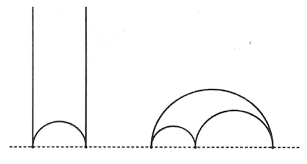
\includegraphics[width=.5\textwidth]{figures/hyperbolic_geometry.png}};
	\end{tikzpicture}
\end{figure}

We define a function $\phi : \mathbb H^2 \to \R / 2\pi\Z$ which to each pair $(p,q)$ of points in the Poincarè half-plane associates the angle between the vector $\vec{q\conj p}$ and the vector $\vec{q p}$ (in this order) or, equivalently, to the angle between the vertical line at $p$ and the geodesic between $p$ and $q$ (in this order):

\begin{figure}[H]
	\centering
	\begin{tikzpicture}
		\node (image) at (0,0) {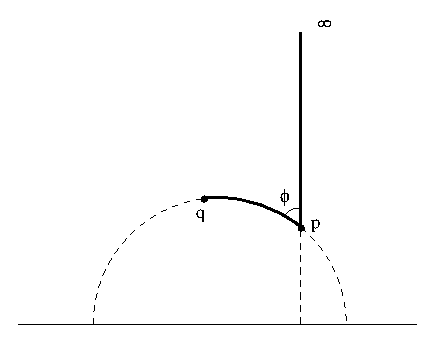
\includegraphics[width=.5\textwidth]{figures/kontsevich_graph_weight.eps}};
	\end{tikzpicture}
\end{figure}

Analytically, $\phi$ is given by
\begin{eqalign}
	(p,q) \longmapsto \arg\left( \frac{q-p}{q-\conj p} \right) = \frac{1}{2i} \log \left( \frac{q-p}{q \conj p} \cdot \frac{\conj q - p}{\conj q - \conj p} \right).
\end{eqalign}
This function is holomorphic over $\mathbb H^2$ and extends continuously to $\Im{p} = 0$ or $\Im{q} = 0$.

Now let $\Gamma \in G_n$ be an admissible graph. Let us denote with $R_n$ the set of possible isometrical embeddings of $\Gamma$ in $\mathbb H$ sending $L$ to $0$ and $R$ to $1$, i.e. the set of possible $n$-tuple of \underline{distinct} points from which we realize geometrically the graph $\Gamma$ using arcs of geodesics to draw the edges. Notice the set $R_n$ is actually independent of $\Gamma$, as any $n$-tuple of distinct points can be used to draw isometrically any graph in $G_n$.

\begin{figure}[H]
	\centering
	\begin{tikzpicture}
		\node (image) at (0,0) {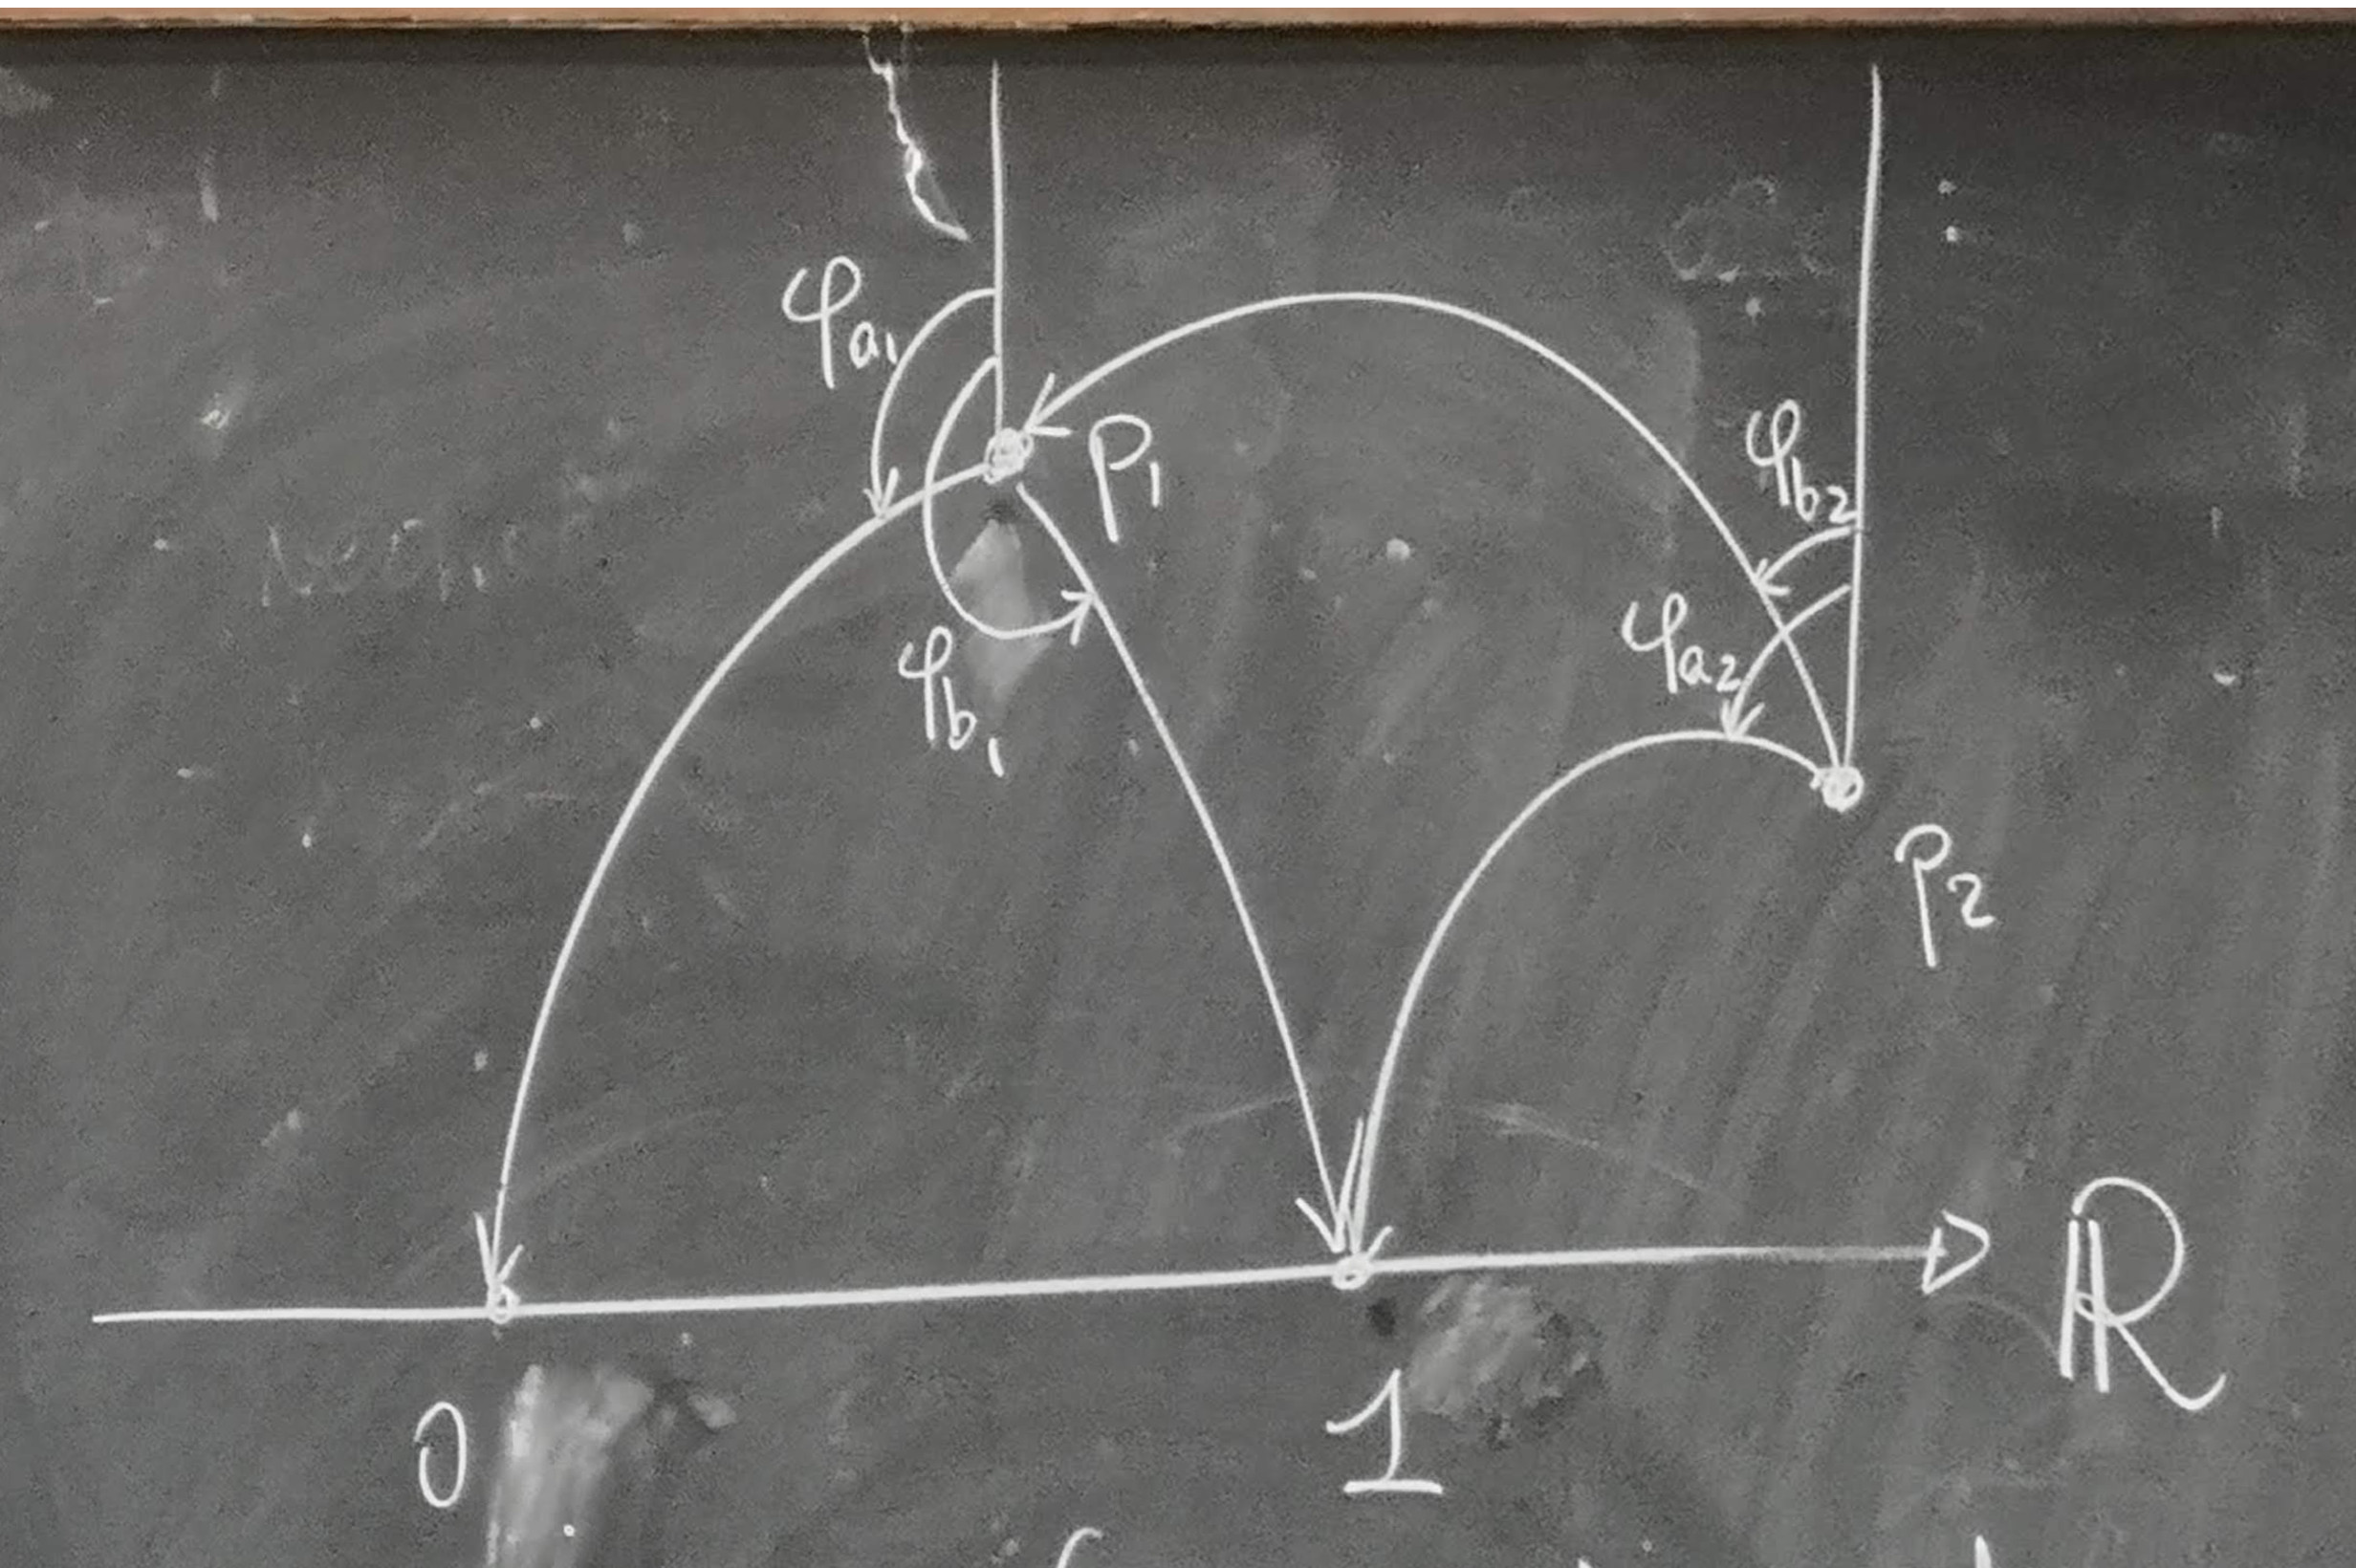
\includegraphics[width=.65\textwidth]{figures/may23_hyperbolic_immersion.jpg}};
	\end{tikzpicture}
	\caption{A realization of the admissible graph \eqref{diag:order_two_adm_graph}.}
	\label{fig:realization_ex}
\end{figure}

Given a realization $V_\Gamma \ni m \mapsto \overline{m} \in \mathbb H$, define $\phi_a$ to be $\phi(\overline{s(a)}, \overline{t(a)})$. Thus $\phi_a$ measure the abovementioned angle for the edge $a$. These are represented in Figure~\ref{fig:realization_ex}.

\begin{definition}
	The weight $w_\Gamma$ associated to $\Gamma \in G_n$ is defined as
	\begin{eqalign}
		w_\Gamma := \frac1{(2\pi)^{2n}} \int_{R_n} \bigwedge_{a \in E_\Gamma} d\phi_a.
	\end{eqalign}
\end{definition}

Then the integral can be done, with a change of variables, in the $\phi_{a_i}, \phi_{b_i}$ coordinates and it can be proven that

\begin{lemma}
	The integral defining $w_\Gamma$ converges absolutely for every admissible graph $\Gamma$.
\end{lemma}

\subsubsection{The formula}
Finally, we can write down the sought formula.

\begin{theorem}
	To a formal Poisson structure $\Pi_\planck$ it is associated the $\star$-product given by
	\begin{eqalign}
		f \star_\planck g := \sum_{n=0}^\infty \frac{\planck^n}{n!} \sum_{\Gamma \in G_n} w_\Gamma B_{\Gamma,\Pi_\planck}(f,g).
	\end{eqalign}
	Moreover, this definition is stable (up to equivalence of $\star$-products) under change of coordinates.
\end{theorem}

\begin{example}
	Let $\Pi_\planck = \Pi = \Pi^{ij} \partial_i \partial_j$, with $\partial_k \Pi^{ij} = 0$ for any $k$. This means that only those $\Gamma \in G_N$ with $t(E_\Gamma) \subseteq \{L,R\}$ contribute to the associated star product, as this guarantees no derivatives of the Poisson tensors appear in their term. Such graphs look like this:
	\begin{diagram}
	\label{diag:moyal_graphs}
		\& \Overset{1}\bullet \arrow{dl} \arrow{drrrr} \& \Overset{2}\bullet \arrow{dll} \arrow{drrr} \&[2ex] \dots \&[2ex] \Overset{n}\bullet \arrow{dllll} \arrow{dr}\\
		\Underset{L}\bullet \& \& \& \& \& \Underset{R}\bullet
	\end{diagram}
	where we didn't label the arrows as for each vertex there are two choices, so for each $n$ we get, in total, $2^n$ non-vanishing terms for the $n$th degree coefficient. The symmetry of exchanging $a_k$ with $b_k$ changes sign to $d\phi_{a_1} \wedge d \phi_{b_1} \wedge \ldots \wedge d\phi_{a_n} \wedge d\phi_{b_n}$, and so does $w_\Gamma$. On the other hand, the corresponding term also changes sign under this exchange, since a term $\Pi^{i_kj_k}$ changes to $\Pi^{j_ki_k} = - \Pi^{i_kj_k}$, by skew-symmetry. In the end, this gets us
	\begin{eqalign}
		B_n(f,g) = \frac1{n!} \sum_{\Gamma \in G_n} w_\Gamma B_{\Gamma, \Pi} = 2^n w_{\Gamma_n} B_{\Gamma_n,\Pi}
	\end{eqalign}
	where $\Gamma_n$ is the graph \eqref{diag:moyal_graphs} labelled as to have all $a_k$ edges going into $L$ and all the $b_k$ into $R$.

	We know what $B_{\Gamma_n, \Pi}$ looks like:
	\begin{eqalign}
		B_{\Gamma_n, \Pi} = \Pi^{i_1j_1} \cdot \ldots \cdot \Pi^{i_nj_n}\, \partial_{i_1}\ldots \partial_{i_n} f \, \partial_{j_1}\ldots \partial_{j_n} g.
	\end{eqalign}
	To compute the weight, we solve the relevant integral. Notice each vertex can be positioned in the same points (i.e. the condition $\overline{1} \neq \overline{2}$ is virtual), and that all angle variables relative to different vertices are independent as there are no edges between them. With these considerations, we can already simplify the computation to the following:
	\begin{eqalign}
		w_\Gamma = \frac1{(2\pi)^{2n}} \int_\hilbert d\phi_{a_1} \wedge d\phi_{b_1} \wedge \ldots \wedge d\phi_{a_n} \wedge d\phi_{b_b} = \frac1{(2\pi)^{2n}} \left( \int_\hilbert d\phi_{a_1} \wedge d\phi_{b_1} \right)^n.
	\end{eqalign}
	Then by fiddling around in the Poincarè upper half-plane, we see that (1) $\phi_a \leq \phi_b$ for any position and (2) all angles are achievable by a suitable configuration of the vertices. Therefore:
	\begin{eqalign}
	\frac1{(2\pi)^{2n}} \left( \int_\hilbert d\phi_{a_1} \wedge d\phi_{b_1} \right)^n = \left( \int_0^{2\pi} \int_0^{\phi_b} d\phi_a d\phi_b \right)^n = \frac1{(2\pi)^{2n}} \left(\frac{2\pi \times 2 \pi}2\right)^n = \frac1{2^n}.
	\end{eqalign}
	So, in the end we get the Moyal product:
	\begin{eqalign}
		f \star g = \frac1{n!} \Pi^{i_1j_1} \cdot \ldots \cdot \Pi^{i_nj_n}\, \partial_{i_1}\ldots \partial_{i_n} f \, \partial_{j_1}\ldots \partial_{j_n} g = f\, \exp\left( \Pi^{ij} \lpartial_i \rpartial_j \right)\, g = f \star_M g.
	\end{eqalign}
\end{example}

\begin{remark}
	The Moyal product is the $\star$-product associated to $\Pi = \Pi^{ij} \partial_i \wedge \partial_j$, where $\Pi^{ij}$ are constants. It's associated to the null deformation. Locally every constant rank Poisson tensor is expressible like that, in Darboux--Weinstein coordinates. This means that, locally, the first-order expansion of the associated product is:
	\begin{eqalign}
		f \star g = fg + \planck\, \Pi^{ij} \partial_i f\, \partial_j g + O(\planck^2).
	\end{eqalign}
\end{remark}

\section{Retrospect}
Our goal was to produce $(\Cinfty(M), \star)$ so as to have observables $f$ in there which obey the equation
\begin{eqalign}
	\partial_t f = \frac{i}\planck [f,h]_\star.
\end{eqalign}
In the undeformed setting, the evolution of $f$ was given by the time evolution operator (ref):
\begin{eqalign}
	f(t) = U(t)^\dagger \,f(0)\, U(t)
\end{eqalign}
In the deformed case we need to correct the operator, starting from the exponential:
\begin{eqalign}
	\exp_\star (g) = 1+g + \frac{g \star g}2 + \frac{g \star g \star g}6 + \ldots = \sum_{n=0}^\infty \frac{g^{\star n}}{n!}.
\end{eqalign}
To get predictions out of the theory, we need necessarily some states on which evaluate observables. Where do we get them? It turns out we can interpret some functions of the algebra as states (the so-called Wigner functions).

\end{document}

	\nocite{*}
	\printbibliography[heading=bibintoc]
\end{document}
